% High-dimensional Gaussian approximation over rectangles.
% Manuscript dated 31 October 2026.
\documentclass[11pt,letterpaper]{article}
\usepackage[margin=1.05in]{geometry}
\usepackage[T1]{fontenc}
\usepackage{lmodern,microtype}
\usepackage{amsmath,amssymb,amsthm,mathtools}
\usepackage{longtable}
\usepackage{tikz}
\usetikzlibrary{arrows.meta}
\usepackage[hidelinks,hypertexnames=false,linktoc=all]{hyperref}
\newcommand{\Ac}{\mathsf A}
\usepackage{fancyhdr}
\pagestyle{fancy}
\fancyhf{}
\fancyhead[L]{\small Gaussian approximation over rectangles}
\fancyhead[R]{\small\thepage}
\setlength{\headheight}{14pt}
\hypersetup{pdftitle={High-Dimensional Gaussian Approximations over Rectangles without Covariance Restrictions},pdfsubject={Bounded independent summands; rates optimal up to logarithmic factors},pdfauthor={Victor Chernozhukov, Denis Chetverikov, Kengo Kato, Yuta Koike}}
\setlength{\parindent}{1.25em}
\setlength{\parskip}{0pt}
\emergencystretch=2em
\allowdisplaybreaks[2]
\raggedbottom
\clubpenalty=10000
\widowpenalty=10000
\newtheorem{theorem}{Theorem}
\newtheorem{proposition}{Proposition}
\newtheorem{lemma}{Lemma}
\newtheorem{corollary}{Corollary}
\newtheorem{conjecture}{Conjecture}
\theoremstyle{remark}
\newtheorem{remark}{Remark}
\newcommand{\E}{\mathbb E}
\newcommand{\Pp}{\mathbb P}
\newcommand{\R}{\mathbb R}
\newcommand{\cR}{\mathcal R}
\newcommand{\cF}{\mathcal F}
\newcommand{\cP}{\mathcal P}
\newcommand{\cD}{\mathcal D}
\newcommand{\Cov}{\operatorname{Cov}}
\newcommand{\Var}{\operatorname{Var}}
\newcommand{\tr}{\operatorname{tr}}
\newcommand{\op}{\mathrm{op}}
\newcommand{\norm}[1]{\left\lVert#1\right\rVert}
\newcommand{\rh}{\rho_{\mathcal R}}
\newcommand{\ind}{\mathbf 1}
\newcommand{\dd}{\,d}
\newcommand{\Hh}{H_2}
\newcommand{\surf}{\mathcal J}

\newcommand{\logp}{\log_+}

\begin{document}
\begin{center}
{\Large High-Dimensional Gaussian Approximations\\[0.15em]
over Rectangles without Covariance Restrictions}\\[0.85em]
{\normalsize Victor Chernozhukov, Denis Chetverikov, Kengo Kato, Yuta
Koike\renewcommand{\thefootnote}{\fnsymbol{footnote}}\footnote{The paper
was developed through collaboration with the AI systems GPT-6 Astra,
GPT-6 Sol, and Claude Opus.}}\\[0.65em]
{\normalsize 31 October 2026}
\end{center}
\setcounter{footnote}{0}
\thispagestyle{plain}

\begin{abstract}
 This paper studies the Gaussian approximation of sums of independent bounded random
vectors over rectangles, with no assumption on the correlation matrix,
which may be singular. Let \(X_1,\ldots,X_n\) be independent centered
random vectors in \(\R^p\) whose coordinates \(X_{ij}\) are bounded in
absolute value by a constant~\(B\), and suppose that each coordinate of
\(W_n\coloneqq n^{-1/2}(X_1+\cdots+X_n)\) has unit variance. Let \(Z_n\) be a
centered Gaussian vector with the covariance matrix of \(W_n\), and put
\(L\coloneqq \log(ep)\) and \(\log_+x\coloneqq \max\{0,\log x\}\). The largest absolute difference
between \(\Pp(W_n\in A)\) and \(\Pp(Z_n\in A)\) over rectangles \(A\) is
at most
\[
 \frac{BL^{3/2}}{\sqrt n}\sqrt{1+\log_+\sqrt{n/L}},
\]
up to a numerical constant. For fixed \(B\) and \(p\asymp n^a\), with
fixed \(a>0\), this bound has order \(n^{-1/2}(\log n)^2\).
If, for a fixed \(c_0>0\), no two distinct coordinates have correlation
larger than \(1-c_0\) in absolute value, the order improves to
\(n^{-1/2}(\log n)^{3/2}\). A further refinement holds if the
third moments cancel in aggregate, that is, if
\(\sum_i\E[X_{ij}X_{ik}X_{i\ell}]=0\) for all coordinates \(j,k,\ell\).
The factor \(BL^{3/2}/\sqrt n\) cannot be improved in general, so the
fixed-gap rate is optimal in this dimension regime, and the unrestricted
rate is optimal up to the factor \((\log n)^{1/2}\). Coordinatewise
truncation extends the bounds to sub-exponential observations, with
additional logarithmic factors.

\end{abstract}

\clearpage
\begingroup
\small
\linespread{0.96}\selectfont
\tableofcontents
\endgroup
\clearpage

\section{\texorpdfstring{Introduction and main results}{Introduction and main results}}\label{sec:results}
Gaussian approximation over rectangles provides a common foundation for
approximating maxima and constructing simultaneous confidence regions, with
applications to a wide variety of statistical inference problems reviewed in~\cite{CCKK2023}.
In many of these applications the correlation matrix may be nearly or
exactly singular. We obtain approximation bounds that remain uniform
as its eigenvalues approach zero.

Let \(W\) be a sum of independent centered bounded random vectors in
\(\R^p\). Suppose that each coordinate of the sum has unit variance,
and let \(Z\) be a centered Gaussian vector with the same covariance.
Our standing assumptions and notation are
\begin{equation}
 \begin{gathered}
 W\coloneqq (W_j)_{j=1}^p=\sum_{i=1}^n\xi_i,\qquad
 \E\xi_i=0,\qquad \norm{\xi_i}_\infty\le\delta\quad\text{a.s.},\\
 \Sigma\coloneqq \Cov(W),\qquad\Sigma_{jj}=1\ (j\le p),
 \qquad Z\sim N(0,\Sigma).
 \end{gathered}
 \label{eq:setup}
\end{equation}
The summands need not have the same distribution, and coordinates within
a summand may be dependent. The unit marginal variances fix the scale
of each coordinate, and they can be obtained by coordinatewise rescaling
whenever all marginal variances are positive. There is no
restriction on the rank of \(\Sigma\).

The parameter \(\delta\) bounds the contribution of any one summand
to any coordinate of \(W\), and such a uniform bound is called an
\emph{envelope}. To state the
bound compactly, put
\[
 L\coloneqq \log(ep),\qquad
 D_L\coloneqq 1+\log_+\frac1{\delta\sqrt L},\qquad
 \log_+x\coloneqq \max\{0,\log x\}.
\]
Here \(L\) encodes the dependence on dimension, while \(D_L\)
contributes an additional logarithmic factor. Constants denoted by
\(C\) are absolute unless a subscript records their dependence.

Let \(\mathcal R\) denote the class of axis-aligned rectangles in
\(\R^p\). We measure the approximation error by the \emph{Kolmogorov distance over rectangles}
\[
 \rh(W,Z)\coloneqq \sup_{A\in\mathcal R}
       |\Pp(W\in A)-\Pp(Z\in A)|.
\]
The same notation is used for any two random vectors in \(\R^p\). For
example, taking \(A\coloneqq (-\infty,s]^p\) shows that this distance controls the
error in approximating the distribution of \(\max_{j\le p}W_j\), the maximum
coordinate of \(W\).

The first bound of this paper depends only on the summand envelope and the
dimension, so it holds uniformly as covariance eigenvalues approach or
reach zero.

\begin{theorem}[Unrestricted covariance]\label{thm:unrestricted}
Under~\eqref{eq:setup},
\begin{equation}
 \rh(W,Z)\le C\min\{1,\delta L^{3/2}\sqrt{D_L}\}.
 \label{eq:unrestricted}
\end{equation}
\end{theorem}

For normalized observations, Theorem~\ref{thm:unrestricted} gives
the following dependence on the sample size.

\begin{corollary}[Normalized observations]\label{cor:observations}
Let \(X_1,\ldots,X_n\in\R^p\) be independent and centered. Suppose
\(\norm{X_i}_\infty\le B\) almost surely and
\(n^{-1}\sum_i\E X_{ij}^2=1\) for every \(j\). Then, with
\(W_n\coloneqq n^{-1/2}\sum_iX_i\) and \(Z_n\sim N(0,\Cov(W_n))\),
\begin{equation}
 \rh(W_n,Z_n)\le C\min\!\left\{1,
 \frac{B L^{3/2}}{\sqrt n}
 \sqrt{1+\log_+\frac{\sqrt n}{B\sqrt L}}\right\}.
 \label{eq:observations-unrestricted}
\end{equation}
\end{corollary}

Corollary~\ref{cor:observations} follows from Theorem~\ref{thm:unrestricted}
by setting \(\xi_i\coloneqq X_i/\sqrt n\), which has envelope \(\delta=B/\sqrt n\). For
fixed \(B\) and \(p\asymp n^a\), with fixed \(a>0\), its bound has
order \(n^{-1/2}(\log n)^2\).

The factor \(BL^{3/2}/\sqrt n\) is sharp. For \(B\ge2\), \(p\to\infty\) and
\(BL^{3/2}/\sqrt n\to0\), Theorem~\ref{opt:skew-lower} gives i.i.d.\ observations
with independent coordinates whose error is at least of order
\(BL^{3/2}/\sqrt n\). The example is inspired by that of Chernozhukov,
Chetverikov, and Koike~\cite[Proposition~2.1]{CCK}, and it drops some of their
side conditions on \(B\) and \(p\). Thus, in this regime, the
bound~\eqref{eq:observations-unrestricted} is optimal up to the logarithmic
factor \(\sqrt{1+\log_+(\sqrt n/(B\sqrt L))}\). When \(p\) grows polynomially
in~\(n\) and \(B\) is fixed, this factor is of order \((\log n)^{1/2}\).
Conjecture~\ref{conj:sharp-unrestricted} states that this factor can be removed.

For unequal marginal variances, let
\[
 \sigma_j^2\coloneqq n^{-1}\sum_i\E X_{ij}^2,
 \qquad
 \underline\sigma\coloneqq \min_j\sigma_j>0.
\]
We then apply Theorem~\ref{thm:unrestricted} to the summands
\(\xi_{ij}\coloneqq X_{ij}/(\sigma_j\sqrt n)\). If
\(\max_i\norm{X_i}_\infty\le K_n\), these summands have
envelope \(\delta=K_n/(\underline\sigma\sqrt n)\).
Positive diagonal scaling maps rectangles to rectangles and so preserves
the distance \(\rh\), and the resulting bound also holds in the
original coordinates.

\subsection{Correlation gaps and third-moment cancellation}
The bound improves when distinct coordinates are separated in
correlation. We measure this separation by the \emph{correlation gap}
\[
 c\coloneqq 1-\max_{j\ne k}|\Sigma_{jk}|,
 \qquad c\coloneqq 1\ \text{when }p=1,
\]
and put
\begin{equation}
 \kappa\coloneqq \begin{cases}\min\{L,c^{-1}\},&c>0,\\L,&c=0,\end{cases}
 \qquad E_\kappa\coloneqq 1+\log_+\frac{\sqrt\kappa}{\delta L}.
 \label{eq:parameters}
\end{equation}
A positive gap excludes equal or opposite coordinates, but permits
singular covariance matrices. The parameter \(\kappa\) selects the
smaller of two smoothing-error bounds: one holds for every covariance
matrix, and the other uses the correlation gap. The factor
\(E_\kappa\) arises when we choose the smoothing width.

\begin{theorem}[Gap-sensitive bound]\label{thm:optimized}
Under~\eqref{eq:setup},
\begin{equation}
 \rh(W,Z)\le C\min\!\left\{1,
 \delta[L^{3/2}+L\sqrt{\kappa E_\kappa}]\right\}.
 \tag{R*}\label{eq:optimized}
\end{equation}
\end{theorem}

Since \(\kappa\le L\) and \(E_\kappa\le D_L\),
Theorem~\ref{thm:optimized} implies Theorem~\ref{thm:unrestricted}.
The term \(\delta L^{3/2}\) in~\eqref{eq:optimized} comes from the
third moments of the summands,
and it disappears when the full \emph{third-moment tensor} cancels.

\begin{theorem}[Cancellation of third moments]\label{thm:zero-skew}
Under~\eqref{eq:setup}, suppose
\begin{equation}
 \sum_i\E\xi_i^{\otimes3}=0,
 \quad\text{equivalently,}\quad
 \sum_i\E[\xi_{ij}\xi_{ik}\xi_{i\ell}]=0
 \quad(j,k,\ell\le p).
 \label{eq:zero-third}
\end{equation}
Then
\begin{equation}
 \rh(W,Z)\le C\min\{1,\delta L\sqrt{\kappa E_\kappa}\}.
 \tag{ZS}\label{eq:zero-skew}
\end{equation}
\end{theorem}

The zero-skewness condition~\eqref{eq:zero-third} holds when each summand is \emph{centrally
symmetric}, that is, when \(\xi_i\) and \(-\xi_i\) have the same law. Because it
involves the mixed third moments \(\E[\xi_{ij}\xi_{ik}\xi_{i\ell}]\), vanishing
marginal third moments do not suffice for this cancellation.

For the normalized observations of Corollary~\ref{cor:observations},
fix \(B\) and suppose \(c\ge c_0>0\). Substituting
\(\delta=B/\sqrt n\) into the preceding two theorems gives
\begin{align}
 \rh(W_n,Z_n)&\le C_{B,c_0}\min\!\left\{1,
 \frac{L^{3/2}}{\sqrt n}
 +\frac L{\sqrt n}\sqrt{1+\log_+\frac{\sqrt n}{L}}\right\},
 \label{eq:observations-fixed}\\
 \rh(W_n,Z_n)&\le C_{B,c_0}\min\!\left\{1,
 \frac L{\sqrt n}\sqrt{1+\log_+\frac{\sqrt n}{L}}\right\}
 \quad\text{under~\eqref{eq:zero-third}}.
 \label{eq:zero-fixed}
\end{align}
In polynomial dimension the bound~\eqref{eq:observations-fixed}
has order \(n^{-1/2}(\log n)^{3/2}\), and it is optimal there, since the
lower-bound examples of~\cite[Proposition~2.1]{CCK} and
Theorem~\ref{opt:skew-lower} have independent coordinates and hence
correlation gap \(1\). These bounds give uniform convergence at a fixed
positive gap when \(\log p=o(n^{1/3})\) in general and \(\log p=o(\sqrt n)\)
under cancellation. Theorem~\ref{opt:consistency} shows that these
conditions are sharp over fixed-envelope classes, with envelope at least
two for the first assertion and at least \(1\) for the second. In
the second case the sharpness concerns only the dimension threshold, and
below the threshold the error rate in~\eqref{eq:zero-fixed} is not known
to be sharp.

\subsection{Polyhedral sets}\label{sec:polyhedra}
A \emph{polyhedron} is an intersection of halfspaces, so membership can be
tested by collecting the scalar products with its face normals into
a vector. The resulting event is a rectangle event in this new space.
To apply the rectangle bounds, we divide each scalar product by its
standard deviation. The condition below ensures that this normalization
leaves the transformed summands uniformly bounded without requiring
the covariance matrix to be invertible.

\begin{corollary}[Gaussian approximation over polyhedra]\label{cor:polyhedra}
Let \(W\coloneqq\sum_{i=1}^n\xi_i\), where the vectors
\(\xi_i\in\R^p\) are independent and centered, with
\(\norm{\xi_i}_\infty\le\delta\) almost surely, for \(\delta>0\).
Set \(\Sigma\coloneqq\Cov(W)\) and let \(Z\sim N(0,\Sigma)\).
For an integer \(m\ge1\) and a constant \(K>0\), let
\(\mathcal P_m(K;\Sigma)\) be the class of polyhedra admitting a
representation
\[
 P=\bigcap_{\alpha=1}^q
 \{x\in\R^p:\nu_\alpha^\top x\le a_\alpha\},
 \qquad 1\le q\le m,
\]
whose normals satisfy
\[
 \sigma_\alpha\coloneqq
 \sqrt{\nu_\alpha^\top\Sigma\nu_\alpha}>0,
 \qquad \norm{\nu_\alpha}_1\le K\sigma_\alpha
 \quad(\alpha=1,\ldots,q).
\]
Put \(\Delta\coloneqq K\delta\) and \(L_m\coloneqq\log(em)\).
Then
\[
 \sup_{P\in\mathcal P_m(K;\Sigma)}
 |\Pp(W\in P)-\Pp(Z\in P)|
 \le C\min\!\left\{1,\,
 \Delta L_m^{3/2}
 \sqrt{1+\log_+\frac1{\Delta\sqrt{L_m}}}\right\},
\]
where \(C\) is an absolute constant. We include the empty set and
\(\R^p\) in the class. No restriction is imposed on the
rank of \(\Sigma\).
\end{corollary}

This transfer uses the reduction to face projections employed by
Chernozhukov, Chetverikov, and Kato~\cite[Section~3.1 and the proof of
Proposition~3.1]{CCK2017} in their extension from rectangles to simple
convex sets. Subsection~\ref{app:polyhedral-transfer} gives the proof
by applying Theorem~\ref{thm:unrestricted} to the standardized
projections.

The condition on the normals is unchanged if a defining inequality
is multiplied by a positive constant. Its role is to bound the size
of each standardized summand:
\[
 \left|\frac{\nu_\alpha^\top\xi_i}{\sigma_\alpha}\right|
 \le\frac{\norm{\nu_\alpha}_1\delta}{\sigma_\alpha}
 \le K\delta=\Delta.
\]
In particular, a uniform bound \(\norm{\nu_\alpha}_1\le B\),
together with \(\sigma_\alpha\ge s_0>0\), gives \(K=B/s_0\).
Thus the number of inequalities enters the bound through \(L_m\),
while the size of the standardized summands enters through \(\Delta\).
Zero-variance directions impose deterministic conditions and are
handled separately in Subsection~\ref{app:polyhedral-transfer}.

Theorems~\ref{thm:optimized} and~\ref{thm:zero-skew} also apply to
these standardized projections. For a representation with \(q\)
inequalities, their correlation matrix is
\[
 R_{\alpha\beta}\coloneqq
 \frac{\nu_\alpha^\top\Sigma\nu_\beta}
      {\sigma_\alpha\sigma_\beta}.
\]
The refinements use dimension \(q\), envelope \(\Delta\), and the
correlation gap of \(R\), which can differ from the gap of the
original coordinates. Aggregate third-moment cancellation is
preserved by the linear transformation. The same appendix subsection
verifies these assertions.

\subsection{Sub-exponential transfer}\label{sec:subexponential}
Truncation provides a second transfer: it extends the bounded theorems
to observations with sub-exponential tails. We first state the rectangle
bounds, then transfer them to polyhedra by the standardized face
projections of Subsection~\ref{sec:polyhedra}. The tail condition is
measured by the \emph{Orlicz norm}
\[
 \|V\|_{\psi_1}\coloneqq \inf\{s>0:\E e^{|V|/s}\le2\}.
\]
If the norm is finite, \(V\) is said to be \emph{sub-exponential}.

\begin{corollary}[Sub-exponential transfer]\label{cor:subexponential}
Let \(X_1,\ldots,X_n\in\R^p\) be independent and centered, with
\(n^{-1}\sum_i\E X_{ij}^2=1\) and
\(\max_{i,j}\|X_{ij}\|_{\psi_1}\le K\), where \(K\ge1\).
For \(W_n\coloneqq n^{-1/2}\sum_iX_i\) and a centered Gaussian \(Z_n\)
with the same covariance, put
\[
 \ell_n\coloneqq \log(en),\qquad b_n\coloneqq \frac{K\ell_n}{\sqrt n},\qquad
 D_n\coloneqq 1+\log_+\frac1{b_n\sqrt L}.
\]
Then
\begin{equation}
 \rh(W_n,Z_n)\le C\min\{1,b_nL^{3/2}\sqrt{D_n}\}.
 \label{eq:subexponential}
\end{equation}
If the correlation gap of \(W_n\) is at least a fixed \(c_0>0\), then
\begin{equation}
 \rh(W_n,Z_n)\le C_{c_0}\min\!\left\{1,
 b_n\left[L^{3/2}+L\sqrt{1+\log_+\frac1{b_nL}}\right]\right\}.
 \label{eq:subexponential-gap}
\end{equation}

For polyhedra, set \(\Sigma\coloneqq\Cov(W_n)\), fix \(J>0\), and
let \(\mathcal P\coloneqq\mathcal P_m(J;\Sigma)\) be the class in
Corollary~\ref{cor:polyhedra}, with at most \(m\) defining inequalities
and \(\norm{\nu_\alpha}_1\le J\sigma_\alpha\), where
\(\sigma_\alpha^2=\nu_\alpha^\top\Sigma\nu_\alpha>0\). Define
\[
 \rho_{\mathcal P}(W_n,Z_n)\coloneqq
 \sup_{P\in\mathcal P}|\Pp(W_n\in P)-\Pp(Z_n\in P)|,
 \qquad K_{\mathcal P}\coloneqq\max\{1,JK\}.
\]
Then~\eqref{eq:subexponential} also holds with
\(\rh\), \(K\), and \(L\) replaced throughout by
\(\rho_{\mathcal P}\), \(K_{\mathcal P}\), and
\(L_m=\log(em)\), respectively. The same replacement
in~\eqref{eq:subexponential-gap} holds for any subclass whose members
admit representations with
\[
 \left|\frac{\nu_\alpha^\top\Sigma\nu_\beta}
 {\sigma_\alpha\sigma_\beta}\right|\le1-c_0
 \qquad(\alpha\ne\beta).
\]
Here the gap condition is imposed on the standardized face projections.
\end{corollary}

The bound~\eqref{eq:subexponential} requires neither a lower bound on a
local determinant nor a lower bound on the positive eigenvalues of the
covariance matrix of \(W_n\). For unequal marginal variances, the tail
condition is imposed on \(X_{ij}/\sigma_j\), as in the standardization after
Corollary~\ref{cor:observations}. The polyhedral transfer follows from
\[
 \left\|\frac{\nu_\alpha^\top X_i}{\sigma_\alpha}\right\|_{\psi_1}
 \le \frac{K\norm{\nu_\alpha}_1}{\sigma_\alpha}
 \le JK\le K_{\mathcal P}.
\]
Thus the same tail argument applies after projection, with the number
of defining inequalities replacing the ambient dimension. A correlation
gap in the original coordinates does not by itself ensure a gap among
these projections.

For fixed \(K\) and \(p\asymp n^a\) with \(a>0\) fixed, the
bound~\eqref{eq:subexponential} is of order \(n^{-1/2}(\log n)^3\), and the
bound~\eqref{eq:subexponential-gap} under a fixed correlation gap is of order
\(n^{-1/2}(\log n)^{5/2}\), so the power \(n^{-1/2}\) of the sample size is
again optimal up to logarithmic factors. By~\eqref{eq:subexponential}, the error
tends to zero for fixed \(K\) when \(\log p=o(n^{1/3}/\log(en))\).
Appendix~\ref{app:subexponential} proves the rectangle bounds by
clipping each coordinate at a level of order \(K\log(en)\).
Exponential moments control the discarded sum, and a joint Gaussian
coupling restores the original covariance. For polyhedra, the proof
first forms the standardized face projections and applies this same
argument at tail scale \(K_{\mathcal P}\), so no additional truncation
or Gaussian comparison is needed.

\subsection{Relation to recent work}\label{sec:literature}
High-dimensional Gaussian approximation for maxima and rectangles was
developed by Chernozhukov, Chetverikov, and Kato~\cite{CCK2013,CCK2017}.
Without covariance restrictions beyond positive marginal variances,
Chernozhukov, Chetverikov, Kato, and Koike~\cite[Theorem~2.1]{CCKK2022}
obtained an \(n^{-1/4}\) rate, up to logarithms, under coordinatewise
sub-exponential tails and an averaged fourth-moment condition.
The cube-root rectangle bound reported in~\cite[Theorem~1 and Section~5]{GaoZhang} improves the sample-size power to \(n^{-1/3}\). Under the tail assumption of Corollary~\ref{cor:subexponential}, in the unit-variance notation of this paper, it is
\begin{equation*}
 C\min\left\{1,
 \left(\frac{K^2}{n}\right)^{1/3}\{\log(2np)\}^{7/3}
 +\frac K{\sqrt n}\{\log(2np)\}^{5/2}\right\}.
\end{equation*}
No additional fourth-moment condition is needed for this bound.
For fixed \(K\) and \(p\asymp n^a\), with fixed \(a>0\), it has
order \(n^{-1/3}(\log n)^{7/3}\). In this dimension regime,
Corollaries~\ref{cor:observations} and~\ref{cor:subexponential}, with
fixed \(B\) or \(K\), give the sharp sample-size power
\(n^{-1/2}\), with logarithmic factors \((\log n)^2\) for bounded
observations and \((\log n)^3\) for sub-exponential coordinates.
These comparisons concern fixed envelopes or tail scales. The full
bounds retain their different dependence on these parameters.

A second line of work obtains rates close to \(n^{-1/2}\) under
covariance nondegeneracy. For bounded sums with positive definite
\(\Sigma\), the nondegenerate \(n^{-1/2}\) bound reported in~\cite[Theorem~1.1]{AL} removes the
\(\log(en)\) factor from the bound of Chernozhukov, Chetverikov,
and Koike~\cite[Corollary~2.1]{CCK}, and reads
\begin{equation*}
 \rh(W_n,Z_n)\le C\min\left\{1,
 \frac{BL^{3/2}}{\lambda_{\min}(\Sigma)\sqrt n}\right\}.
\end{equation*}
A fixed positive minimum eigenvalue therefore gives the sharp
\(BL^{3/2}/\sqrt n\) scale in the regimes of matching lower
bounds~\cite[Proposition~2.1]{CCK}.
The unrestricted bound of this paper does not involve \(\lambda_{\min}(\Sigma)\),
and it exceeds this scale only by the factor \(\sqrt{D_L}\).

Other results replace full nondegeneracy by conditions on small
groups of coordinates. Fang, Koike, Liu, and Zhao~\cite[Theorem~1.1]{FKLZ} obtain nearly
\(n^{-1/2}\) rates under sub-exponential tails and quantitative
two- and three-coordinate covariance conditions, allowing the full
covariance matrix to be singular. The companion paper~\cite{Local}
assumes uniformly positive eigenvalues for principal submatrices of
order at most four. For bounded observations it gives
\(C_aBL^{3/2}/\sqrt n\), and \(C_aBL/\sqrt n\) under aggregate
third-moment cancellation. The present results also cover singular
three- and four-coordinate submatrices. For general bounded observations,
the unrestricted bound here has an additional factor \(\sqrt{D_L}\).
Under third-moment cancellation, the companion paper's
\(C_aBL/\sqrt n\) rate is sharper than the unrestricted bound obtained
here.

The proof compares the sum with its Gaussian counterpart along
covariance-preserving interpolations. We smooth the rectangle indicator,
then control its derivatives through the aggregate covariance and
concentration near the rectangle boundary. These estimates avoid
inverse covariance eigenvalues and remain valid when the covariance
matrix is singular.

The next subsection records the scope of formal verification in Lean.
Section~\ref{sec:smoothing} then outlines the proof, introduces its
notation, and derives the rates from the main estimates.
Section~\ref{opt:section} discusses sharpness and open questions.
Appendices~\ref{sec:main-proof}--\ref{app:subexponential} prove the
upper bounds, and Appendix~\ref{app:sharpness-proofs} proves the
lower bounds and consistency criteria. All proofs of the results stated
here are included in this paper. The
Supplement~\cite{Supplement} contains additional calculations and
related investigations.

\subsection{\texorpdfstring{Formal verification in Lean}{Formal verification in Lean}}\label{sec:lean-certification}
Lean is a proof assistant that checks formal mathematical proofs by
computer. A separate Lean development establishes
Theorems~\ref{thm:unrestricted}--\ref{opt:consistency} and the two
rectangle bounds of Corollary~\ref{cor:subexponential}. These proofs
were checked on 20 and 21~October 2026 using Lean~4.19.0 and
mathlib~v4.19.0, and use only Lean's standard axioms. The
\href{https://github.com/VC2015/HDCLTs/blob/bbf1ab99c733a398c181ca8c9f5a243a41f258c6/verification/2026-10-21-companion-results/README.md}{verification record}
contains the Lean sources, axiom audits, and statement-correspondence
reviews for source revision
\href{https://github.com/VC2015/HDCLTs/commit/6548201a5c5d9c132a53f1d504f7ef70346aa782}{\texttt{6548201a5c5d}}.

That record certifies the specified results through their Lean proofs.
A formal verification of the complete interpolation argument presented
here, including the general interpolation identity and smooth Gaussian
initialization, remains to be carried out.
Theorems~\ref{opt:symmetric-lower}--\ref{opt:q4-growing} and
the polyhedral extensions in Corollaries~\ref{cor:polyhedra}
and~\ref{cor:subexponential}
are also outside the certification. The record therefore does not
certify every result or written derivation in this paper, or the
Supplement as a whole.

\section{Outline of the proof}
\label{sec:smoothing}

We prove the rectangle bounds by replacing each rectangle indicator
by a smooth approximation, comparing its expectations under the sum
and the Gaussian target, and then choosing the smoothing width.
This comparison between the smoothed expectations under the sum and
the Gaussian target must allow singular covariance matrices and nonzero
third moments, with estimates that do not involve inverse covariance
eigenvalues. We work on the linear subspace supporting the sum and
follow a path that preserves covariance while replacing bounded
summands by Gaussian noise.

We first add a small independent Gaussian component and normalize
the result to preserve covariance. We then gradually delete summands
and rescale those retained while increasing the Gaussian variance.
The initial Gaussian component permits Gaussian integration by parts
throughout the main comparison, and our choice of rescaling controls
the third-moment contribution near the starting point.
Subsection~\ref{sec:outline-smoothing} gives the smoothing bound,
Subsections~\ref{sec:outline-path}--\ref{sec:outline-seeded} explain
the comparison, and Subsection~\ref{sec:rate} derives the rates.
The detailed estimates and their proofs are in
Appendices~\ref{sec:main-proof}--\ref{appx-app:concentration}.


\subsection{Support coordinates and the logistic approximation}
\label{sec:outline-smoothing}

A bounded closed rectangle is specified by one lower and one upper
inequality for each coordinate, giving \(m\coloneqq2p\) inequalities
in all. It suffices to prove uniform bounds for these rectangles,
since the result for general rectangles follows by monotone approximation.

We now make a change of coordinates such that the aggregate covariance
is the identity. Let \(r\coloneqq\operatorname{rank}(\Sigma)\), and
choose a \(p\times r\) matrix \(\Gamma\) with linearly independent
columns such that \(\Sigma=\Gamma\Gamma^\top\). Each summand lies
almost surely in its range: indeed, if \(z\) is in the null space of
\(\Sigma\), independence and centering give
\(\sum_i\E(z^\top\xi_i)^2=z^\top\Sigma z=0\). Now define
\[
 \zeta_i^0\coloneqq(\Gamma^\top\Gamma)^{-1}\Gamma^\top\xi_i,
 \qquad S\coloneqq\sum_i\zeta_i^0,
 \qquad G\sim N(0,I_r),
\]
where \(G\) is independent of the summands. The vectors
\(\zeta_i^0\in\R^r\) remain independent and centered, and
\[
 \xi_i=\Gamma\zeta_i^0,\qquad
 W=\Gamma S,\qquad Z=\Gamma G,\qquad
 \sum_i\E\zeta_i^0(\zeta_i^0)^\top=I_r.
\]
We call \(\zeta_i^0\) the \emph{support coordinates} of \(\xi_i\).
The superscript \(0\) distinguishes these summands from their
independent copies used later. From this point on, we carry out the
smoothing and interpolation arguments in \(\R^r\).

We first write the rectangle as a system of linear inequalities, then
express those inequalities in support coordinates. A vector
\(y\in\R^p\) belongs to \(B=\prod_{j=1}^p[\ell_j,b_j]\) if and
only if \(\ell_j\le y_j\le b_j\) for every \(j\). Let \(e_j\)
denote the \(j\)th standard basis vector, and let \(\cdot\) denote
the usual inner product. Writing both bounds with the inequality
sign \(\le\), we obtain
\[
 y\in B\quad\Longleftrightarrow\quad
 e_j\cdot y\le b_j\ \text{and}\ (-e_j)\cdot y\le-\ell_j,
 \qquad j=1,\ldots,p.
\]

On the covariance support, we write \(y=\Gamma x\), where
\(x\in\R^r\). Since
\(e_j\cdot(\Gamma x)=(\Gamma^\top e_j)\cdot x\), these inequalities
become
\[
 \Gamma x\in B\quad\Longleftrightarrow\quad
 (\Gamma^\top e_j)\cdot x\le b_j\ \text{and}\
 (-\Gamma^\top e_j)\cdot x\le-\ell_j,
 \qquad j=1,\ldots,p.
\]
We therefore define the \emph{face normals} in support coordinates by
\[
 u_j\coloneqq\Gamma^\top e_j,\qquad
 u_{p+j}\coloneqq-\Gamma^\top e_j,
 \qquad j=1,\ldots,p.
\]
There are \(m=2p\) normals, one for each lower or upper inequality.

These vectors are the outward normals of the half-spaces defining
the transformed rectangle. The original coordinates have variance
\(1\), so
\[
 \|u_j\|^2=\|\Gamma^\top e_j\|^2=e_j^\top\Sigma e_j=1.
\]
The opposite normals \(u_{p+j}=-u_j\) also have unit length.
Different coordinate inequalities may give the same normal, so
repeated normals are allowed.

Next, we collect the upper and lower thresholds into one vector
\(a\in\R^m\) by setting
\[
 a_j\coloneqq b_j,\qquad a_{p+j}\coloneqq-\ell_j,
 \qquad j=1,\ldots,p.
\]
The transformed inequalities then describe the set
\[
 A_a\coloneqq\{x\in\R^r:u_\alpha\cdot x\le a_\alpha
                   \text{ for every }\alpha=1,\ldots,m\}.
\]
Thus \(\Gamma x\in B\) if and only if \(x\in A_a\). We allow
arbitrary finite threshold vectors. If the inequalities are
inconsistent, the set is empty, as happens when a lower endpoint
exceeds its upper endpoint.

This correspondence lets us express the original probability
comparison entirely in support coordinates. Since \(W=\Gamma S\)
and \(Z=\Gamma G\), we have
\[
 \Pp(W\in B)=\Pp(S\in A_a),\qquad
 \Pp(Z\in B)=\Pp(G\in A_a).
\]
As \(B\) ranges over bounded closed rectangles, \(a\) ranges over
\(\R^m\). The approximation error is therefore
\[
 \rho\coloneqq\sup_{a\in\R^m}
 |\Pp(S\in A_a)-\Pp(G\in A_a)|=\rh(W,Z).
\]

The original coordinate bound \(|\xi_{ij}|\le\delta\) also bounds
the component of \(\zeta_i^0\) along each face normal. Indeed,
\(\Gamma\zeta_i^0=\xi_i\) gives
\[
 u_j\cdot\zeta_i^0=\xi_{ij},\qquad
 u_{p+j}\cdot\zeta_i^0=-\xi_{ij}.
\]
Thus each such component is an original coordinate, up to sign.

To measure all these components together, define the \emph{face norm}
\[
 \norm x_U\coloneqq\max_{\alpha\le m}|u_\alpha\cdot x|
                  =\norm{\Gamma x}_\infty.
\]
This is a norm because \(\Gamma\) is injective. The original summand
bound now gives
\[
 \norm{\zeta_i^0}_U=\norm{\xi_i}_\infty\le\delta.
\]
In particular, the bound is unaffected by small positive eigenvalues
of \(\Sigma\). This is the coordinate reduction used
in~\cite[Section~2.3]{GaoZhang}.

The assumptions for the refined bounds also have direct interpretations
in these coordinates. Recall that \(c\) is the correlation gap, so
\(|\Sigma_{jk}|\le1-c\) for \(j\ne k\). For the upper-face normals,
\[
 u_j\cdot u_k=e_j^\top\Sigma e_k=\Sigma_{jk}.
\]
Reversing a normal changes the sign of the inner product.
Consequently, normals from different coordinates have inner product
at most \(1-c\), while opposite normals from the same coordinate
have inner product \(-1\). Hence
\[
 u_\alpha\cdot u_\beta\le1-c\qquad\text{whenever }\alpha\ne\beta.
\]

Finally, the coordinate change is linear and invertible on the
covariance support, so it preserves aggregate third-moment
cancellation. The zero-skewness assumption~\eqref{eq:zero-third}
is therefore equivalent to
\begin{equation}
 \sum_i\E(\zeta_i^0)^{\otimes3}=0.
 \label{eq:zero-third-support}
\end{equation}


We now replace the indicator of \(A_a\) by a smooth function so that
we can compare its expectations under \(S\) and \(G\) by interpolation.
Let \(\ind_{A_a}\) denote
the indicator of \(A_a\), equal to \(1\) on the set and zero outside.
For a \emph{smoothing width} \(h>0\), define its
\emph{logistic approximation} by
\begin{equation}
 F_{a,h}(x)\coloneqq
 \left(1+\sum_{\alpha=1}^m
 e^{(u_\alpha\cdot x-a_\alpha)/h}\right)^{-1},
 \qquad x\in\R^r.
 \label{eq:selector}
\end{equation}
We index the approximation by the threshold vector \(a\), which
specifies the formula even when some defining inequalities are redundant.
For each fixed \(x\), this formula induces a probability distribution
over the \(m\) faces and an additional \emph{baseline option}. Face
\(\alpha\) receives weight proportional to \(e^{(u_\alpha\cdot x-a_\alpha)/h}\),
while the baseline option receives weight proportional to \(1\). After normalization,
the baseline probability is \(F_{a,h}(x)\), and the \emph{face probabilities}
sum to \(1-F_{a,h}(x)\). We use these probabilities below to express
and bound the derivatives of the logistic approximation.

We compare the sum \(S\) and the standard Gaussian vector \(G\)
through the expectations of these smooth functions. Their largest
discrepancy is
\begin{equation}
 M_h\coloneqq\sup_{a\in\R^m}
 \left|\E F_{a,h}(S)-\E F_{a,h}(G)\right|.
 \label{eq:smoothed-discrepancy}
\end{equation}
The interpolation argument will bound \(M_h\). Combining this
bound with the error from replacing indicators by their logistic
approximations will then bound \(\rho\).

Membership in \(A_a\) requires the largest face-inequality violation
to be nonpositive. The logistic approximation smooths both the maximum
and the indicator that tests this condition. We can write
\[
 F_{a,h}(x)=g_h\!\left(h\log\sum_{\alpha=1}^m
 e^{(u_\alpha\cdot x-a_\alpha)/h}\right),
 \qquad g_h(s)\coloneqq\frac1{1+e^{s/h}}.
\]
The inner function smoothly approximates the maximum violation, while
\(g_h\) approximates the indicator of \(({-\infty},0]\). We use the
same scale \(h\) for both steps. The construction of Chernozhukov,
Chetverikov, and Kato~\cite{CCK2013} allows the cutoff function and
its scale to be chosen separately from the smooth maximum. The
resulting multinomial logistic form, with a baseline score of zero,
was used by McFadden~\cite[p.~1001]{McFadden1989} to smooth indicators
of simultaneous inequalities and also appears in~\cite[eq.~(5)]{GaoZhang}.
For every \(h>0\), the approximation is smooth, allowing us to
differentiate along the interpolation path. As \(h\) decreases to
zero, it approaches the indicator away from the boundary, but the
uniform bounds on its derivatives increase.

An anti-concentration inequality controls the probability of falling
in the boundary layer created by moving the thresholds. Write
\[
 A_a^s\coloneqq\{x:u_\alpha\cdot x\le a_\alpha+s
                         \text{ for all }\alpha\le m\}.
\]
The next lemma is the rectangle anti-concentration bound expressed
through the \(m=2p\) face inequalities. Recall that \(L=\log(ep)\),
so \(\log(em)\le(1+\log2)L\).
\begin{lemma}[Rectangle anti-concentration]\label{lem:concentration}
Let \(X_1,\ldots,X_n\in\R^r\) be independent centered random
vectors, and put \(V\coloneqq\sum_iX_i\). Suppose that
\[
 \norm{X_i}_U\le\eta\quad\text{almost surely for every }i,
 \qquad \Var(u_\alpha\cdot V)=v>0
                   \quad\text{for every }\alpha\le m.
\]
Let \(R\in\R^r\) be a random vector independent of the summands.
Then, for every \(a\in\R^m\) and \(s>0\),
\[
 \Pp(V+R\in A_a^s\setminus A_a^{-s})
 \le C\min\{1,(s+\eta)\sqrt{L/v}\}.
\]
If instead \(V\) is a centered Gaussian vector with
\(\Var(u_\alpha\cdot V)=v>0\) for every \(\alpha\), the same
bound holds with \(\eta=0\) for every \(R\) independent of \(V\).
The constant \(C\) is absolute.
\end{lemma}
Appendix~\ref{appx-app:concentration} proves the bounded-sum assertion
by conditioning on pairs of independent copies and applying the
Rademacher anti-concentration inequality of O'Donnell, Servedio,
and Tan~\cite{OST}, in the form recorded
in~\cite[Lemma~J.4]{CCKK2022}. This recovers the bounded-sum estimate
in~\cite[Lemma~2.1]{AL}, obtained using a bootstrap argument and
Kane's~\cite{Kane} noise-sensitivity inequality. The Gaussian assertion
is Nazarov's inequality applied to the vector
\((u_\alpha\cdot V)_{\alpha\le m}\), as stated
in~\cite[Lemma~A.1]{CCK2017}.

Recall that \(\kappa=\min\{L,c^{-1}\}\), interpreted as
\(\kappa=L\) when \(c=0\). The following lemma bounds the error
of the logistic approximation and connects the smoothed discrepancy
\(M_h\) to the desired probability bound.
\begin{lemma}[Smoothing error]\label{lem:endpoint}
Under~\eqref{eq:setup}, for \(h\ge\delta\), uniformly in
\(a\in\R^m\),
\begin{equation}
 \E|F_{a,h}(S)-\ind_{A_a}(S)|+
 \E|F_{a,h}(G)-\ind_{A_a}(G)|\le Ch\sqrt L\,\kappa.
 \label{eq:endpoint-error}
\end{equation}
Consequently,
\begin{equation}
 \rho\le M_h+Ch\sqrt L\,\kappa.
 \label{eq:endpoint-min}
\end{equation}
\end{lemma}

To bound the smoothing error without assuming a positive correlation
gap, let \(\omega_0,\omega_1,\ldots,\omega_m\) be independent
exponential random variables with mean \(1\), independent of \(S\) and
\(G\). The logistic approximation has the exact representation
\begin{equation}
 \begin{split}
 F_{a,h}(x)&=\Pp_\omega(x\in A_{a,\omega}),\\
 A_{a,\omega}&\coloneqq\{x:u_\alpha\cdot x\le
 a_\alpha+h\log(\omega_\alpha/\omega_0)
                   \text{ for all }\alpha\le m\}.
 \end{split}
 \label{eq:mixture}
\end{equation}
This is also the classical \emph{random-utility representation}
underlying multinomial logit probabilities, as described
by Yellott~\cite[Section~2.6]{Yellott1977}. Indeed, the variables
\(-\log\omega_\beta\), \(0\le\beta\le m\), are independent
\emph{standard Gumbel variables}, and \(F_{a,h}(x)\) is the probability
that the baseline utility \(-h\log\omega_0\) exceeds all face utilities
\(u_\alpha\cdot x-a_\alpha-h\log\omega_\alpha\).

For the smoothing bound, we use \eqref{eq:mixture} as a representation
by random threshold shifts with the face normals fixed.
The expected largest absolute threshold shift is at most
\(ChL\), so anti-concentration bounds the smoothing error by
\(ChL^{3/2}\). When \(c>0\), separation of the face normals
allows a sharper bound, \(Ch\sqrt L/c\), through the second
derivatives of the logistic potential. Taking the smaller bound
gives the factor \(\kappa\) in Lemma~\ref{lem:endpoint}.
Lemmas~\ref{appx-lem:endpoint-free} and~\ref{appx-lem:endpoint-gap}
prove these two estimates.

The derivatives used in the interpolation are sums of products of
face components, weighted by the face probabilities. Their total
weight is controlled by \(F_{a,h}(1-F_{a,h})\), which is concentrated
near the boundary. Anti-concentration therefore supplies a small
factor when these derivatives are averaged. In particular,
\[
 \E F_{a,h}(U)(1-F_{a,h}(U))\le Ch\sqrt L
\]
whenever \(U\) has the boundary-concentration property specified in
Lemma~\ref{appx-lem:envelope}. We retain the individual face components
until after summing over the observations, so that the covariance
identity can control two of them. Appendix~\ref{appx-sec:mixture}
derives the derivative formulas and their local bounds from the
higher-order chain rule~\cite{Comtet1974}, and the formulas also
appear in~\cite[Lemma~13]{GaoZhang}.

\subsection{Calibrated dropout with Slepian regularization}
\label{sec:outline-path}

We compare the smoothed expectations by gradually deleting the bounded
summands and replacing them with Gaussian noise. For a fixed
\(\varepsilon>0\) and time index \(t\in[0,1]\), consider the path
\begin{equation}
 U_t\coloneqq
 \frac{(1+t)\sum_{i=1}^n\mathbb B_{i,t}\zeta_i^0
             +\sqrt{t+\varepsilon}\,G}{\sqrt{1+\varepsilon}},
 \qquad 0\le t\le1.
 \label{eq:path}
\end{equation}
At each fixed time, the \(\mathbb B_{i,t}\) are independent Bernoulli
\emph{masks}, independent of the summands and \(G\). A mask equal to \(1\) retains
its summand, and a mask equal to zero deletes it. Before the common
normalization, each retained summand is multiplied by its \emph{amplitude}
\(\gamma(t)\coloneqq1+t\). The \emph{retention probability} is
\[
 \varpi(t)\coloneqq\Pp(\mathbb B_{i,t}=1)
             =\frac{1-t}{(1+t)^2}.
\]
These choices give \(\varpi(t)\gamma(t)^2=1-t\). In the normalized
path~\eqref{eq:path}, the two independent components therefore contribute
\[
 \underbrace{\frac{1-t}{1+\varepsilon}I_r}_{\text{retained summands}}
 +\underbrace{\frac{t+\varepsilon}{1+\varepsilon}I_r}_{\text{Gaussian component}}
 =I_r.
\]
As \(t\) increases, covariance is transferred from the retained summands
to the Gaussian component, while \(\Cov(U_t)=I_r\) throughout.
At \(t=0\), every summand is retained. At \(t=1\), all summands have
been deleted, leaving only the Gaussian vector.

This random deletion is known as \emph{Bernoulli thinning}
\cite{Renyi1956,SteutelHarn1979,LastPenrose2017}. We call the
chosen amplitude and retention probability \emph{calibrated dropout},
in reference to the independent masks used in dropout regularization~\cite{Dropout2014}.
With \(\varepsilon=0\), this coincides with the calibrated path
defined in~\cite[Section~4]{AL}. Before normalization, each summand's third-moment tensor is multiplied
by \(\varpi(t)\gamma(t)^3=1-t^2\). The derivative of this multiplier
conveniently vanishes at \(t=0\), which will help control the impact of
the third moments when the Gaussian variance is smallest.

The extra Gaussian variance \(\varepsilon\), called the
\emph{Gaussian seed}, keeps that variance positive from the start.
The endpoints of the interpolation are
\[
 U_0=\frac{S+\sqrt\varepsilon\,G}{\sqrt{1+\varepsilon}},
 \qquad U_1=G.
\]
To reach \(U_0\) from \(S\), we first follow the short
\emph{Slepian interpolation}
\[
 T_v\coloneqq\sqrt{1-v}\,S+\sqrt v\,G,\qquad 0\le v\le1,
\]
from \(v=0\) to \(v_\varepsilon\coloneqq
\varepsilon/(1+\varepsilon)\), so that \(T_{v_\varepsilon}=U_0\).
We call this initial operation \emph{Slepian regularization}.
After a change of time it is also
\emph{Ornstein--Uhlenbeck regularization}~\cite[Theorem~4.12]{Nourdin2012}.

Figure~\ref{fig:two-stage-path} summarizes the two stages. Slepian
regularization rescales every summand and adds a small Gaussian component.
The calibrated dropout path then deletes summands at random, amplifies
those retained, and increases the Gaussian variance. Both stages preserve
covariance \(I_r\). The paths describe distributions at each time, and
we do not need to couple the Bernoulli masks across different times.

\begin{figure}[htbp]
\centering
\resizebox{\textwidth}{!}{%
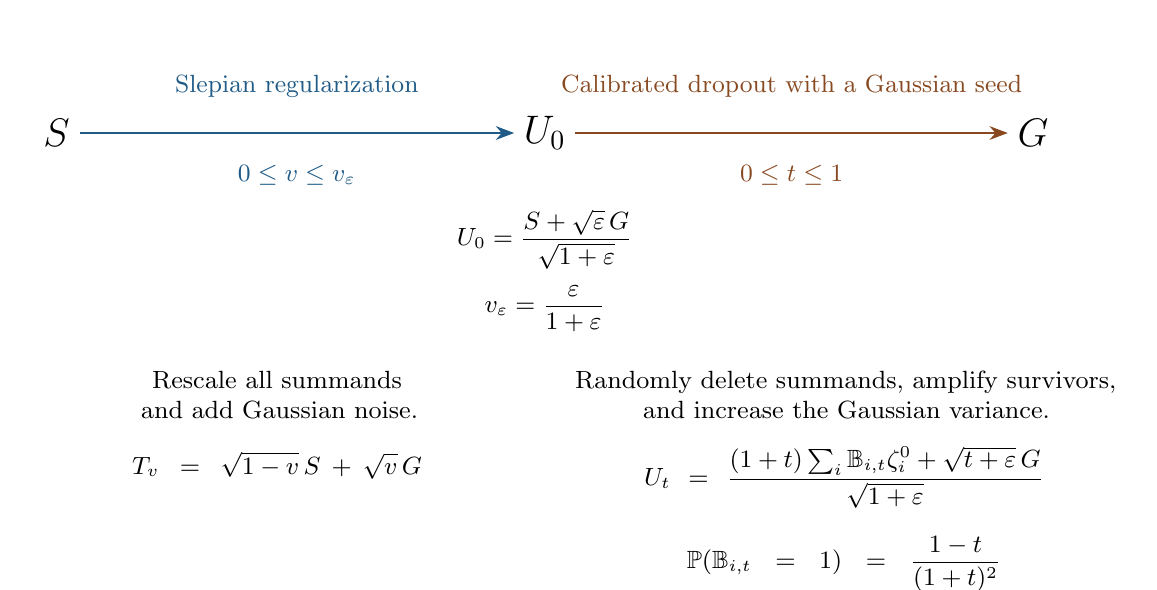
\begin{tikzpicture}[>=Stealth,font=\fontsize{9}{11}\selectfont]
\definecolor{seed}{RGB}{32,91,135}
\definecolor{drop}{RGB}{136,73,32}
\node[font=\Large] (S) at (0,0) {$S$};
\node[font=\Large] (U) at (6.2,0) {$U_0$};
\node[font=\Large] (G) at (12.4,0) {$G$};
\draw[->,thick,seed] (S) -- node[above=9pt,align=center] {Slepian regularization} node[below=8pt] {$0\le v\le v_\varepsilon$} (U);
\draw[->,thick,drop] (U) -- node[above=9pt,align=center] {Calibrated dropout with a Gaussian seed} node[below=8pt] {$0\le t\le1$} (G);
\node[anchor=north,align=center] at (6.2,-0.85) {$\displaystyle U_0=\frac{S+\sqrt\varepsilon\,G}{\sqrt{1+\varepsilon}}$
\\[5pt] $\displaystyle v_\varepsilon=\frac{\varepsilon}{1+\varepsilon}$};
\node[anchor=north,align=center,text width=6.1cm] at (2.8,-2.9) {Rescale all summands and add Gaussian noise.\\[9pt]
 $\displaystyle T_v=\sqrt{1-v}\,S+\sqrt v\,G$};
\node[anchor=north,align=center,text width=7.0cm] at (10,-2.9) {Randomly delete summands, amplify survivors,\\and increase the Gaussian variance.\\[9pt]
 $\displaystyle U_t=\frac{(1+t)\sum_i\mathbb B_{i,t}\zeta_i^0+\sqrt{t+\varepsilon}\,G}{\sqrt{1+\varepsilon}}$\\[9pt]
 $\displaystyle \mathbb P(\mathbb B_{i,t}=1)=\frac{1-t}{(1+t)^2}$};
\end{tikzpicture}
}
\caption{The comparison from \(S\) to \(G\) passes through the regularized
sum \(U_0\). The first stage follows \(T_v\) up to \(v_\varepsilon\),
and the second follows \(U_t\) from \(t=0\) to \(t=1\).}
\label{fig:two-stage-path}
\end{figure}

We first compare \(S\) with \(U_0\), and then \(U_0\) with \(G\).
For fixed thresholds, write
\[
 P_a(t)\coloneqq\E F_{a,h}(U_t),\qquad
 I_h\coloneqq\sup_a|\E F_{a,h}(S)-\E F_{a,h}(U_0)|.
\]
The quantity \(I_h\) measures the error from introducing the seed.
The triangle inequality and the smoothing lemma give
\begin{equation}
 \rho\le M_h+Ch\sqrt L\,\kappa,\qquad
 M_h\le I_h+\sup_a\int_0^1|P_a'(t)|\dd t,
 \label{eq:roadmap}
\end{equation}
where \(P_a'(t)\) is the time derivative of \(P_a(t)\), measuring
the rate of change of the smoothed probability at time \(t\).
The smoothing error is evaluated at the original endpoints \(S\)
and \(G\). It remains to bound the initialization error and the
derivative along the seeded path.

\subsection{Controlling the comparison error}
\label{sec:outline-seeded}

To bound the integral in~\eqref{eq:roadmap}, we need an expression
for how \(P_a(t)\) changes along the interpolation. The identity below
separates a term involving the aggregate third moments from a remainder
involving fourth derivatives. Let
\(K_3\coloneqq\sum_i\E(\zeta_i^0)^{\otimes3}\) be the aggregate
third-moment tensor. Lemma~\ref{appx-an:lem:identity} gives
\begin{equation}
 P_a'(t)=
 -\frac{t}{3(1+\varepsilon)^{3/2}}\,
       \E D^3F_{a,h}(U_t):K_3+R_{4,a,h}(t).
 \label{eq:path-summary}
\end{equation}
Here \(D^3F\) is the third derivative tensor, and the colon sums
products of corresponding tensor entries. The remainder involves
fourth derivatives evaluated at nearby points. Evaluating all third
derivatives at the common point \(U_t\) permits aggregate cancellation,
as in~\cite[Lemma~22]{GaoZhang}: under~\eqref{eq:zero-third-support},
\(K_3=0\), and only the remainder remains.

The covariance identity controls the sum of derivative contributions.
For unit face normals \(u,w\), Cauchy--Schwarz gives
\[
 \sum_i\E|(u\cdot\zeta_i^0)(w\cdot\zeta_i^0)|\le1.
\]
Thus two direction factors can be summed using covariance before
the envelope bounds the remaining factors by \(\delta\) or
\(\delta^2\). This is why the estimates need neither a bound on the
Euclidean lengths of the support-coordinate summands nor a lower
bound on the positive covariance eigenvalues.

For \(\varepsilon\le1\), Gaussian integration by parts reduces the
derivative order by two and contributes a factor of order
\((t+\varepsilon)^{-1}\).
The main analytic issue is to preserve the gain from concentration
near the rectangle boundary through this operation.
The matrix and surface estimates in
Subsections~\ref{appx-an:sec:matrix}--\ref{appx-an:sec:surface}
do so without introducing a factor depending on rank.

A larger seed improves this Gaussian estimate but increases the
initialization error. Choosing \(\varepsilon=Lh^2\) balances these
effects. The next proposition gives the estimates for both stages.
To state the initialization bound, write the corresponding Slepian
identity as
\[
 \frac{d}{dv}\E F_{a,h}(T_v)
 =-\frac{\sqrt{1-v}}4\E D^3F_{a,h}(T_v):K_3+R^0_{a,h}(v),
 \qquad 0<v<1.
\]
This defines its fourth-order remainder \(R^0_{a,h}\), whose integral
formula, like that of \(R_{4,a,h}\), is given by
Lemma~\ref{appx-an:lem:identity}.

\begin{proposition}[Initialization and seeded derivative estimates]
\label{an:prop:derivative}
Under~\eqref{eq:setup}, there are absolute constants \(\mathsf A,C\)
such that, for \(h\ge\mathsf A\delta\), uniformly over
\(a\in\R^m\) and \(0<v<1\),
\begin{equation}
 |\E D^3F_{a,h}(T_v):K_3|\le\frac{C\delta\sqrt L}{h^2},
 \qquad |R^0_{a,h}(v)|\le\frac{C\delta^2\sqrt L}{h^3}.
 \label{eq:direct-initialization}
\end{equation}
If \(Lh^2<1/4\), choose \(\varepsilon=Lh^2\) in~\eqref{eq:path}.
Then
\begin{equation}
 I_h\le C\delta L^{3/2}+\frac{C\delta^2L^{3/2}}h,
 \label{eq:initialization-bound}
\end{equation}
and, uniformly over \(a\in\R^m\) and \(0<t<1\),
\begin{equation}
 \begin{aligned}
 \left|\frac{t}{3(1+\varepsilon)^{3/2}}
          \E D^3F_{a,h}(U_t):K_3\right|
 &\le C\delta L^{3/2}\frac{t}{t+\varepsilon},\\
 |R_{4,a,h}(t)|&\le\frac{C\delta^2L^{3/2}}{h(t+\varepsilon)}.
 \end{aligned}
 \label{eq:seeded-derivatives}
\end{equation}
When \(K_3=0\), both cubic contractions vanish and the first term
in~\eqref{eq:initialization-bound} is absent.
\end{proposition}

Combining~\eqref{eq:path-summary} and~\eqref{eq:seeded-derivatives}
gives
\begin{equation}
 |P_a'(t)|\le C\delta L^{3/2}\frac{t}{t+\varepsilon}
              +\frac{C\delta^2L^{3/2}}{h(t+\varepsilon)}.
 \label{eq:outline-derivative}
\end{equation}
The term linear in \(\delta\) disappears when \(K_3=0\).
The factor \(t\) supplied by the calibration keeps its integral
bounded, while the fourth-order term contributes a logarithm.
Appendix~\ref{appx-sec:support} proves the proposition.


\subsection{Integration and the choice of smoothing width}
\label{sec:rate}

We add the initialization cost to the integral of the seeded
derivative bound over \(0<t<1\). The cubic factor
\(t/(t+\varepsilon)\) is at most \(1\), while integrating
\((t+\varepsilon)^{-1}\) gives \(\log(1+1/\varepsilon)\).
Together with the initialization cost and \(\varepsilon=Lh^2\),
these estimates yield the following comparison. Appendix~\ref{sec:main-proof}
also treats the larger widths \(Lh^2\ge1/4\) by using the direct
Slepian estimate on its full interval.

\begin{proposition}[Smoothed comparison]\label{prop:moving-cutoff}
\label{zs:smooth-proposition}
There are absolute constants \(\mathsf A,C\) such that, under
\eqref{eq:setup}, for every \(h\ge\mathsf A\delta\),
\begin{equation}
 M_h\le CL^{3/2}\left[
 \delta+\frac{\delta^2}{h}\log_+\frac1{Lh^2}\right].
 \tag{S*}\label{eq:smooth-moving}
\end{equation}
If, in addition, the aggregate third-moment tensor vanishes,
as in~\eqref{eq:zero-third}, then
\begin{equation}
 M_h\le\frac{C\delta^2L^{3/2}}h
 \left[1+\log_+\frac1{Lh^2}\right].
 \label{zs:smooth}
\end{equation}
\end{proposition}

The fourth-order term contains an additive \(1\) from initialization
and a logarithm from the seeded comparison. In the general bound,
the nonlogarithmic fourth-order contribution is absorbed into
\(C\delta L^{3/2}\), since \(h\ge\delta\). Under aggregate
third-moment cancellation, the cubic term vanishes in both stages,
so we retain the nonlogarithmic fourth-order contribution. Both
bounds can then be optimized with the same smoothing width.

A larger width reduces the fourth-order comparison error but
increases the endpoint error \(Ch\sqrt L\,\kappa\). Recall
\(E_\kappa=1+\log_+(\sqrt\kappa/(\delta L))\). Balancing these
terms suggests
\begin{equation}
 h\coloneqq\mathsf A\delta\sqrt{LE_\kappa/\kappa}.
 \label{eq:optimal-scale}
\end{equation}
This is admissible because \(\kappa\le L\) and \(E_\kappa\ge1\).
At this width, both terms are bounded by a constant times
\(\delta L\sqrt{\kappa E_\kappa}\). Adding the cubic contribution
gives Theorem~\ref{thm:optimized}, and omitting it gives
Theorem~\ref{thm:zero-skew}. The inequalities \(\kappa\le L\)
and \(E_\kappa\le D_L\) then give Theorem~\ref{thm:unrestricted}.
Appendix~\ref{sec:main-proof} verifies this choice of width and
proves the three theorems.

The construction combines several existing ideas. The logistic
approximation and its random-threshold representation are described
in Subsection~\ref{sec:outline-smoothing}, and the calibrated path
is defined in~\cite[Section~4]{AL}. The covariance summation and two
Gaussian integrations by parts follow the approach
of~\cite[Lemma~23]{GaoZhang}. The matrix estimate uses Gaussian
covariance contraction from Pr\'ekopa's theorem~\cite[Theorem~6]{Prekopa1973},
with the Brascamp--Lieb alternative~\cite{BrascampLieb1976} for smooth
positive weights. The surface argument uses Gauss--Green
\cite[Chapter~5]{EvansGariepy2015} and Nazarov's outward facet
construction~\cite{Nazarov2003,CCK17N}. Appendix~\ref{appx-an:sec:surface}
derives the variable widths, ridge estimates, and averaging needed here.
\label{sec:why-rate}\label{sec:sources}

The factor \(h^{-1}\) in the fourth-order remainder explains the
sample-size power. The first-stage remainder in~\cite[Proposition~2]{GaoZhang}
has order \(\delta^2L/(th^2)\), whereas our seeded bound has order
\(\delta^2L^{3/2}/((t+\varepsilon)h)\). Suppressing logarithmic
factors, balancing these expressions against a smoothing error of
order \(h\) gives \(h\asymp\delta^{2/3}\) and
\(h\asymp\delta\), respectively. With \(\delta=B/\sqrt n\),
the second balance reaches the power \(n^{-1/2}\). The gain comes
from preserving boundary concentration through the Gaussian matrix
and surface estimates. Introducing the seed makes those estimates
available throughout the main comparison. It does not remove the
logarithm produced by integrating the fourth-order term.

Under \(K_3=0\), ordinary Slepian interpolation can also complete
the seeded comparison, because its cubic term is absent. In the
general case, bounding its cubic term by the present absolute
derivative estimate would introduce another logarithm. Calibrated
thinning avoids that loss through its vanishing cubic coefficient.
The Gaussian derivative estimates in~\cite{AL} also attain the
power \(n^{-1/2}\), but involve the smallest covariance eigenvalue.
Our estimates use aggregate covariance and bounded
components along face normals.


\section{Sharpness and remaining questions}\label{opt:section}
We now ask how much the approximation bounds can be improved.
There are two questions: how small the error can be, and how quickly
the dimension may grow while the error still tends to zero.
For bounded observations, removing skewness permits a larger dimension
when the correlations remain separated from perfect dependence.
With weaker tail assumptions or stronger dependence, however, symmetric
examples can still be as difficult to approximate as the general case.
The results below identify these limitations and the questions that
remain open. Appendix~\ref{app:sharpness-proofs} contains the proofs.

\subsection{Bounded observations and zero skewness}

Even in fixed dimension, symmetry cannot eliminate every source of
approximation error: a discrete sum assigns positive probability to
individual points, whereas a Gaussian variable does not. In growing
dimension, small differences between coordinate tails can create an
additional error when we take a maximum. The next theorem shows that
this error can attain the scale of our upper bound even with independent
coordinates. Its construction builds on
\cite[Proposition~2.1]{CCK}.
\begin{samepage}
\begin{theorem}[Lower scale]\label{opt:skew-lower}
Suppose \(p_n\to\infty\), \(B_n\ge2\), and
\(r_n\coloneqq B_n(\log p_n)^{3/2}/\sqrt n\to0\). There are i.i.d.
centered observations with independent coordinates, covariance
\(I_{p_n}\), and envelope \(B_n\), for which
\begin{equation}
 \liminf_n\frac{\rh(W_n,Z_n)}{r_n}\ge\frac{\sqrt2}{4e}.
 \label{opt:lower-constant}
\end{equation}
Here \(W_n\coloneqq n^{-1/2}\sum_iX_{n,i}\),
\(Z_n\sim N(0,I_{p_n})\), and the envelope is attained.
\end{theorem}
\end{samepage}

This example shows that the dependence on sample size, dimension, and
the observation bound can all be necessary. Strong dependence is not
required for this obstruction. Appendix~\ref{app:skew-proof} gives the
construction and proof.

We next determine when the approximation becomes uniformly accurate
over a class of distributions. The following theorem compares the
general class with the smaller class satisfying the zero-skewness
assumption. In both classes, a fixed positive correlation gap keeps
distinct coordinates away from perfect positive or negative dependence.
\begin{theorem}[Uniform consistency at a fixed gap]
\label{opt:consistency}
Fix \(c_0\in(0,1]\). Let \(M_n(c_0;B,p)\) be the supremum of
\(\rh(W_n,Z_n)\) over independent centered observations
\(X_1,\ldots,X_n\in\R^p\) satisfying
\(\norm{X_i}_\infty\le B\),
\(n^{-1}\sum_i\E X_{ij}^2=1\) for every coordinate, and correlation
gap at least \(c_0\). Here \(W_n:=n^{-1/2}\sum_iX_i\), and \(Z_n\)
is centered Gaussian with the same covariance. Let \(M_n^0(c_0;B,p)\)
denote the same supremum under \(\sum_i\E X_i^{\otimes3}=0\).
For arbitrary dimension sequences \(p_n\ge1\) and envelopes \(B_n\ge2\),
\begin{equation}
 M_n(c_0;B_n,p_n)\longrightarrow0
 \quad\Longleftrightarrow\quad
 \frac{B_n\{\log(ep_n)\}^{3/2}}{\sqrt n}\longrightarrow0.
 \label{opt:consistency-iff}
\end{equation}
For each fixed \(B\ge1\),
\[
 M_n^0(c_0;B,p_n)\longrightarrow0
 \quad\Longleftrightarrow\quad \log p_n=o(\sqrt n).
\]
In particular, for fixed \(B\ge2\), the dimension condition is
\(\log p_n=o(n^{1/3})\) in general and
\(\log p_n=o(\sqrt n)\) under cancellation.
\end{theorem}

Removing skewness therefore allows a substantially larger dimension
while preserving uniform convergence. These dimension limits are
exact: beyond them, some distributions in the respective classes
remain poorly approximated. Appendix~\ref{app:consistency-proof}
proves both directions.

Within the range where the error vanishes, the general upper and lower
bounds also match under a mild comparison of logarithmic factors.
This includes the common setting in which dimension grows as a power
of sample size.
\begin{corollary}[Matching rates at a fixed gap]\label{opt:matching-rates}
Fix \(c_0\in(0,1]\) and \(\Lambda>0\). Suppose \(p_n\to\infty\),
\(B_n\ge2\),
\(r_n:=B_n(\log p_n)^{3/2}/\sqrt n\to0\), and
\[
 1+\log_+(\sqrt n/B_n)\le\Lambda\log(ep_n).
\]
Then
\begin{equation}
 M_n(c_0;B_n,p_n)\asymp_{c_0,\Lambda}
 \frac{B_n(\log p_n)^{3/2}}{\sqrt n}.
 \label{opt:matching-minimax}
\end{equation}
The notation \(\asymp_{c_0,\Lambda}\) bounds the ratio above and below
by positive constants depending only on \(c_0,\Lambda\). The conclusion
applies in particular when \(p_n\asymp n^a\), \(a>0\), and
\(B_n\ge2\) grows subject to \(r_n\to0\).
\end{corollary}

This comparison follows from Theorems~\ref{thm:optimized}
and~\ref{opt:skew-lower}, as shown in
Appendix~\ref{app:skew-proof}. Under zero skewness, we know the exact
dimension limit but have not yet determined the sharp error rate
throughout the convergence region. The Rademacher calculation in
Appendix~\ref{app:rademacher-tail} supplies a lower bound, and the
discrete obstruction in fixed dimension must also be taken into account.

The improvement associated with zero skewness depends on controlling
the correlations. If the correlation gap is allowed to shrink, even
centrally symmetric observations can attain the general lower scale.
The next theorem gives such an example.
\begin{theorem}[Centrally symmetric lower bound]\label{opt:symmetric-lower}
Let \(m_n\ge2\) be integers such that \(m_n\to\infty\) and
\((\log m_n)^3/n\to0\). Put
\[
 p_n\coloneqq m_n^2,\qquad \delta_n\coloneqq\frac2{\sqrt n},
 \qquad L_n\coloneqq\log(ep_n).
\]
For all sufficiently large \(n\), there are i.i.d.\ centered vectors
\(X_{n,i}\in\R^{p_n}\), \(1\le i\le n\), with centrally symmetric
law, unit marginal variances, and \(\norm{X_{n,i}}_\infty\le2\).
Their covariance \(\Sigma_n\) has rank \(2m_n-1\) and correlation
gap \(c_n=(\log m_n)/(2n)\). The normalized sum
\(W_n\coloneqq n^{-1/2}\sum_{i=1}^nX_{n,i}\) and its Gaussian
counterpart \(Z_n\sim N(0,\Sigma_n)\) satisfy
\[
 \liminf_{n\to\infty}
 \frac{\rh(W_n,Z_n)}{\delta_nL_n^{3/2}}\ge\frac1{8e}.
\]
\end{theorem}

Symmetry removes the third moments, but it does not remove the error
created by strong dependence in this example. Because its correlation
gap tends to zero, the example leaves the fixed-gap question open.
Appendix~\ref{app:symmetric-lower} proves the theorem using a
modification of the common activation construction
in~\cite[Proposition~E.1]{FKLZ}.

\subsection{Fourth-moment envelopes and the CCKK comparison}
\label{opt:q4-comparison}

We now replace the deterministic bound on each observation by moment
conditions that permit occasional large values. These conditions
control both individual coordinates and the largest absolute coordinate
in an observation, its \emph{random envelope}. We compare our lower
bounds with the existing fourth-moment result of Chernozhukov,
Chetverikov, Kato, and Koike~\cite[Theorem~2.5]{CCKK2022}.
The following proposition records that upper bound in our notation.

\begin{proposition}[CCKK fourth-moment bound]\label{opt:q4-upper}
For each \(n,p\ge1\) and \(B\ge2\), let \(\mathcal C_4(B,p)\) be
the class of independent centered observations
\(X_1,\ldots,X_n\in\R^p\) satisfying
\begin{equation}
 \frac1n\sum_i\E X_{ij}^2=1\quad(j\le p),\qquad
 \max_{j\le p}\frac1n\sum_i\E X_{ij}^4\le B^2,\qquad
 \max_{i\le n}\E\norm{X_i}_\infty^4\le B^4.
 \label{opt:eq:q4-class}
\end{equation}
With \(W_n:=n^{-1/2}\sum_iX_i\), \(Z_n\) centered Gaussian with
the same covariance, and \(L:=\log(ep)\), there are absolute
constants \(C,C'>0\) such that
\begin{equation}
 \sup_{\mathcal C_4(B,p)}\rh(W_n,Z_n)
 \le C\min\left\{1,(B^{1/2}+B)n^{-1/4}L^{5/4}\right\}
 \le C'\min\{1,Bn^{-1/4}L^{5/4}\}.
 \label{opt:eq:q4-upper}
\end{equation}
\end{proposition}

Allowing rare large observations leads to a slower guarantee than the
bounded-observation results. The next theorem shows that this slower
rate is unavoidable under the fourth-moment assumptions. The
sample-size and dimension powers remain necessary even for symmetric
observations, so skewness cannot explain the loss.

\begin{theorem}[Fourth-moment lower bound]\label{opt:q4-lower}
Let \(m_n\to\infty\) be integers, put \(p_n:=m_n^2\) and
\(L_n:=\log(ep_n)\), and suppose
\(r_{n,4}:=n^{-1/4}L_n^{5/4}\to0\).
For all sufficiently large \(n\), there are i.i.d.\ centrally
symmetric observations in \(\mathcal C_4(2,p_n)\) whose covariance
has rank \(2m_n-1\) and correlation gap
\(c_n=\sqrt{(\log m_n)/(2n)}\), such that
\begin{equation}
 \liminf_{n\to\infty}
 \frac{\rh(W_n,Z_n)}{r_{n,4}}\ge\frac1{2\sqrt2\,e}.
 \label{opt:eq:q4-lower}
\end{equation}
Consequently, for every fixed \(B\ge2\), along these dimension sequences,
\[
 \sup_{\mathcal C_4(B,p_n)}\rh(W_n,Z_n)
 \asymp_B n^{-1/4}L_n^{5/4}.
\]
The same conclusion holds if the supremum is restricted to centrally
symmetric observations.
\end{theorem}

For a fixed moment bound, the upper and lower rates therefore agree
up to constant factors. Appendix~\ref{app:symmetric-lower} proves
this result and the bounded symmetric lower bound with a common
construction, checking the required moment conditions explicitly.

We next ask whether the upper bound correctly describes the cost of
allowing more extreme observations as the sample grows. A larger
moment parameter permits such observations. The next theorem shows
that the resulting deterioration in accuracy is also necessary,
up to logarithmic factors.

\begin{theorem}[Growing fourth-moment envelope]\label{opt:q4-growing}
Let \(B_n\ge2\) tend to infinity and let \(m_n\to\infty\) be integers.
Set
\[
 p_n:=m_n^2,\qquad \ell_n:=\log m_n,\qquad
 \Lambda_n:=\log(2B_n^2),\qquad
 r_{n,B}:=\frac{B_n\ell_n^{5/4}}{n^{1/4}\Lambda_n^{3/4}}.
\]
Suppose \(\Lambda_n=o(\ell_n)\) and \(r_{n,B}\to0\).
For all sufficiently large \(n\), there are i.i.d.\ centrally
symmetric observations in \(\mathcal C_4(B_n,p_n)\) such that
\begin{equation}
 \liminf_{n\to\infty}
 \frac{\rh(W_n,Z_n)}{r_{n,B}}\ge\frac1{4e}.
 \label{opt:eq:q4-growing}
\end{equation}
Their covariance has rank \(2m_n-1\) and correlation gap
\(c_n=\frac14\sqrt{\ell_n/(4n\Lambda_n)}\to0\).
\end{theorem}

Thus the linear power of the moment parameter in the CCKK upper bound
cannot be replaced uniformly by a smaller power while retaining its
sample-size and dimension powers. A logarithmic gap remains between
the upper and lower bounds when the moment parameter grows.
Appendix~\ref{app:q4-growing} gives the construction, verifies its
moment bounds, and derives this comparison.

Both fourth-moment examples have correlation gaps tending to zero.
They show that symmetry alone cannot improve the general rate, while
leaving open the sharp rate under zero skewness and a fixed positive
correlation gap.

\subsection{Remaining questions for bounded observations}

For bounded observations with unrestricted covariance, our upper and
lower bounds differ by an additional logarithmic factor. We conjecture
that this factor can be removed, giving an upper bound that matches
the examples above uniformly over covariance matrices.
\begin{conjecture}[Sharp rectangle approximation under unrestricted covariance]
\label{conj:sharp-unrestricted}
Under~\eqref{eq:setup}, there is an absolute constant \(C\) such that
\[
 \rh(W,Z)\le C\min\{1,\delta L^{3/2}\},\qquad L=\log(ep),
\]
uniformly in \(n,p,\delta\) and \(\Sigma\), including singular \(\Sigma\).
\end{conjecture}

The lower bounds show that the dimension dependence in this conjecture
cannot generally be improved, even for centrally symmetric observations.

Resolving the conjecture may require sharper control of the cumulative
error along the comparison path. An obstruction to an individual proof
estimate, such as those in~\cite{Obstruction}, does not rule out
cancellation over the full path. The sharp
zero-skewness rate at a fixed positive gap, and how it changes as the
gap shrinks, also remain unresolved.

For sub-exponential observations, stronger assumptions on small
covariance submatrices can improve the logarithmic factors.
Appendix~\ref{app:subexponential} compares our bound with
the result in~\cite{Local} under those assumptions.


\begin{thebibliography}{99}
\setlength{\itemsep}{1pt}
\phantomsection
\addcontentsline{toc}{section}{References}
\bibitem{AL}
P.~M. Aronow and P. Lopatto (2026).
\emph{Optimal central limit theorem for bounded random variables in high dimensions}.
Manuscript, arXiv:2609.07067v1.
\url{https://arxiv.org/abs/2609.07067v1}.

\bibitem{CCK2013}
V. Chernozhukov, D. Chetverikov, and K. Kato (2013).
\emph{Gaussian approximations and multiplier bootstrap for maxima of
sums of high-dimensional random vectors}.
The Annals of Statistics \textbf{41}(6), 2786--2819.
\href{https://doi.org/10.1214/13-AOS1161}{doi:10.1214/13-AOS1161}.

\bibitem{CCK2017}
V. Chernozhukov, D. Chetverikov, and K. Kato (2017).
\emph{Central limit theorems and bootstrap in high dimensions}.
The Annals of Probability \textbf{45}(4), 2309--2352.
\href{https://doi.org/10.1214/16-AOP1113}{doi:10.1214/16-AOP1113}.

\bibitem{CCKK2022}
V. Chernozhukov, D. Chetverikov, K. Kato, and Y. Koike (2022).
\emph{Improved central limit theorem and bootstrap approximations in
high dimensions}. The Annals of Statistics \textbf{50}(5), 2562--2586.
\href{https://doi.org/10.1214/22-AOS2193}{doi:10.1214/22-AOS2193}.

\bibitem{CCKK2023}
V. Chernozhukov, D. Chetverikov, K. Kato, and Y. Koike (2023).
\emph{High-dimensional data bootstrap}.
Annual Review of Statistics and Its Application \textbf{10}, 427--449.
Working version: arXiv:2205.09691.
\url{https://arxiv.org/abs/2205.09691}.

\bibitem{Local}
V. Chernozhukov, D. Chetverikov, K. Kato, and Y. Koike,
with AI collaborators (2026).
\emph{High-dimensional Gaussian approximation over rectangles under
local nondegeneracy}. Companion working manuscript, 21 October 2026.

\bibitem{Supplement}
V.~Chernozhukov, D.~Chetverikov, K.~Kato, and Y.~Koike,
with AI collaborators (2026).
\emph{Supplementary material: High-dimensional Gaussian approximations
over rectangles without covariance restrictions}.
Supplement accompanying this paper, 2 November 2026.

\bibitem{CCK}
V. Chernozhukov, D. Chetverikov, and Y. Koike (2023).
\emph{Nearly optimal central limit theorem and bootstrap approximations
in high dimensions}.
The Annals of Applied Probability \textbf{33}(3), 2374--2425.
\href{https://doi.org/10.1214/22-AAP1870}{doi:10.1214/22-AAP1870}.
Working version: arXiv:2012.09513v2, May 12, 2021.
\url{https://arxiv.org/abs/2012.09513v2}.

\bibitem{FKLZ}
X. Fang, Y. Koike, S.-H. Liu, and Y.-K. Zhao (2026).
\emph{High-dimensional central limit theorems by Stein's method in
the degenerate case}. The Annals of Applied Probability, to appear.
arXiv:2305.17365.
\href{https://research.cuhk.edu.hk/en/publications/high-dimensional-central-limit-theorems-by-steins-method-in-the-d/}{Accepted manuscript (2026)}.

\bibitem{GaoZhang}
Z. Gao and W. Zhang (2026).
\emph{Cubic-root Gaussian approximation under unrestricted covariance}.
arXiv:2608.30221v1, 31 August 2026.
\url{https://arxiv.org/abs/2608.30221v1}.

\bibitem{Kane}
D.~M. Kane (2014).
\emph{The average sensitivity of an intersection of half spaces}.
Research in the Mathematical Sciences \textbf{1}, Article~13.
\href{https://doi.org/10.1186/s40687-014-0013-6}{doi:10.1186/s40687-014-0013-6}.
Working version: arXiv:1309.2987v3.
\url{https://arxiv.org/abs/1309.2987v3}.

\bibitem{McFadden1989}
D. McFadden (1989).
\emph{A method of simulated moments for estimation of discrete
response models without numerical integration}.
Econometrica \textbf{57}(5), 995--1026.
\href{https://doi.org/10.2307/1913621}{doi:10.2307/1913621}.

\bibitem{OST}
R. O'Donnell, R.~A. Servedio, and L.-Y. Tan (2019).
Fooling polytopes.
In \emph{Proceedings of the 51st Annual ACM SIGACT Symposium on
Theory of Computing}, 614--625.
\href{https://doi.org/10.1145/3313276.3316321}{doi:10.1145/3313276.3316321}.

\bibitem{Prekopa1973}
A.~Pr\'ekopa (1973).
\emph{On logarithmic concave measures and functions}.
Acta Scientiarum Mathematicarum (Szeged) \textbf{34}, 335--343.
\url{https://rutcor.rutgers.edu/Prekopa/pdf/SCIENT2.pdf}.

\bibitem{Obstruction}
\emph{A curvature obstruction for two-scale smoothing}.
Companion research note, 23 October 2026.
\href{https://github.com/VC2015/HDCLTs/blob/main/research-rectangle-clt-singular/Rectangle_CLT_Curvature_Obstruction.pdf}{\nolinkurl{Rectangle_CLT_Curvature_Obstruction.pdf}}.

\bibitem{Dropout2014}
N. Srivastava, G. Hinton, A. Krizhevsky, I. Sutskever, and
R. Salakhutdinov (2014).
\emph{Dropout: A simple way to prevent neural networks from overfitting}.
Journal of Machine Learning Research \textbf{15}(56), 1929--1958.
\url{https://www.jmlr.org/papers/v15/srivastava14a.html}.

\bibitem{Bhatia1997}
R. Bhatia (1997).
\emph{Matrix Analysis}.
Graduate Texts in Mathematics \textbf{169}. Springer, New York.
\href{https://doi.org/10.1007/978-1-4612-0653-8}{doi:10.1007/978-1-4612-0653-8}.

\bibitem{Comtet1974}
L. Comtet (1974).
\emph{Advanced Combinatorics: The Art of Finite and Infinite Expansions}.
Reidel, Dordrecht.
\href{https://doi.org/10.1007/978-94-010-2196-8}{doi:10.1007/978-94-010-2196-8}.

\bibitem{CoverThomas2006}
T. M. Cover and J. A. Thomas (2006).
\emph{Elements of Information Theory}, 2nd edition.
Wiley, Hoboken, NJ.

\bibitem{EvansGariepy2015}
L. C. Evans and R. F. Gariepy (2015).
\emph{Measure Theory and Fine Properties of Functions}, revised edition.
CRC Press, Boca Raton, FL.

\bibitem{Folland1999}
G. B. Folland (1999).
\emph{Real Analysis: Modern Techniques and Their Applications}, 2nd edition.
Wiley, New York.

\bibitem{RockafellarWets1998}
R. T. Rockafellar and R. J.-B. Wets (1998).
\emph{Variational Analysis}.
Grundlehren der mathematischen Wissenschaften \textbf{317}.
Springer, Berlin.
\href{https://doi.org/10.1007/978-3-642-02431-3}{doi:10.1007/978-3-642-02431-3}.

\bibitem{Stein1981}
C. M. Stein (1981).
\emph{Estimation of the mean of a multivariate normal distribution}.
The Annals of Statistics \textbf{9}(6), 1135--1151.
\href{https://doi.org/10.1214/aos/1176345632}{doi:10.1214/aos/1176345632}.

\bibitem{Ziegler1995}
G. M. Ziegler (1995).
\emph{Lectures on Polytopes}.
Graduate Texts in Mathematics \textbf{152}. Springer, New York.
\href{https://doi.org/10.1007/978-1-4613-8431-1}{doi:10.1007/978-1-4613-8431-1}.

\bibitem{BLM2013}
S. Boucheron, G. Lugosi, and P. Massart (2013).
\emph{Concentration Inequalities: A Nonasymptotic Theory of Independence}.
Oxford University Press, Oxford.
\href{https://doi.org/10.1093/acprof:oso/9780199535255.001.0001}{\nolinkurl{doi:10.1093/acprof:oso/9780199535255.001.0001}}.

\bibitem{Berry1941}
A. C. Berry (1941).
\emph{The accuracy of the Gaussian approximation to the sum of independent variates}.
Transactions of the American Mathematical Society \textbf{49}(1), 122--136.
\href{https://doi.org/10.1090/S0002-9947-1941-0003498-3}{doi:10.1090/S0002-9947-1941-0003498-3}.

\bibitem{BrascampLieb1976}
H. J. Brascamp and E. H. Lieb (1976).
\emph{On extensions of the Brunn--Minkowski and Pr\'ekopa--Leindler
theorems, including inequalities for log concave functions, and with
an application to the diffusion equation}.
Journal of Functional Analysis \textbf{22}(4), 366--389.
\href{https://doi.org/10.1016/0022-1236(76)90004-5}{doi:10.1016/0022-1236(76)90004-5}.

\bibitem{Rockafellar1970}
R. T. Rockafellar (1970).
\emph{Convex Analysis}.
Princeton Mathematical Series \textbf{28}.
Princeton University Press, Princeton, NJ.

\bibitem{Nazarov2003}
F. Nazarov (2003).
\emph{On the maximal perimeter of a convex set in \(\R^n\)
with respect to a Gaussian measure}.
In V. D. Milman and G. Schechtman (eds.),
\emph{Geometric Aspects of Functional Analysis (2001--2002)},
Lecture Notes in Mathematics \textbf{1807}, 169--187.
Springer, Berlin.

\bibitem{CCK17N}
V. Chernozhukov, D. Chetverikov, and K. Kato (2017).
\emph{Detailed proof of Nazarov's inequality}.
arXiv:1711.10696.
\url{https://arxiv.org/abs/1711.10696}.

\bibitem{BoydVandenberghe2004}
S. Boyd and L. Vandenberghe (2004).
\emph{Convex Optimization}.
Cambridge University Press, Cambridge.
\url{https://web.stanford.edu/~boyd/cvxbook/bv_cvxbook.pdf}.

\bibitem{Nourdin2012}
I. Nourdin (2012).
\emph{Lectures on Gaussian approximations with Malliavin calculus}.
Lecture notes, arXiv:1203.4147v3.
\url{https://arxiv.org/abs/1203.4147v3}.

\bibitem{Renyi1956}
A. R\'enyi (1956).
\emph{A characterization of Poisson processes}.
Magyar Tud. Akad. Mat. Kutat\'o Int. K\"ozl. \textbf{1}(4), 519--527.
In Hungarian, with an English summary.
\url{https://real.mtak.hu/200653/}.

\bibitem{SteutelHarn1979}
F. W. Steutel and K. van Harn (1979).
\emph{Discrete analogues of self-decomposability and stability}.
The Annals of Probability \textbf{7}(5), 893--899.
\href{https://doi.org/10.1214/aop/1176994950}{doi:10.1214/aop/1176994950}.

\bibitem{LastPenrose2017}
G. Last and M. Penrose (2017).
\emph{Lectures on the Poisson Process}.
Cambridge University Press, Cambridge.
\href{https://doi.org/10.1017/9781316104477}{doi:10.1017/9781316104477}.

\bibitem{Yellott1977}
J. I. Yellott, Jr. (1977).
\emph{The relationship between Luce's Choice Axiom, Thurstone's Theory
of Comparative Judgment, and the double exponential distribution}.
Journal of Mathematical Psychology \textbf{15}(2), 109--144.
\href{https://doi.org/10.1016/0022-2496(77)90026-8}{doi:10.1016/0022-2496(77)90026-8}.

\end{thebibliography}

\clearpage
\appendix
\numberwithin{equation}{section}
\numberwithin{theorem}{section}
\numberwithin{lemma}{section}
\numberwithin{proposition}{section}
\numberwithin{corollary}{section}
\numberwithin{remark}{section}

\section*{How to read the appendices}
\addcontentsline{toc}{section}{How to read the appendices}
Appendix~\ref{sec:main-proof} derives the main bounds from the smoothing
error in Appendix~\ref{appx-sec:smoothing} and the interpolation estimates
in Appendix~\ref{appx-sec:support}, then transfers the rectangle bounds
to polyhedra. Both inputs use the anti-concentration inequality proved
independently in Appendix~\ref{appx-app:concentration}. To follow the proof
in dependency order, read Appendices~\ref{appx-app:concentration},
\ref{appx-sec:smoothing}, \ref{appx-sec:support}, and
\ref{sec:main-proof}. To see first how the estimates yield the rates,
start with Appendix~\ref{sec:main-proof}.

Within Appendix~\ref{appx-sec:support}, the covariance and concentration
facts and the general interpolation identity come first, followed by
smooth initialization and the seeded derivative estimate. The latter
uses a matrix estimate established in
Subsection~\ref{appx-an:sec:matrix}, which in turn uses the
Gaussian surface estimate in Subsection~\ref{appx-an:sec:surface}.
Together, the matrix and surface estimates control the Gaussian
derivative terms without a factor depending on rank.
Appendix~\ref{app:subexponential} extends the bounded-summand results by truncation and transfers
the resulting bounds to polyhedra. Appendix~\ref{app:sharpness-proofs}
collects the proofs for Section~\ref{opt:section}. A uniform scalar
tail estimate gives the skewed lower bound, and a Rademacher tail
calculation supplies the obstruction under third-moment cancellation.
These estimates yield both consistency criteria. The appendix then
proves the centrally symmetric lower bounds under bounded and
fourth-moment envelopes, reusing the scalar tail estimate to control
the leading maximum in each construction.

\section*{Notation in the appendices}
\addcontentsline{toc}{section}{Notation in the appendices}
The following symbols are introduced in Section~\ref{sec:smoothing}
and the appendix proofs. They are used throughout
Appendices~\ref{sec:main-proof}, \ref{appx-sec:smoothing},
and~\ref{appx-sec:support}.
Appendices~\ref{appx-app:concentration}--\ref{app:sharpness-proofs}
use additional local symbols, introduced
where they occur.

\medskip
\begingroup
\small
\renewcommand{\arraystretch}{1.15}
\begin{longtable}{@{}p{0.27\textwidth}p{0.68\textwidth}@{}}
\textbf{Symbol} & \textbf{Meaning}\\
\endhead
\(\delta,\ L,\ c,\ \kappa,\ E_\kappa\) & summand envelope,
\(\log(ep)\), correlation gap, and the parameters
of~\eqref{eq:parameters}\\
\(F_{a,h},\ M_h\) & logistic approximation of \(A_a\) at scale
\(h\), and \(\sup_a|\E F_{a,h}(S)-\E F_{a,h}(G)|\),
see~\eqref{eq:selector} and~\eqref{eq:smoothed-discrepancy}\\
\(P_a(t),\ I_h\) & smooth expectation on the normalized seeded
path and the largest smooth initialization error\\
\(\varepsilon,\ c_\varepsilon,\ v_\varepsilon\) & seed variance
\(Lh^2\), normalization \(\sqrt{1+\varepsilon}\), and initialization
time \(\varepsilon/(1+\varepsilon)\)\\
\(T_v,\ \widetilde a,\ \widetilde h\) & Slepian path
\(\sqrt{1-v}S+\sqrt vG\), rescaled thresholds \(c_\varepsilon a\),
and rescaled width \(c_\varepsilon h\)\\
\(K_3,\ q_3(t),\ \eta_t\) & aggregate third-moment tensor,
\((1-t)\gamma(t)\), and \((1-t)\gamma'(t)/\gamma(t)\)\\
\(S,\ G,\ \rho\) & sum \(\sum_i\zeta_i^0\), standard Gaussian target
in \(\R^r\), and \(\sup_a|\Pp(S\in A_a)-\Pp(G\in A_a)|=\rh(W,Z)\)\\
\(u_\alpha,\ a_\alpha,\ m\) & unit face normal, its threshold, and
the fixed number \(m=2p\) of defining inequalities\\
\(A_a,\ A_a^s\) & the set defined by \(u_\alpha\cdot x\le a_\alpha\)
and the set with every threshold increased by \(s\)\\
\(F,\ \Psi,\ w_\alpha,\ T,\ N\) & logistic approximation \(F_{a,h}\), its potential
\(h\log(1+T)\), unnormalized face weights
\(w_\alpha(x)=e^{(u_\alpha\cdot x-a_\alpha)/h}\), their sum
\(T=\sum_\alpha w_\alpha\), and the denominator \(N=1+T\) of \(F\)\\
\(W_\alpha,\ \bar W\) & product weight
\(W_\alpha(x)=F(x)\prod_{a=1}^k\pi_{\alpha_a}(x)\) for an ordered
face tuple \(\alpha=(\alpha_1,\ldots,\alpha_k)\), and its sum
\(\bar W(x)=F(x)\theta(x)^k\) over all such tuples\\
\(\pi_\alpha,\ \theta,\ \bar u,\ \chi\) & normalized weights, total
mass \(1-F\), weighted face normal \(\nabla\Psi\), and curvature
\(h\tr D^2\Psi\)\\
\(\omega_0,\ \omega_\alpha\) & independent unit exponentials in the
mixture representation of \(F\)\\
\(\Gamma,\ r,\ \norm\cdot_U\) & factor \(\Sigma=\Gamma\Gamma^\top\),
rank of \(\Sigma\), and face norm \(\max_{\alpha\le m}|u_\alpha\cdot x|\)\\
\(\zeta_i^0;\ \zeta_i,\ \widetilde\zeta_i\) & summands in support coordinates, followed by two
independent copies of them\\
\(\gamma(t),\ \varpi(t),\ \mathbb B_{i,t}\) & amplitude,
retention probability \((1-t)/\gamma(t)^2\), and independent masks.
The main path uses \(\gamma(t)=1+t\)\\
\(Y_t,\ U_t,\ H_{i,t}\) & unnormalized seeded path, normalized path
\(Y_t/c_\varepsilon\), and \(Y_t\) with summand \(i\) deleted\\
\(V_0,\ \sigma,\ G,\ U\) & concentrated base, Gaussian scale, standard
Gaussian vector on \(\R^r\), and \(U=V_0+\sigma G\). The coordinate
standard deviations \(\sigma_j\) of Corollary~\ref{cor:subexponential}
carry a subscript\\
\(\Phi_r,\ \varphi_r,\ H_2,\ \surf\) & standard Gaussian measure and
density on \(\R^r\), \(H_2(g)=\norm g^2-r\), and the Gaussian surface
integral\\
\(\mathsf A,\ \mathsf A_b\) & large constants in
\(h\ge\mathsf A\delta\) and \(h\ge\mathsf A_b\delta\).
The latter depends only on the shift bound \(b\)\\
\(C,\ C_q;\ c_1,\ c_2,\ c_*\) & absolute constants, large and small.
They may change between occurrences, and a subscript records any
dependence. The letter \(c\) alone is the correlation gap.\\
\end{longtable}
\endgroup

\section{\texorpdfstring{Proofs of Proposition~\ref{prop:moving-cutoff} and Theorems~\ref{thm:unrestricted}--\ref{thm:zero-skew}}{Proofs of Proposition 2 and Theorems 1--3}}\label{sec:main-proof}
The upper bounds follow by adding the initialization cost to the
integrated seeded estimate, then balancing this comparison error
against the smoothing error. Keeping the cubic contribution separate
gives the bound under third-moment cancellation as well. The inputs are
Proposition~\ref{an:prop:derivative} and Lemma~\ref{lem:endpoint},
proved in Appendices~\ref{appx-sec:support} and~\ref{appx-sec:smoothing}.
Subsection~\ref{app:polyhedral-transfer} then transfers the rectangle
bounds to polyhedra by a linear map.

\begin{proof}[Proof of Proposition~\ref{prop:moving-cutoff}]
First suppose \(Lh^2<1/4\), and choose
\(\varepsilon=Lh^2\) and \(v_\varepsilon=\varepsilon/(1+\varepsilon)\).
The short Slepian path ends at the starting law of the normalized
seeded path, so~\eqref{eq:roadmap} and
Proposition~\ref{an:prop:derivative} give
\begin{align*}
 M_h
 &\le C\delta L^{3/2}+\frac{C\delta^2L^{3/2}}h
   +C\delta L^{3/2}\int_0^1\frac{t\dd t}{t+\varepsilon}
   +\frac{C\delta^2L^{3/2}}h\int_0^1\frac{\dd t}{t+\varepsilon}\\
 &\le C\delta L^{3/2}
   +\frac{C\delta^2L^{3/2}}h
       \left[1+\log\left(1+\frac1\varepsilon\right)\right].
\end{align*}
The two terms proportional to \(\delta\) are cubic contributions,
and both are absent under the zero-skewness condition
\eqref{eq:zero-third-support}, which gives \(K_3=0\). The derivative bounds are integrable
for fixed \(h\), and boundedness and continuity of the smooth test
function give convergence at both endpoints. Thus the fundamental
theorem of calculus applies on the full intervals. Since
\(\log(1+1/\varepsilon)\le C[1+\log_+(1/\varepsilon)]\), we obtain
\begin{equation}
 M_h\le C\delta L^{3/2}
  +\frac{C\delta^2L^{3/2}}h
       \left[1+\log_+\frac1{Lh^2}\right],
 \label{eq:unified-smooth}
\end{equation}
with the first term omitted under aggregate third-moment cancellation.

For \(Lh^2\ge1/4\), use ordinary Slepian interpolation on
\(0\le v\le1\). The direct bounds~\eqref{eq:direct-initialization}
hold on this entire interval and yield
\[
 M_h\le C\left(\frac{\delta\sqrt L}{h^2}
                   +\frac{\delta^2\sqrt L}{h^3}\right)
 \le C\left(\delta L^{3/2}+\frac{\delta^2L^{3/2}}h\right).
\]
The cubic term again disappears if \(K_3=0\). Hence
\eqref{eq:unified-smooth} holds for every \(h\ge\mathsf A\delta\).
When the cubic term is present, \(\delta/h\le1\) absorbs the
nonlogarithmic fourth-order term into it, giving~\eqref{eq:smooth-moving}.
When \(K_3=0\), retaining that term gives~\eqref{zs:smooth}.
\end{proof}

\begin{proof}[Proof of Theorems~\ref{thm:unrestricted}--\ref{thm:zero-skew}]
Combining~\eqref{eq:unified-smooth} with the endpoint estimate at
the original sum and Gaussian target gives
\begin{equation}
 \rho\le C\left\{\delta L^{3/2}
  +\frac{\delta^2L^{3/2}}h
      \left[1+\log_+\frac1{Lh^2}\right]
  +h\sqrt L\,\kappa\right\},
 \label{eq:variational}
\end{equation}
again with the first term absent under~\eqref{eq:zero-third}.
Choose \(h=\mathsf A\delta\sqrt{LE_\kappa/\kappa}\), as in
\eqref{eq:optimal-scale}, with \(\mathsf A\ge1\). Then
\[
 1+\log_+\frac1{Lh^2}
 =1+2\log_+\frac{\sqrt\kappa}
                 {\mathsf A\delta L\sqrt{E_\kappa}}
 \le2E_\kappa.
\]
The endpoint term in~\eqref{eq:variational} equals
\(\mathsf A\delta L\sqrt{\kappa E_\kappa}\), and its fourth-order
term is at most \((2/\mathsf A)\delta L\sqrt{\kappa E_\kappa}\).
This proves Theorem~\ref{thm:optimized}, and omitting the cubic term
proves Theorem~\ref{thm:zero-skew}. Finally,
\(\kappa\le L\), \(E_\kappa\le D_L\), and \(D_L\ge1\) give
\(L^{3/2}+L\sqrt{\kappa E_\kappa}\le2L^{3/2}\sqrt{D_L}\),
which proves Theorem~\ref{thm:unrestricted}. Taking the minimum
with \(1\) is justified by \(\rho\le1\).
\end{proof}

\subsection{\texorpdfstring{Polyhedral transfer: proof of Corollary~\ref{cor:polyhedra}}{Polyhedral transfer: proof of Corollary 2}}
\label{app:polyhedral-transfer}

Membership in a polyhedron becomes a coordinatewise inequality after
projection onto its face normals. Following the reduction
in~\cite[Section~3.1]{CCK2017}, we standardize these projections and
verify the hypotheses of our rectangle theorem. The same calculation
identifies the covariance and third moments needed for the refinements.

\begin{proof}[Proof of Corollary~\ref{cor:polyhedra}]
The empty set and \(\R^p\) have zero approximation error. For any
other \(P\in\mathcal P_m(K;\Sigma)\), fix a representation satisfying
the stated conditions. If \(q<m\), repeat one of its inequalities
until there are exactly \(m\). This lets us apply the rectangle
bound in a fixed dimension. Repeated inequalities leave \(P\)
unchanged and preserve the conditions on its normals.

Let \(T\) be the \(m\times p\) matrix whose \(\alpha\)th row is
\(\nu_\alpha^\top/\sigma_\alpha\), and define
\[
 \eta_i\coloneqq T\xi_i,\qquad
 \widetilde W\coloneqq TW=\sum_i\eta_i,\qquad
 \widetilde Z\coloneqq TZ.
\]
The transformed summands remain independent and centered. Moreover,
\[
 |\eta_{i\alpha}|
 \le\frac{\norm{\nu_\alpha}_1\norm{\xi_i}_\infty}{\sigma_\alpha}
 \le K\delta=\Delta,
 \qquad
 \Var(\widetilde W_\alpha)
 =\frac{\nu_\alpha^\top\Sigma\nu_\alpha}{\sigma_\alpha^2}=1.
\]
The vector \(\widetilde Z\) is centered Gaussian with covariance
\(T\Sigma T^\top=\Cov(\widetilde W)\). Thus
Theorem~\ref{thm:unrestricted} applies in dimension \(m\), with
summand envelope \(\Delta\). For the rectangle
\[
 B\coloneqq\prod_{\alpha=1}^m
 \left(-\infty,\frac{a_\alpha}{\sigma_\alpha}\right],
\]
we have \(\Pp(W\in P)=\Pp(\widetilde W\in B)\) and
\(\Pp(Z\in P)=\Pp(\widetilde Z\in B)\). Applying the theorem
therefore gives the claimed bound. Its right-hand side is independent
of \(P\), so taking the supremum completes the proof.
\end{proof}

For the gap-sensitive and third-moment refinements, use the original
\(q\) inequalities and let \(T\) have the \(q\) rows
\(\nu_\alpha^\top/\sigma_\alpha\). Repeating an inequality would
create two identical coordinates and hence a zero correlation gap.
The preceding calculations give
\[
 \norm{T\xi_i}_\infty\le\Delta,\qquad
 \Cov(TW)=R,\qquad
 R_{\alpha\beta}
 =\frac{\nu_\alpha^\top\Sigma\nu_\beta}
       {\sigma_\alpha\sigma_\beta}.
\]
The diagonal entries of \(R\) are \(1\). Theorem~\ref{thm:optimized}
therefore applies with dimension \(q\), envelope \(\Delta\), and
the correlation gap of \(R\). To check the additional hypothesis
of Theorem~\ref{thm:zero-skew}, apply the linear map to each factor
of the third-moment tensor:
\[
 \sum_i\E(T\xi_i)^{\otimes3}
 =T^{\otimes3}\left(\sum_i\E\xi_i^{\otimes3}\right).
\]
Thus cancellation of the original aggregate tensor implies
cancellation of the transformed tensor, as asserted.

A representation may also contain zero-variance directions, which
must be removed before standardization. Since \(W\) and \(Z\) are centered,
\(\nu_\alpha^\top\Sigma\nu_\alpha=0\) implies
\(\nu_\alpha^\top W=\nu_\alpha^\top Z=0\) almost surely.
If \(a_\alpha\ge0\), removing that inequality leaves both
probabilities unchanged. If \(a_\alpha<0\), both probabilities
are zero. The corollary applies to the remaining inequalities when
they satisfy its stated conditions.

\section{\texorpdfstring{The logistic approximation: proof of Lemma~\ref{lem:endpoint}}{The logistic approximation: proof of Lemma 2}}\label{appx-sec:smoothing}

We work in \(\R^r\), with the \(m=2p\) unit face normals,
threshold sets \(A_a\), and logistic approximation \(F_{a,h}\) from
Subsection~\ref{sec:outline-smoothing}. The mixture representation
bounds the smoothing error for every covariance matrix. When the
face normals are separated, the Hessian of the logistic potential
can give a sharper bound. The derivative formulas and their averaged
envelope also enter the interpolation estimates in
Appendix~\ref{appx-sec:support}.

\subsection{Anti-concentration for the face inequalities}

Increasing every threshold by \(s\) gives \(A_a^s\), as defined
in Subsection~\ref{sec:outline-smoothing}. Lemma~\ref{lem:concentration}
controls the layer \(A_a^s\setminus A_a^{-s}\), including when
the original inequalities are inconsistent. The same bound applies
to any subsystem: send the unused thresholds to infinity and use
continuity of probability. A random translation independent of the vector being bounded is
handled by conditioning on that translation. Thus we keep the fixed
list of \(m=2p\) normals while allowing the auxiliary sets used
below and in Appendix~\ref{appx-sec:support}.

\subsection{\texorpdfstring{Mixture and derivative formulas}{Mixture and derivative formulas}}\label{appx-sec:mixture}

Fix \(a\in\R^m\) and \(h>0\). We write
\(D^qf(x)[z_1,\ldots,z_q]\) for the \(q\)th derivative applied to
the listed directions. To differentiate the logistic approximation,
write its unnormalized face weights and their sum as
\[
 w_\alpha(x)=e^{(u_\alpha\cdot x-a_\alpha)/h},\qquad
 T=\sum_{\alpha=1}^m w_\alpha,\qquad
 F=F_{a,h}=(1+T)^{-1},\qquad \pi_\alpha=Fw_\alpha.
\]
The \emph{face mass} \(\theta=1-F\) is the total probability assigned
to the face categories. For the curvature argument, define the
\emph{logistic potential} by \(\Psi\coloneqq h\log(1+T)\) and write
\[
 \pi_0\coloneqq F,\qquad
 \bar u\coloneqq\sum_{\alpha=1}^m\pi_\alpha u_\alpha,
 \qquad \chi\coloneqq h\,\tr D^2\Psi.
\]
Here \(\pi_0\) is the probability of the baseline category,
\(\bar u=\nabla\Psi\) is the \emph{weighted face normal}, and
\(\chi\) is the curvature used in the gap-sensitive endpoint
estimate. The formulas refer to the specified thresholds even when
\(A_a\) is empty. Their denominators remain positive, and limits
with unused thresholds tending to infinity give the corresponding
formulas for subsystems.

The mixture representation~\eqref{eq:mixture} is
\[
 F_{a,h}(x)=\E_\omega\ind_{A_{a,\omega}}(x),\qquad
 A_{a,\omega}=\{x:u_\alpha\cdot x\le
 a_\alpha+h\log(\omega_\alpha/\omega_0),\ \alpha\le m\},
\]
where \(\omega_0,\ldots,\omega_m\) are independent mean-1
exponentials, independent of every random vector at which \(F\) is
evaluated. Conditional on \(\omega_0\), membership requires
\(\omega_\alpha\ge\omega_0w_\alpha(x)\) for every face.
Its probability is therefore \(e^{-\omega_0T(x)}\), whose
expectation is \((1+T(x))^{-1}\).

The first derivative is
\(DF(x)[z]=-h^{-1}F(x)\sum_\alpha\pi_\alpha(x)(u_\alpha\cdot z)\).
Higher derivatives likewise separate into positive products of face
weights and products of directional projections, with scalar coefficients
that may have either sign. To obtain this representation, apply
Fa\`a di Bruno's higher-order chain rule~\cite{Comtet1974}
to \(F=f(T)\), where
\(f^{(k)}(T)=(-1)^k k!(1+T)^{-k-1}\). Each block of a partition
groups the directions entering one derivative of \(T\), while the
number of blocks determines the derivative of \(f\). Thus, for
\(z_1,\ldots,z_q\in\R^r\),
\begin{equation}
 \begin{split}
 D^qF(x)[z_1,\ldots,z_q]
 ={}&h^{-q}\sum_{\mathcal P\in\Pi_q}(-1)^{|\mathcal P|}|\mathcal P|!
 \sum_{\alpha_1,\ldots,\alpha_{|\mathcal P|}}
 F(x)\prod_{b=1}^{|\mathcal P|}\pi_{\alpha_b}(x)\\
 &\hspace{3em}\times
 \prod_{b=1}^{|\mathcal P|}\prod_{j\in J_b}
 (u_{\alpha_b}\cdot z_j),
 \end{split}
 \label{appx-eq:partition-derivative}
\end{equation}
where \(\Pi_q\) is the set of partitions of \(\{1,\ldots,q\}\)
and \(J_1,\ldots,J_{|\mathcal P|}\) are the blocks in a fixed
ordering. Every face index ranges from \(1\) to \(m\).
See also~\cite[Lemma~13]{GaoZhang} for these derivative identities.

For each fixed derivative order, we need a bound that retains
\(F\theta\), since anti-concentration makes its expectation small.
We obtain it by taking absolute values in the partition formula
before summing the positive weight products.
For \(\norm v_U\le\varrho\), every \(w_\alpha(x+v)\) and the
denominator \(1+T(x+v)\) change by factors between
\(e^{-\varrho/h}\) and \(e^{\varrho/h}\). Comparing each weight
product with its value at \(x\) and using
\(\sum_{\alpha_1,\ldots,\alpha_k}\prod_b\pi_{\alpha_b}
=\theta^k\le\theta\) yields
\begin{equation}
 \sup_{\norm v_U\le\varrho}|D^qF(x+v)[z_1,\ldots,z_q]|
 \le C_qh^{-q}F(x)(1-F(x))\prod_{j=1}^q\norm{z_j}_U,
 \quad 0\le\varrho\le h.
 \label{appx-eq:local-envelope}
\end{equation}
The comparison holds separately for each positive weight product.
This is the form needed when the derivative directions themselves
are random and must be summed using covariance.

To average the envelope, it suffices that one independent component
of the argument has controlled boundary probabilities. Here we call
\(V\) an \emph{independent component} of \(U\) when \(U=V+R\), with
\(V\) independent of \(R\). Conditioning on \(R\) only changes the thresholds.
\begin{lemma}[Averaging the derivative envelope]\label{appx-lem:envelope}
Suppose \(U\in\R^r\) has an independent component \(V\) that is
either a sum of independent centered vectors with summand face norm
at most \(2\delta\), or a centered Gaussian vector. Suppose also
that \(\Var(u_\alpha\cdot V)=v\ge1/2\) for every face.
Uniformly over thresholds, for \(h\ge4\delta\),
\begin{equation}
 \E F(U)(1-F(U))\le Ch\sqrt L.
 \label{appx-eq:small-envelope}
\end{equation}
Consequently, for fixed \(q\), fixed directions
\(z_1,\ldots,z_q\in\R^r\), and \(h\ge\max\{4\delta,\varrho\}\),
\begin{equation}
 \E\sup_{\norm v_U\le\varrho}|D^qF(U+v)[z_1,\ldots,z_q]|
 \le C_qh^{1-q}\sqrt L\prod_{j=1}^q\norm{z_j}_U.
 \label{appx-eq:averaged-derivatives}
\end{equation}
\end{lemma}

\begin{proof}
We compare \(F(1-F)\) with the change in the smoother across a layer
of width \(2h\). Increase every threshold by \(s\), and write
\(F_s=(1+e^{-s/h}T)^{-1}\). Since
\(\partial_sF_s=F_s(1-F_s)/h\) and
\(F_s(1-F_s)\ge e^{-1}F(1-F)\) for \(|s|\le h\),
\[
 F(1-F)\le\frac e2(F_h-F_{-h}).
\]
The mixture representation writes the difference as the average of
\(\ind_{A_{a,\omega}^h}-\ind_{A_{a,\omega}^{-h}}\).
Condition on the exponentials and on \(R\). Apply
Lemma~\ref{lem:concentration} to \(V\), whose face variance is
\(v\ge1/2\). In the bounded-sum case the summand bound is at most
\(2\delta\), and in the Gaussian case that term is absent. The expected
layer indicator is at most \(C(h+\delta)\sqrt L\). Since \(h\ge4\delta\), this proves
\eqref{appx-eq:small-envelope}. Combine it with
\eqref{appx-eq:local-envelope} to obtain
\eqref{appx-eq:averaged-derivatives}.
\end{proof}



\subsection{The error at the endpoints}

The mixture representation gives an endpoint bound for every
covariance matrix. Separation of the face normals gives another
bound, which can be sharper. We choose the smaller bound after fixing
the smoothing scale.

\begin{lemma}[Unrestricted endpoint]\label{appx-lem:endpoint-free}
Under~\eqref{eq:setup}, for \(h\ge\delta\),
\begin{equation}
 \E|F_{a,h}(S)-\ind_{A_a}(S)|
 +\E|F_{a,h}(G)-\ind_{A_a}(G)|\le ChL^{3/2}.
 \label{appx-eq:endpoint-free}
\end{equation}
\end{lemma}

\begin{proof}
Recall that \(R_h\) is the largest absolute displacement of a threshold.
The inclusions \(A_a^{-R_h}\subseteq A_{a,\omega}\subseteq A_a^{R_h}\)
reduce the error to a boundary layer. To bound its expected width,
note that, for \(s\ge0\),
\[
 \Pp\{|\log(\omega_\alpha/\omega_0)|>s\}
 =\frac2{1+e^s}\le2e^{-s}.
\]
A union bound over the \(m=2p\) faces gives
\(\Pp(R_h>hs)\le\min\{1,2me^{-s}\}\). Integrating in \(s\)
yields \(\E R_h\le h\{\log(2m)+1\}\le ChL\). This argument
does not require independence of the ratios.
For fixed exponentials, the indicators can differ only in
\(A_a^{R_h}\setminus A_a^{-R_h}\). Jensen's inequality moves
the absolute value inside the exponential average.
Lemma~\ref{lem:concentration} then bounds the errors at \(S\)
and \(G\) by \(C(R_h+\delta)\sqrt L\) and \(CR_h\sqrt L\),
respectively. Average over the exponentials and use \(h\ge\delta\)
and \(L\ge1\).
\end{proof}

When distinct face normals are separated, the Hessian of \(\Psi\)
also controls the indicator error. Its trace can be averaged using
the covariance identity, giving the following alternative bound.
\begin{lemma}[Curvature endpoint]\label{appx-lem:endpoint-gap}
Under~\eqref{eq:setup}, if \(c>0\) and \(h\ge\delta\), then
\begin{equation}
 \E|F_{a,h}(S)-\ind_{A_a}(S)|
 +\E|F_{a,h}(G)-\ind_{A_a}(G)|
 \le\frac{Ch\sqrt L}{c}.
 \label{appx-eq:endpoint-gap}
\end{equation}
\end{lemma}

\begin{proof}
We first relate the indicator error to \(\chi=h\tr D^2\Psi\),
then bound the expectation of this curvature. Differentiating the
logistic probabilities and using \(\norm{u_\alpha}=1\) gives
\begin{equation}
 D^2\Psi=\frac1h\left(
 \sum_\alpha\pi_\alpha u_\alpha u_\alpha^\top-\bar u\bar u^\top\right),
 \qquad \norm{\bar u}\le\theta,\qquad
 \chi=\theta-\norm{\bar u}^2.
 \label{appx-eq:hessian}
\end{equation}
Let \(\pi_*\coloneqq\max_\alpha\pi_\alpha\). The separation
\(u_\alpha\cdot u_\beta\le1-c\) for \(\alpha\ne\beta\) implies
\[
 \norm{\bar u}^2
 \le(1-c)\theta^2+c\sum_\alpha\pi_\alpha^2.
\]
Consequently,
\[
 \chi\ge F\theta+c\left(\theta^2-\sum_\alpha\pi_\alpha^2\right)
 \ge c\theta(1-\pi_*),\qquad \chi\ge F\theta,
\]
where the second inequality in the first chain uses \(0<c\le1\).
On \(A_a\), every \(w_\alpha\le1\), so \(\pi_*\le1/2\)
and \(\chi\ge c\theta/2\). Off \(A_a\), some weight exceeds
\(1\), so \(\theta>1/2\) and \(\chi\ge F/2\).
The indicator error is \(\theta\) and \(F\) in the two cases,
respectively. Thus
\begin{equation}
 |F-\ind_{A_a}|\le\frac{2\chi}{c}.
 \label{appx-eq:curvature-error}
\end{equation}
It remains to prove
\begin{equation}
 \E\chi(S)+\E\chi(G)\le Ch\sqrt L.
 \label{appx-eq:gap-contraction}
\end{equation}

To average the Hessian at \(S\), we need to compare it with its value
after deleting one summand. Include the baseline index by setting
\(u_0\coloneqq0\) and \(\pi_0=F\). If \(\norm v_U\le\varrho\), each probability
changes by a factor between \(e^{-2\varrho/h}\) and
\(e^{2\varrho/h}\). In the representation
\[
 D^2\Psi=\frac1{2h}\sum_{\alpha,\beta=0}^m
 \pi_\alpha\pi_\beta
 (u_\alpha-u_\beta)(u_\alpha-u_\beta)^\top,
\]
every summand is positive semidefinite. Termwise comparison gives
\[
 e^{-4\varrho/h}D^2\Psi(x)\preceq D^2\Psi(x+v)
 \preceq e^{4\varrho/h}D^2\Psi(x),
\]
where \(M\preceq N\) means that \(N-M\) is positive semidefinite.

Set \(S_i\coloneqq S-\zeta_i^0\). Centering and independence
allow us to subtract \(\nabla\Psi(S_i)\) before integrating the
Hessian along the segment from \(S_i\) to \(S\).
Compare that Hessian first with \(D^2\Psi(S_i)\), then use
independence to replace \(\zeta_i^0(\zeta_i^0)^\top\) by its
expectation. A second comparison replaces \(D^2\Psi(S_i)\) by
\(D^2\Psi(S)\). Since \(\norm{\zeta_i^0}_U\le\delta\) and
the covariances sum to \(I_r\),
\[
 \begin{split}
 \E[S\cdot\nabla\Psi(S)]
 &=\sum_i\E\int_0^1
 (\zeta_i^0)^\top D^2\Psi(S_i+s\zeta_i^0)\zeta_i^0\dd s\\
 &\ge e^{-8\delta/h}\E\tr D^2\Psi(S).
 \end{split}
\]
Also, \(x\cdot\nabla\Psi(x)=\sum_\alpha\pi_\alpha(u_\alpha\cdot x)
\le\norm x_U\). Bernstein's inequality and the expected-maximum bound
in~\cite[Chapter~2]{BLM2013}, applied to the \(m=2p\) face
components of variance \(1\), therefore bound the left side by
\(\E\norm S_U\le C(\sqrt L+\delta L)\).
If \(\delta\sqrt L\le1\), this is \(C\sqrt L\), while
\(h\ge\delta\) bounds \(e^{8\delta/h}\) absolutely. Hence
\(\E\chi(S)\le Ch\sqrt L\). If \(\delta\sqrt L>1\), the
same conclusion follows from \(\chi\le1\) and \(h\ge\delta\).
For the standard Gaussian vector, integration by parts~\cite{Stein1981}
gives directly
\[
 \E\tr D^2\Psi(G)=\E[G\cdot\nabla\Psi(G)]
 \le\E\norm G_U\le C\sqrt L.
\]
This proves~\eqref{appx-eq:gap-contraction}. Combine it with
\eqref{appx-eq:curvature-error} to finish.
\end{proof}

\begin{proof}[Proof of Lemma~\ref{lem:endpoint}]
Lemma~\ref{appx-lem:endpoint-free} bounds the endpoint error by
\(ChL^{3/2}=Ch\sqrt L\cdot L\). When \(c>0\),
Lemma~\ref{appx-lem:endpoint-gap} bounds it by
\(Ch\sqrt L\cdot c^{-1}\). The smaller bound is
\(Ch\sqrt L\,\kappa\), which proves~\eqref{eq:endpoint-error}.
For each \(a\), the probability difference is bounded by
\(|\E F_{a,h}(S)-\E F_{a,h}(G)|\) plus the two endpoint errors.
Taking the supremum over \(a\in\R^m\) yields
\(\rho\le M_h+Ch\sqrt L\,\kappa\), as in~\eqref{eq:endpoint-min}.
\end{proof}

\section{Comparison along the path: proof of Proposition~\ref{an:prop:derivative}}
\label{appx-sec:support}

The direct and Gaussian estimates control the same cubic contraction
and fourth-order remainder in Proposition~\ref{an:prop:derivative}.
We first record their common covariance and concentration inputs,
then derive the interpolation identity for both amplitudes.
Subsection~\ref{appx-an:sec:initialization} proves the
direct estimate and the cost of initialization. Subsection~\ref{appx-an:sec:restoration}
moves a repeated pair of derivatives onto the Gaussian density and
applies the resulting bound to the seeded path.
The matrix and surface estimates in Subsections~\ref{appx-an:sec:matrix}
and~\ref{appx-an:sec:surface} supply its analytic inputs. The face
family has \(m=2p\) members, and estimates for subsystems follow by
sending unused thresholds to infinity.

\subsection{Covariance and concentration}
\label{appx-an:sec:coords}

We continue with the summands and unit face normals of
Subsection~\ref{sec:outline-smoothing}. Recall the two properties
that drive the derivative estimates:
\begin{equation}
 \sum_i\E\zeta_i^0(\zeta_i^0)^\top=I_r,
 \qquad \norm{\zeta_i^0}_U\le\delta,
 \qquad \norm x_U=\max_{j\le m}|u_j\cdot x|,
 \quad m=2p.
 \label{appx-eq:projected-bound}
\end{equation}
The covariance identity controls pairs of derivative directions,
and the face bound controls the remaining directions. Define the
\emph{face scores} \(q_j\) and the common denominator \(N\) by
\[
 q_j(x)\coloneqq(u_j\cdot x-a_j)/h,\quad
 N(x)\coloneqq1+\sum_{j=1}^m e^{q_j(x)},\quad
 F=F_{a,h}=N^{-1},\quad\pi_j=e^{q_j}/N,\quad\theta=1-F.
\]
These are the function and weights from Appendix~\ref{appx-sec:smoothing}.
We now state a conditional version of the pair estimate, because
the Gaussian estimate conditions on the original summands and masks.
It uses second moments and does not require conditional centering. If a random array \((Z_i)_i\)
and a \(\sigma\)-field \(\mathcal H\) satisfy
\(\sum_i\E[Z_iZ_i^\top\mid\mathcal H]\preceq I_r\), then, for
fixed or \(\mathcal H\)-measurable unit vectors \(u,v\),
conditional Cauchy--Schwarz gives
\begin{equation}
 \sum_i\E[|(u\cdot Z_i)(v\cdot Z_i)|\mid\mathcal H]
 \le\left\{\sum_i\E[(u\cdot Z_i)^2\mid\mathcal H]
           \sum_i\E[(v\cdot Z_i)^2\mid\mathcal H]\right\}^{1/2}
 \le1.
 \label{appx-an:pair-contraction}
\end{equation}
After this pair of directions has been summed, bounding the remaining
face projections by \(\delta\) contributes a factor \(\delta\)
for a third derivative and \(\delta^2\) for a fourth derivative.
The same second-moment bound will also control coefficient matrices
in operator norm.

The second ingredient controls the probability of lying near any
boundary formed by the face inequalities. Fix a positive absolute
constant \(C_0\), large enough for the applications below. We call
a random vector \(V_0\) a \emph{concentrated base} if
\begin{equation}
 \Pp\{V_0\in A_a^s\setminus A_a^{-s}\}
 \le C_0(s+\delta)\sqrt L,
 \qquad a\in\R^m,\quad s>0.
 \label{appx-an:concentration}
\end{equation}
Empty intersections are allowed. The property passes to subsystems
by sending unused thresholds to infinity, and to independent shifts
by conditioning. Lemma~\ref{lem:concentration} establishes it whenever an independent component is
either a bounded sum with summand face bound \(C\delta\), or a
Gaussian vector, and its equal face variances are bounded below by
a positive absolute constant.

This boundary estimate is the only property of \(V_0\) needed in the
matrix and surface arguments below. Repeating the envelope argument of
Lemma~\ref{appx-lem:envelope} gives, for \(h\ge\delta\),
\begin{equation}
 \sup_z\E F(V_0+z)\theta(V_0+z)\le Ch\sqrt L.
 \label{appx-an:weight-concentration}
\end{equation}
Indeed, shifting all thresholds by \(\pm h\) gives
\(F(1-F)\le(e/2)(F_h-F_{-h})\). The mixture representation writes
the difference as an average of boundary layers, each controlled by
\eqref{appx-an:concentration}. The same argument for one face bounds
\(e^{q_j}/(1+e^{q_j})^2\). We use these facts after conditioning on
an independent Gaussian shift. We require concentration only for the
unconditional law of \(V_0\).

\subsection{Interpolation identity with a Gaussian seed}
\label{appx-an:sec:path}

We derive the Slepian and seeded thinning identities by expanding at
a base with one summand removed. The amplitude can be any function
satisfying the conditions below, with its retention probability chosen
to keep the covariance constant. Adding a fixed seed \(\varepsilon\)
changes the Gaussian variance from \(t\) to \(t+\varepsilon\),
so its derivative and the scalar remainder kernels are unchanged.
Only the law at each fixed time is used, so the masks need not be
coupled across times.

\begin{lemma}[Interpolation identity with a Gaussian seed]
\label{appx-an:lem:identity}
Let \(\varepsilon\ge0\), let \(\gamma:(0,1)\to(0,\infty)\) be
continuously differentiable, and suppose
\(\varpi(t)\coloneqq(1-t)/\gamma(t)^2\in[0,1]\). With independent
Bernoulli masks of success probability \(\varpi(t)\), independent
of the summands and the standard Gaussian vector \(G\), define
\begin{equation}
 Y_t\coloneqq\gamma(t)\sum_i\mathbb B_{i,t}\zeta_i^0
                    +\sqrt{t+\varepsilon}\,G,\qquad
 H_{i,t}\coloneqq Y_t-\gamma(t)\mathbb B_{i,t}\zeta_i^0.
 \label{eq:interpolation-family}
\end{equation}
For each \(i\), let \(\zeta_i,\widetilde\zeta_i\) be copies of
\(\zeta_i^0\), with all copies mutually independent and independent
of the original summands, masks, and Gaussian vector. Put
\[
 \eta_t\coloneqq\frac{(1-t)\gamma'(t)}{\gamma(t)},\qquad
 q_3(t)\coloneqq(1-t)\gamma(t),\qquad
 K_3\coloneqq\sum_i\E(\zeta_i^0)^{\otimes3}.
\]
For a smooth function \(f\) with bounded derivatives through order
four, the following identity holds for \(0<t<1\):
\begin{equation}
 \begin{aligned}
 \frac{d}{dt}\E f(Y_t)
 ={}&\frac{q_3'(t)}6\E D^3f(Y_t):K_3\\
 &+\int_0^1\sum_i\E\!\left[
       D^4f(H_{i,t}+s\gamma(t)\zeta_i):\mathcal T_{i,t}(s)
     \right]\dd s,
 \end{aligned}
 \label{appx-an:fourth-identity}
\end{equation}
where
\[
 \mathcal T_{i,t}(s)\coloneqq
 a_t(s)\zeta_i^{\otimes4}
 +b_t(s)\widetilde\zeta_i^{\otimes2}\otimes\zeta_i^{\otimes2}
 +c_t(s)\widetilde\zeta_i^{\otimes3}\otimes\zeta_i
\]
and
\begin{equation}
 \begin{aligned}
 a_t(s)&\coloneqq\frac{\gamma(t)^2}{6}(1-s)^2
                   \{\eta_t-1+(1+2\eta_t)s\},\\
 b_t(s)&\coloneqq\frac{1-t}{2}(1-s),\qquad
 c_t(s)\coloneqq\frac{1-t}{6}(1-\eta_t).
 \end{aligned}
 \label{appx-an:kernel}
\end{equation}
The colon contracts all corresponding indices. The symmetry of
\(D^4f\) makes explicit symmetrization of the tensors unnecessary.
\end{lemma}

\begin{proof}
Differentiate the Bernoulli factors, their amplitudes, and the Gaussian
variance. In each summand's contribution we hold the other factors
fixed, since their changes are accounted for by their own contributions. The heat
identity, obtained from Stein's identity~\cite{Stein1981}, contributes
\(\E\tr D^2f(Y_t)/2\). Independence of the copies and their
aggregate covariance \(I_r\) rewrite this as
\(\sum_i\E D^2f(Y_t)[\zeta_i,\zeta_i]/2\).
For a fixed base \(x\), centering and integral Taylor expansion give
\begin{align*}
 \E\{f(x+\gamma\zeta_i)-f(x)\}
 &=\gamma^2\int_0^1(1-s)
        \E D^2f(x+s\gamma\zeta_i)[\zeta_i,\zeta_i]\dd s,\\
 \E Df(x+\gamma\zeta_i)[\zeta_i]
 &=\gamma\int_0^1
        \E D^2f(x+s\gamma\zeta_i)[\zeta_i,\zeta_i]\dd s.
\end{align*}
Their multipliers are \(\varpi'\) and \(\varpi\gamma'\),
respectively. Define the affine \emph{signed density}
\[
 \nu_t(s)\coloneqq2\{1+\eta_t-(1+2\eta_t)s\}.
\]
The identity \(\varpi\gamma^2=1-t\) yields
\(\varpi'\gamma^2(1-s)+\varpi\gamma\gamma'=-\nu_t(s)/2\),
and hence
\begin{equation}
 \frac{d}{dt}\E f(Y_t)
 =\frac12\sum_i\E\left[
    D^2f(Y_t)[\zeta_i,\zeta_i]
    -\int_0^1\nu_t(s)D^2f(H_{i,t}+s\gamma\zeta_i)
                       [\zeta_i,\zeta_i]\dd s\right].
 \label{appx-an:signed-hessian}
\end{equation}
Direct integration gives
\begin{equation}
 \int_0^1\nu_t(s)\dd s=1,\qquad
 \int_0^1s\nu_t(s)\dd s=(1-\eta_t)/3.
 \label{appx-an:signed-moments}
\end{equation}
Because the density can be negative, these algebraic moment identities
do not define a probability representation. Bounded derivatives and bounded
summands justify differentiation on compact time intervals by
dominated differentiation~\cite[Section~2.3]{Folland1999}.

Expand the segment Hessian about \(H_{i,t}\) through its linear term.
The mass identity cancels the constant Hessian at the deleted base,
and the linear term has coefficient
\(-\gamma(1-\eta_t)/6=q_3'(t)/6\). The fourth-order integral
remainder has kernel
\[
 -\frac{\gamma^2}{2}\int_s^1(v-s)\nu_t(v)\dd v=a_t(s).
\]
The remaining Hessian difference between the full and deleted bases
has zero expected linear term, because the deleted summand is centered
and independent of the base. Its quadratic remainder supplies
\(b_t(s)=\varpi\gamma^2(1-s)/2\), with directions from two
independent copies.

Finally, restore the cubic derivative from the deleted base to \(Y_t\)
by a first-order integral expansion. Its coefficient is
\(-q_3'(t)\varpi\gamma/6=(1-t)(1-\eta_t)/6=c_t(s)\).
Exchanging the names of \(\zeta_i\) and \(\widetilde\zeta_i\)
in these last two corrections puts all fourth derivatives at
\(H_{i,t}+s\gamma\zeta_i\). This gives the displayed tensors.
The cubic derivatives now share the full evaluation point, which
is independent of the copies, so their moments sum to \(K_3\).
\end{proof}

For the Slepian amplitude \(\gamma(t)=\sqrt{1-t}\), we have
\(\eta_t=-1/2\), \(q_3'(t)/6=-\sqrt{1-t}/4\), and the kernels are
\[
 -\frac{1-t}{4}(1-s)^2,\qquad
 \frac{1-t}{2}(1-s),\qquad\frac{1-t}{4}.
\]
For calibrated thinning, \(\gamma(t)=1+t\) gives
\(\eta_t=(1-t)/(1+t)\), \(q_3'(t)/6=-t/3\), and the kernels are
\[
 \frac{1+t}{6}(1-s)^2\{(3-t)s-2t\},\qquad
 \frac{1-t}{2}(1-s),\qquad\frac{t(1-t)}{3(1+t)}.
\]
In each case their absolute integrals are bounded uniformly in time.
The first calibrated kernel agrees with~\cite[Lemma~4.1]{AL}, and
the common-point cubic form has the structure
of~\cite[Lemma~22]{GaoZhang}. Since both amplitudes are at most two,
all remainder points satisfy
\begin{equation}
 H_{i,t}+s\gamma\zeta_i=Y_t+v_i,\qquad
 v_i\coloneqq s\gamma\zeta_i-\gamma\mathbb B_{i,t}\zeta_i^0,
 \qquad \norm{v_i}_U\le4\delta.
 \label{appx-an:translates}
\end{equation}

The derivative estimates use the unnormalized path \(Y_t\) of
Lemma~\ref{appx-an:lem:identity}. To relate it to the normalized
calibrated path in~\eqref{eq:path}, set
\begin{equation}
 \varepsilon=Lh^2,\qquad
 c_\varepsilon\coloneqq\sqrt{1+\varepsilon},\qquad
 v_\varepsilon=\frac{\varepsilon}{1+\varepsilon},
 \qquad T_v=\sqrt{1-v}\,S+\sqrt v\,G.
 \label{eq:seed-initialization}
\end{equation}
For the calibrated amplitude, \(Y_t=c_\varepsilon U_t\), and
\(T_{v_\varepsilon}=U_0\). Thus
\(I_h=\sup_a|\E F_{a,h}(S)-\E F_{a,h}(T_{v_\varepsilon})|\).
The Slepian remainder \(R^0_{a,h}\) defined in
Subsection~\ref{sec:outline-seeded} is the integral remainder of
Lemma~\ref{appx-an:lem:identity} with seed zero and
\(\gamma(v)=\sqrt{1-v}\).

For the calibrated path, apply the same lemma to
\begin{equation}
 f(x)\coloneqq F_{a,h}(x/c_\varepsilon)
       =F_{\widetilde a,\widetilde h}(x),\qquad
 \widetilde a\coloneqq c_\varepsilon a,\quad
 \widetilde h\coloneqq c_\varepsilon h.
 \label{eq:seeded-test}
\end{equation}
Then \(P_a'(t)=-t\E D^3f(Y_t):K_3/3+R_f(t)\), where
\(R_f(t)\) denotes the lemma's integral remainder. The chain rule
gives \(D^3f(Y_t)=c_\varepsilon^{-3}D^3F_{a,h}(U_t)\), so this is
exactly~\eqref{eq:path-summary}, with \(R_{4,a,h}(t)=R_f(t)\).
Thus estimates for \(D^3f(Y_t):K_3\) and \(R_f(t)\) give precisely
the normalized bounds stated in Proposition~\ref{an:prop:derivative}.

\begin{remark}[Intermediate amplitudes]
The general identity also applies to amplitudes between the Slepian
and calibrated-thinning choices. For fixed \(0\le\lambda\le1\), set
\[
 \gamma_\lambda(t)\coloneqq
 (1-\lambda)\sqrt{1-t}+\lambda(1+t).
\]
Then \(\varpi_\lambda(t)\coloneqq(1-t)/\gamma_\lambda(t)^2\in[0,1]\),
and the cubic coefficient is
\(- (1-\lambda)\sqrt{1-t}/4-\lambda t/3\).
Moreover, \(-1/2\le\eta_t\le1\) and \(\gamma_\lambda\le2\),
so the same bounded-kernel and bounded-shift conclusions hold.
The derivative estimates that follow use only the two endpoint
choices \(\lambda=0\) and \(\lambda=1\).
\end{remark}

\subsection{Direct derivatives and smooth initialization}
\label{appx-an:sec:initialization}

We first prove~\eqref{eq:direct-initialization}. Along
\(T_v=\sqrt{1-v}\,S+\sqrt v\,G\), the bounded and Gaussian
components have equal face variances \(1-v\) and \(v\), respectively.
At least one of these variances is \(1/2\) or larger. The bounded
component has summand face
norm at most \(\delta\), so Lemma~\ref{appx-lem:envelope}, applied
to that component and conditional on the other, gives
\begin{equation}
 \E F_{a,h}(T_v)(1-F_{a,h}(T_v))\le Ch\sqrt L,
 \qquad 0<v<1.
 \label{eq:slepian-weight}
\end{equation}

Apply Lemma~\ref{appx-an:lem:identity} with seed zero and the Slepian
amplitude. In the cubic term and the first remainder tensor retain
the pair \((\zeta_i,\zeta_i)\), and in the other remainder tensors
retain \((\widetilde\zeta_i,\widetilde\zeta_i)\). Bound each
remaining face component by \(\delta\). Before using independence,
compare each positive logistic weight at the shifted point with its
value at \(T_v\). The shifts have face norm at most \(2\delta\),
so \(h\ge\mathsf A\delta\) makes the comparison cost an absolute
constant by~\eqref{appx-eq:local-envelope}.

The copies are independent of \(T_v\). Thus the pair contraction
\eqref{appx-an:pair-contraction} bounds the sum of their two retained
face components by \(1\). The other \(q-2\) components cost
\(\delta^{q-2}\), each derivative contributes \(h^{-1}\), and
the sum of the weights is at most a constant times \(F(1-F)\).
For each direction pattern of order \(q=3,4\), we therefore obtain
\[
 \begin{aligned}
 \sum_i\E\left|D^qF_{a,h}(T_v+v_i)
       [\zeta_i,\zeta_i,z_{i,3},\ldots,z_{i,q}]\right|
 &\le C\delta^{q-2}h^{-q}\E F_{a,h}(T_v)(1-F_{a,h}(T_v))\\
 &\le C\delta^{q-2}h^{1-q}\sqrt L,
 \end{aligned}
\]
where \(\zeta_i\) denotes whichever copy supplies the retained pair,
and the \(z_{i,a}\) are the remaining copy directions in that tensor.
For the cubic contraction, the shift is zero.
The uniformly bounded integrals of the Slepian kernels prove
\eqref{eq:direct-initialization}. The pair summation follows
\cite[Lemma~4.1]{AL}, and averaging the logistic envelope supplies
the factor \(h\sqrt L\) without a lower bound on covariance
eigenvalues.

The seed scale in~\eqref{eq:seed-initialization} equates the direct
fourth-order bound \(\delta^2\sqrt L/h^3\) with the seeded Gaussian
bound at \(t=0\), \(\delta^2L^{3/2}/(h\varepsilon)\).
Their equality gives \(\varepsilon=Lh^2\).


For \(\varepsilon=Lh^2<1/4\), the initialization interval has length
\(v_\varepsilon\le Lh^2\). Integrating the Slepian identity and
the bounds just proved gives
\[
 I_h\le C Lh^2\left(\frac{\delta\sqrt L}{h^2}
                     +\frac{\delta^2\sqrt L}{h^3}\right)
      =C\delta L^{3/2}+\frac{C\delta^2L^{3/2}}h.
\]
Under~\eqref{eq:zero-third-support}, we have \(K_3=0\), and the
cubic contraction vanishes before integration,
so the first term is absent. Boundedness and continuity of the
test function justify the limit at \(v=0\). This proves
\eqref{eq:initialization-bound}. The direct estimates themselves
hold on the entire Slepian interval, as needed for larger widths.

\subsection{Paired derivatives and the seeded comparison}
\label{appx-an:sec:restoration}

For the Gaussian estimate we integrate twice by parts in the repeated
summand direction. Differentiating the Gaussian density twice contributes a factor
\(\sigma^{-2}\), leaving two fewer derivatives of the logistic
approximation. We then sum the coefficient matrices using the
second-moment bound before estimating the Gaussian matrix average.
This order of summation avoids a factor depending on rank.

Lemma~\ref{appx-an:lem:matrix}, stated and proved in
Subsection~\ref{appx-an:sec:matrix}, controls the Gaussian factor
\(GG^\top-I_r\) produced by two integrations by parts. It bounds
the sum of the nuclear norms of its averages against logistic product
weights, without a factor depending on rank. Here
\(\norm{\cdot}_*\) denotes the \emph{nuclear norm}, the sum of singular
values, and \(\norm{\cdot}_\op\) denotes the \emph{operator norm},
the largest singular value. The next lemma brings derivatives at
different nearby points to the common base where the matrix estimate
applies. Its auxiliary vectors \(Z_i,Z_{i,a}\) are unrelated to the
Gaussian target \(Z\).

\begin{lemma}[Paired derivatives at translated bases]
\label{appx-an:lem:restoration}
Let \(\mathcal H\) be a \(\sigma\)-field, let \(V_0\) be an
\(\mathcal H\)-measurable concentrated base, let \(G\sim N(0,I_r)\) be
independent of \(\mathcal H\), let \(\delta\sqrt L\le\sigma\le1\), and put
\(U\coloneqq V_0+\sigma G\). For \(s\in\{1,2\}\), let
\((Z_i,Z_{i,1},\ldots,Z_{i,s},v_i)_i\) be random arrays which, conditional
on \(\mathcal H\), are independent of~\(G\). They may depend on
\(\mathcal H\), and on one another. Suppose that, almost surely,
\begin{equation}
 \sum_i\E[Z_iZ_i^\top\mid\mathcal H]\preceq I_r,
 \qquad \norm{Z_{i,a}}_U\le\delta,
 \qquad \norm{v_i}_U\le b\delta.
 \label{appx-an:conditional-budget}
\end{equation}
There is an absolute constant \(\mathsf A_b\), depending only on \(b\),
such that \(h\ge\mathsf A_b\delta\) implies
\begin{equation}
 \left|\sum_i\E D^{s+2}F(U+v_i)
         [Z_i,Z_i,Z_{i,1},\ldots,Z_{i,s}]\right|
 \le\frac{C_b}{\sigma^2}\,
                 \delta^s h^{1-s}L^{3/2}.
 \label{appx-an:restoration-bound}
\end{equation}
\end{lemma}

\begin{proof}
Condition on \(\mathcal H\) and on the arrays, leaving only \(G\)
random. This conditioning permits Gaussian integration by parts,
and we average again before applying the matrix estimate. Concentration
is required only for the unconditional law of \(V_0\), not for its
conditional law given \(\mathcal H\). Applying Stein's
identity~\cite{Stein1981} twice gives
\begin{align*}
 &\E_G D^{s+2}F(U+v_i)[Z_i,Z_i,Z_{i,1},\ldots,Z_{i,s}]\\
 &\qquad=\sigma^{-2}\E_G\left[
       \tr\{(GG^\top-I_r)Z_iZ_i^\top\}
       D^sF(U+v_i)[Z_{i,1},\ldots,Z_{i,s}]\right].
\end{align*}
Only first and second derivatives remain. With
\(W_j\coloneqq F\pi_j\) and \(W_{jk}\coloneqq F\pi_j\pi_k\), they are
\begin{align*}
 DF(x)[z]&=-h^{-1}\sum_jW_j(x)(u_j\cdot z),\\
 D^2F(x)[z,w]&=h^{-2}\left\{
       2\sum_{j,k}W_{jk}(x)(u_j\cdot z)(u_k\cdot w)
       -\sum_jW_j(x)(u_j\cdot z)(u_j\cdot w)\right\}.
\end{align*}
Thus there are only three forms to estimate. For each, write
\(W_\alpha\coloneqq F\prod_{a=1}^k\pi_{\alpha_a}\), with \(k=1\) or \(2\),
and let \(c_{i,\alpha}\) denote the corresponding product of the
\(s\) remaining face projections. Then \(|c_{i,\alpha}|\le\delta^s\),
and the numerical coefficients have absolute value at most two.

We next express every translated weight at the common base. Put
\[
 d_j(v)\coloneqq e^{u_j\cdot v/h}-1,\qquad
 z_v(x)\coloneqq \sum_j\pi_j(x)d_j(v),\qquad
 \eta_b\coloneqq e^{b\delta/h}-1.
\]
Since \(N(x+v)=N(x)(1+z_v(x))\),
\begin{equation}
 W_\alpha(x+v)=W_\alpha(x)
 e^{\sum_a u_{\alpha_a}\cdot v/h}(1+z_v(x))^{-k-1}.
 \label{eq:weight-translation}
\end{equation}
If \(\norm v_U\le b\delta\), then \(|d_j(v)|,|z_v(x)|\le\eta_b\).
For \(\eta_b<1\), the binomial series gives
\[
 (1+z_v)^{-k-1}
 =\sum_{\ell\ge0}(-1)^\ell\binom{k+\ell}{\ell}
       \sum_{\beta_1,\ldots,\beta_\ell}
       \prod_{q=1}^\ell\pi_{\beta_q}(x)d_{\beta_q}(v).
\]
Every weight depending on \(G\) is now evaluated at the common
point \(U\). The translations and derivative directions enter through
coefficients that are independent of \(G\) conditional on
\(\mathcal H\). For fixed face tuples \(\alpha,\beta\), average
these coefficients into the symmetric matrix
\[
 \Xi_{\alpha,\beta}\coloneqq \sum_i\E\left[
 Z_iZ_i^\top c_{i,\alpha}
 e^{\sum_a u_{\alpha_a}\cdot v_i/h}
 \prod_{q=1}^\ell d_{\beta_q}(v_i)\,\middle|\,\mathcal H\right].
\]
For any vector \(z\), the conditional second-moment bound implies
\[
 |z^\top\Xi_{\alpha,\beta}z|
 \le\delta^s e^{kb\delta/h}\eta_b^\ell
       \sum_i\E[(z\cdot Z_i)^2\mid\mathcal H]
 \le\delta^s e^{kb\delta/h}\eta_b^\ell\norm z^2.
\]
Hence \(\norm{\Xi_{\alpha,\beta}}_\op\) has the same scalar bound.
This is the matrix use of the second-moment bound underlying
\eqref{appx-an:pair-contraction}. Replacing it by a trace bound
would introduce the rank.

Apply the operator--nuclear norm inequality
\(|\tr(\Xi M)|\le\norm\Xi_\op\norm M_*\)
from~\cite[Chapter~IV]{Bhatia1997}, sum over face
tuples, and apply Lemma~\ref{appx-an:lem:matrix} with \(k+\ell\) factors.
After restoring \(\sigma^{-2}h^{-s}\), each of the three forms
is bounded by \(\sigma^{-2}\delta^sh^{1-s}L^{3/2}\) times
\[
 e^{kb\delta/h}C_1^{k+1}
 \sum_{\ell\ge0}\binom{k+\ell}{\ell}(C_1\eta_b)^\ell
 =e^{kb\delta/h}C_1^{k+1}(1-C_1\eta_b)^{-k-1}.
\]
Choose \(\mathsf A_b\) so that \(h\ge\mathsf A_b\delta\) implies
\(C_1\eta_b\le1/2\). Since \(k\le2\), the last expression is
bounded by \(C_b\), proving~\eqref{appx-an:restoration-bound}.

Fubini's theorem~\cite[Section~2.5]{Folland1999} justifies the
series and expectation interchanges using the convergent scalar
majorant \((1-\eta_b)^{-k-1}\), the bound
\(\sum_i\E\norm{Z_i}^2\le r\), and Gaussian integrability.
This finite preliminary bound justifies the interchanges, and the
operator-norm argument supplies the stated bound without a rank factor.
\end{proof}

\begin{proof}[Proof of the seeded estimates~\eqref{eq:seeded-derivatives}]
Use the calibrated path~\eqref{eq:path}, with
\(\varepsilon=Lh^2<1/4\), and the rescaled function
\(f=F_{\widetilde a,\widetilde h}\) in~\eqref{eq:seeded-test}.
Take independent standard Gaussian vectors \(G_0,G_1\), independent
of the summands, masks, and copies. In law,
\begin{equation}
 Y_t=V_{0,t}+\sigma_tG_1,\qquad
 V_{0,t}\coloneqq(1+t)\sum_i\mathbb B_{i,t}\zeta_i^0+\sigma_tG_0,
 \qquad\sigma_t^2\coloneqq(t+\varepsilon)/2.
 \label{eq:seeded-gaussian-split}
\end{equation}
The two independent components of \(V_{0,t}\) have face variances
\(1-t\) and \((t+\varepsilon)/2\). Their maximum is at least
\(1/3\), and the bounded component has summand face norm at most
\(2\delta\). Applying Lemma~\ref{lem:concentration} to the
component with the larger variance, conditional on the other,
proves~\eqref{appx-an:concentration} uniformly in \(t\).
Thus \(V_{0,t}\) is a concentrated base. The scale conditions hold
at every time: for \(\mathsf A\ge\sqrt2\),
\[
 \sigma_t^2\ge\varepsilon/2=Lh^2/2\ge\delta^2L,
 \qquad \sigma_t^2<(1+1/4)/2<1.
\]

Let \(\mathcal H\) be the sigma-field generated by the original
summands, masks, and \(G_0\). The copies furnishing the repeated
pair are independent of \(\mathcal H\), so each copy array has
conditional aggregate second-moment matrix \(I_r\). All directions
and shifts are independent of \(G_1\) conditional on
\(\mathcal H\), although the shifts may depend on the same copies as the
directions. Equation~\eqref{appx-an:translates} bounds their face
norms by \(4\delta\). Therefore Lemma~\ref{appx-an:lem:restoration}
applies at width \(\widetilde h\ge h\), with \(b=4\).

For the cubic term, take one remaining direction, with
\(Z_i=Z_{i,1}=\zeta_i\) and zero shift. The lemma gives
\[
 \left|\frac t3\E D^3f(Y_t):K_3\right|
 \le Ct\sigma_t^{-2}\delta L^{3/2}
 \le C\delta L^{3/2}\frac{t}{t+\varepsilon}.
\]
For the first remainder tensor retain \((\zeta_i,\zeta_i)\), and
for the second and third retain
\((\widetilde\zeta_i,\widetilde\zeta_i)\). In every case two
directions remain, each with face norm at most \(\delta\).
Hold the segment parameter fixed while applying the lemma. Each
summed fourth derivative is bounded by
\(C\sigma_t^{-2}\delta^2\widetilde h^{-1}L^{3/2}\).
Integrating the uniformly bounded calibrated kernels and using
\(\widetilde h\ge h\) proves the remainder estimate in
\eqref{eq:seeded-derivatives}. Together with the direct estimates and the matrix estimate proved
in the next subsection, this establishes
Proposition~\ref{an:prop:derivative}.
\end{proof}

\subsection{A matrix estimate for the logistic weights}
\label{appx-an:sec:matrix}

To prove~\eqref{appx-an:matrix-bound}, we use the covariance bound for
a standard Gaussian law tilted by a log-concave weight. Pr\'ekopa's
theorem~\cite[Theorem~6]{Prekopa1973} implies that this covariance is
at most \(I_r\) in the positive-semidefinite order. The nuclear norm
can then be bounded by the squared length of the tilted mean and a
signed trace term. We control the means relative to a single face and sum the
weights before estimating the trace. The latter then becomes a
surface integral, bounded in Subsection~\ref{appx-an:sec:surface}.
For a related application to convex cells,
see~\cite[Lemma~12]{GaoZhang}.

Throughout this subsection, \(V_0\) is a concentrated base,
\(G\sim N(0,I_r)\) is independent of \(V_0\),
\(\delta\sqrt L\le\sigma\le1\), and \(U=V_0+\sigma G\).
We use the face scores \(q_j\) from
Subsection~\ref{appx-an:sec:coords}, so
\(N=1+\sum_j e^{q_j}\), \(F=N^{-1}\),
\(\pi_j=e^{q_j}/N\), and \(\theta=1-F\).

For the mean estimate, we compare each weight with a reference weight
depending on one normal coordinate. A second moment controls the
component along that normal, and the logarithm of the ratio of
reference mass to tilted mass controls the orthogonal component.
Using the constant weight \(1\) as the reference would instead introduce
the logarithm of the reciprocal tilted mass. The single-face reference
avoids a logarithm of the smoothing scale and refines the entropy argument
in~\cite[Lemma~12]{GaoZhang}.

\begin{lemma}[Gaussian mean relative to a single face]
\label{appx-an:lem:mean}
Let \(u\) be a unit vector, and let \(b(g)\coloneqq \beta(u\cdot g)\in[0,1]\) have
positive Gaussian integral \(p_b\). If \(0\le w\le b\),
\(p_w\coloneqq \E w(G)>0\), and \(\mu_w\coloneqq \E[Gw(G)]/p_w\), then
\begin{equation}
 p_w\norm{\mu_w}^2
 \le \E[w(G)(u\cdot G)^2]
        +2p_w\log(p_b/p_w).
 \label{appx-an:mean-entropy}
\end{equation}
\end{lemma}

\begin{proof}
The Gaussian component orthogonal to \(u\) is independent of the
reference weight \(b\). For \(v\perp u\), Jensen's inequality under
the law with density \(w/p_w\), followed by \(w\le b\), therefore gives
\[
 p_we^{v\cdot\mu_w}
 \le\E[w(G)e^{v\cdot G}]
 \le\E[b(G)e^{v\cdot G}]
 =p_be^{\norm v^2/2}.
\]
Take \(v\) to be the projection of \(\mu_w\) onto \(u^\perp\).
Taking logarithms bounds its squared length by
\(2\log(p_b/p_w)\). Cauchy--Schwarz gives
\(p_w|u\cdot\mu_w|^2\le\E[w(G)(u\cdot G)^2]\) for the normal
component. Adding the two bounds proves the claim.
\end{proof}

We can now control the matrix sum without a factor depending on the
rank. We must sum the signed trace terms before taking an absolute value.
The resulting scalar weight has a surface representation, to which
the next subsection's estimate applies.

\begin{lemma}[Matrix estimate for logistic weights]
\label{appx-an:lem:matrix}
Let \(V_0\in\R^r\) satisfy the concentrated-base
bound~\eqref{appx-an:concentration}, and let \(G\sim N(0,I_r)\) be
independent of \(V_0\). Suppose that
\(\delta\sqrt L\le\sigma\le1\) and \(h\ge\delta\), and put
\(U\coloneqq V_0+\sigma G\). There is an absolute constant
\(C_1\ge1\) such that, for every threshold vector \(a\in\R^m\)
and every integer \(k\ge1\),
\begin{equation}
 \E_{V_0}\sum_{\alpha_1,\ldots,\alpha_k=1}^m
 \left\|\E_G\left[(GG^\top-I_r)F_{a,h}(U)
              \prod_{b=1}^k\pi_{\alpha_b}(U)\right]\right\|_*
 \le C_1^{k+1}hL^{3/2}.
 \label{appx-an:matrix-bound}
\end{equation}
Here \(\pi_j\) are the face probabilities associated with
\(F_{a,h}\), the sum runs over ordered face tuples, and
\(\norm{\cdot}_*\) is the nuclear norm.
\end{lemma}

\begin{proof}
We first record the Gaussian-tilt calculation. Let \(w:\R^r\to[0,1]\)
be log-concave with \(p_w\coloneqq \E_Gw(G)>0\). Define the \emph{tilted probability measure} by
\[
 dQ_w(g)\coloneqq\frac{w(g)}{p_w}\,d\Phi_r(g),
\]
and let \(\mu_w,K_w\) be its mean and covariance. Pr\'ekopa's
theorem~\cite[Theorem~6]{Prekopa1973} makes
\[
 z\longmapsto\int_{\R^r}e^{-\norm{g-z}^2/2}w(g)\dd g
\]
log-concave. Differentiating under the integral shows that at zero
the gradient of its logarithm is \(\mu_w\), and the Hessian is
\(\E_{Q_w}GG^\top-\mu_w\mu_w^\top-I_r=K_w-I_r\).
Log-concavity therefore implies \(K_w\preceq I_r\).
The identity
\[
 \E_G[(GG^\top-I_r)w(G)]
 =p_w\{\mu_w\mu_w^\top-(I_r-K_w)\}
\]
expresses the matrix on the left as \(A-B\), where
\(A\coloneqq p_w\mu_w\mu_w^\top\) and \(B\coloneqq p_w(I_r-K_w)\)
are positive semidefinite. The triangle
inequality for the nuclear norm gives
\[
 \norm{A-B}_*\le\tr A+\tr B
 =2\tr A-\tr(A-B).
\]
Since \(\tr A=p_w\norm{\mu_w}^2\) and
\(\tr(A-B)=\E_G[H_2(G)w(G)]\), this gives
\begin{equation}
 \left\|\E_G[(GG^\top-I_r)w(G)]\right\|_*
 \le2p_w\norm{\mu_w}^2-\E_G[H_2(G)w(G)],
 \qquad H_2(g)\coloneqq \norm g^2-r.
 \label{appx-an:matrix-trace-reduction}
\end{equation}
Thus the matrix calculation applies to any log-concave weight. The
two scalar estimates below are where we use the logistic form.

For each ordered tuple \(\alpha=(\alpha_1,\ldots,\alpha_k)\), recall
the product weight
\(W_\alpha(x)=F(x)\prod_{a=1}^k\pi_{\alpha_a}(x)\).
Condition on \(V_0\), and put
\[
 p_\alpha\coloneqq \E_GW_\alpha(U),\qquad
 \mu_\alpha\coloneqq \frac{\E_G[GW_\alpha(U)]}{p_\alpha}.
\]
To check log-concavity, recall that \(F=N^{-1}\) and
\(\pi_j=e^{q_j}/N\). Hence
\[
 \log W_\alpha(V_0+\sigma g)
 =\sum_{a=1}^k q_{\alpha_a}(V_0+\sigma g)
  -(k+1)\log N(V_0+\sigma g).
\]
Each score \(q_j(V_0+\sigma g)\) is affine in \(g\). The function
\(\log N(V_0+\sigma g)\) is the log-sum-exp of these affine scores
and the constant score \(0\), so it is convex
by~\cite[Section~3.1.5, pp.~72--74]{BoydVandenberghe2004}.
Consequently, \(g\mapsto\log W_\alpha(V_0+\sigma g)\) is concave.

Summing over the ordered tuples gives the total weight
\(\bar W(x)\coloneqq \sum_\alpha W_\alpha(x)=F(x)\theta(x)^k\).
Summing~\eqref{appx-an:matrix-trace-reduction} and then averaging over
\(V_0\) reduces the claim to bounds for
\[
 \E_{V_0}\sum_\alpha p_\alpha\norm{\mu_\alpha}^2
 \quad\text{and}\quad
 \E_{V_0,G}[H_2(G)F(U)\theta(U)^k].
\]

To bound the means, use the first face of each tuple as a reference.
For a tuple with \(\alpha_1=j\), set
\[
 b_j(g)\coloneqq \frac{e^{q_j(V_0+\sigma g)}}
                  {\{1+e^{q_j(V_0+\sigma g)}\}^2},
 \qquad p_{b_j}\coloneqq \E_Gb_j(G).
\]
This weight depends only on \(u_j\cdot g\), and
\(W_\alpha(V_0+\sigma g)\le
F(V_0+\sigma g)\pi_j(V_0+\sigma g)\le b_j(g)\).
Lemma~\ref{appx-an:lem:mean}
and \(|u_j\cdot G|\le\norm G_U\) therefore imply
\begin{equation}
 \sum_\alpha p_\alpha\norm{\mu_\alpha}^2
 \le\E_G[\bar W(U)\norm G_U^2]
       +2\sum_\alpha p_\alpha\log(p_{b_{\alpha_1}}/p_\alpha).
 \label{appx-an:entropy-sum}
\end{equation}
The first term has expectation at most \(ChL^{3/2}\): condition on
\(G\), apply~\eqref{appx-an:weight-concentration} using
\(\bar W\le F\theta\), and then use \(\E\norm G_U^2\le CL\).

An individual \(p_\alpha\) can be arbitrarily small, so we bound the
sum of logarithmic terms using the total averaged masses
\[
 \bar p\coloneqq \E_{V_0,G}\bar W(U),\qquad
 \bar b\coloneqq m^{k-1}\sum_j\E_{V_0,G}b_j(G).
\]
There are \(m^{k-1}\) tuples with each first face. The log-sum
inequality~\cite[Theorem~2.7.1]{CoverThomas2006} and the joint concavity
of \((x,y)\mapsto x\log(y/x)\)
therefore give
\[
 \E_{V_0}\sum_\alpha p_\alpha
          \log(p_{b_{\alpha_1}}/p_\alpha)
 \le\bar p\log(\bar b/\bar p).
\]
By~\eqref{appx-an:weight-concentration} and its single-face version,
\(\bar p\le Ch\sqrt L\) and \(\bar b\le Cm^kh\sqrt L\).
Writing \(\bar p=h\sqrt L\,x\), with \(0<x\le C\), yields
\[
 \bar p\log(\bar b/\bar p)
 \le h\sqrt L\,x\log(Cm^k/x)
 \le C(k+1)hL^{3/2}.
\]
The zero-mass case follows by continuity. Together with
\eqref{appx-an:entropy-sum}, this proves
\begin{equation}
 \E_{V_0}\sum_\alpha p_\alpha\norm{\mu_\alpha}^2
 \le C(k+1)hL^{3/2}.
 \label{appx-an:tilted-mean-bound}
\end{equation}
The reference masses have the same factor \(h\sqrt L\) as the
weights being bounded, so this factor cancels inside the logarithm.

It remains to bound the trace after summing the weights. A common
threshold shift turns \(F\theta^k\) into a derivative, which we can
interpret geometrically. If \(F_s,\theta_s\) are obtained by increasing
every threshold by \(s\), then
\[
 F\theta^k=-\frac hk\left.\partial_s\theta_s^k\right|_{s=0}.
\]
We turn this derivative into a surface integral by expressing powers
of \(F_s\) as mixtures of polyhedral indicators. For an integer
\(\ell\ge1\), let \(T_\ell\) have the Gamma law with shape \(\ell\)
and rate \(1\). Take \(T_\ell\) and the mean-1 exponentials
\(\omega_1,\ldots,\omega_m\) to be mutually independent and
independent of \(V_0,G\). The Gamma Laplace transform gives
\begin{equation}
 F_s(x)^\ell=\Pp\{u_j\cdot x\le
        a_j+s+h\log(\omega_j/T_\ell),\ j\le m\}.
 \label{appx-an:gamma-mixture}
\end{equation}
Indeed, conditional on \(T_\ell\), the probability of all the
inequalities is \(e^{-T_\ell e^{-s/h}T(x)}\). Its average over
\(T_\ell\) is \((1+e^{-s/h}T(x))^{-\ell}=F_s(x)^\ell\).
Expand \(\theta_s^k=\sum_{\ell=0}^k(-1)^\ell\binom k\ell  F_s^\ell\).
The absolute coefficients sum to \(2^k\), and the constant term has
zero derivative. For fixed random thresholds, the coarea
formula~\cite[Section~3.4]{EvansGariepy2015} gives the first variation:
increasing every unit-normal threshold at unit speed differentiates
the Gaussian integral into the boundary integral, with the factor
\(\sigma^{-1}\) after rescaling. This holds for almost every common
shift. Uniform bounds on Gaussian integrals over the finitely many
supporting hyperplanes justify differentiation under the mixture
average. The independent, absolutely continuous shift \(-h\log T_\ell\)
avoids the exceptional levels, including those at which a target
polyhedron is lower dimensional. Write \(\surf(P)\) for the signed
integral of \(H_2\) against Gaussian surface measure on
\(\partial P\), with each facet counted once. Its precise definition
and bound are given in Subsection~\ref{appx-an:sec:surface}.
Lemma~\ref{appx-an:lem:surface} gives
\begin{align*}
 \left|\E_{V_0,G}[H_2(G)F(U)\theta(U)^k]\right|
 &\le\frac{2^kh}{k\sigma}
       \sup_Q\E_{V_0}|\surf((Q-V_0)/\sigma)|\\
 &\le\frac{C2^kh}{k\sigma}
       (\sigma L^{3/2}+\delta L^2)
 \le C2^khL^{3/2},
\end{align*}
where the last inequality uses \(\sigma\ge\delta\sqrt L\).
Combining this trace bound with
\eqref{appx-an:matrix-trace-reduction} and
\eqref{appx-an:tilted-mean-bound} proves
\eqref{appx-an:matrix-bound}, after absorbing \(k+1\) and \(2^k\)
into \(C_1^{k+1}\).
\end{proof}

\begin{remark}[Gaussian covariance contraction]\label{appx-rem:covariance-contraction}
For \(G\sim N(0,I_r)\) and a log-concave weight \(w:\R^r\to[0,1]\) with
\(p_w=\E w(G)>0\), let \(Q_w\) be the probability measure
\(dQ_w=(w/p_w)\,d\Phi_r\), and let \(K_w\) be its covariance.
The Pr\'ekopa argument in the proof above gives \(K_w\preceq I_r\)
even when \(w\) is a convex-cell indicator. For smooth positive
\(w\), the same bound follows from the Brascamp--Lieb variance
inequality~\cite{BrascampLieb1976}: the potential
\(V(g)=\norm g^2/2-\log w(g)\) has \(\nabla^2V\succeq I_r\),
so \(\operatorname{Var}_{Q_w}(a\cdot G)\le\norm a^2\) for every
\(a\in\R^r\).
\end{remark}

\subsection{An averaged Gaussian surface estimate}
\label{appx-an:sec:surface}

The trace term in Lemma~\ref{appx-an:lem:matrix} becomes a Gaussian
surface integral over a randomly translated polyhedron. We now show
that averaging over the concentrated translation gains the factor
\(\sigma\) needed to cancel the \(\sigma^{-1}\) in that argument.
Recall the signed surface integral used in that reduction:
\[
 H_2(g)=\norm g^2-r,\qquad
 \surf(P)=\int_{\partial P}H_2(g)\varphi_r(g)\dd\mathcal H^{r-1}(g),
\]
where \(\varphi_r\) is the standard Gaussian density and
\(\mathcal H^{r-1}\) is Hausdorff measure, normalized to agree with
Euclidean surface measure on each facet~\cite[Chapter~2]{EvansGariepy2015}.
This is a signed integral: the absolute value is taken only after
integration over the boundary. Each facet is counted once. We define
it for proper, full-dimensional polyhedra, meaning those with nonempty
interior that are not the whole space.
We set \(\surf(P)\coloneqq 0\) for the empty set and the whole space. As in
Subsection~\ref{appx-an:sec:coords}, \(P^s\) means that all thresholds
in the defining system of inequalities with unit face normals are increased by
\(s\). This threshold enlargement need not be a Euclidean neighborhood.

\begin{lemma}[Averaged scalar surface]\label{appx-an:lem:surface}
Let \(V_0\) be a concentrated base, and let \(0<\sigma\le1\). Uniformly
over target polyhedra \(Q\) with face normals among \(u_1,\ldots,u_m\), empty
or full dimensional,
\begin{equation}
 \E\left|\surf\bigl((Q-V_0)/\sigma\bigr)\right|
 \le C\bigl(\sigma L^{3/2}+\delta L^2\bigr).
 \label{appx-an:surface-bound}
\end{equation}
In particular, if \(\sigma\ge\delta\sqrt L\), the right side is at most
\(C\sigma L^{3/2}\).
\end{lemma}

\begin{proof}
We first bound the surface integral of a fixed polyhedron by an integral
over short outward tubes, and then average over \(V_0\). The
facet--ridge identity follows from the classical Gauss--Green
theorem~\cite[Chapter~5]{EvansGariepy2015}. The outward facet construction
is due to Nazarov~\cite{Nazarov2003} and is proved in detail
in~\cite[Lemmas~1--2]{CCK17N}. Below we derive the variable tube widths, ridge-sector
integrals, and weighted estimates used here. Choosing the width at each
boundary point reduces the subsequent averaging to two Gaussian moments.
For a related polyhedral application, see~\cite[Proposition~4]{GaoZhang}.

The facet contributions depend on one normal coordinate, and the ridge
contributions depend on the plane spanned by two normals. We therefore
control only these projections, rather than the full Gaussian norm. For linearly independent \(u_j,u_k\), let \(\Pi_{jk}\)
be orthogonal projection onto \(\operatorname{span}(u_j,u_k)\), and put
\begin{equation}
 \mathcal M(g)\coloneqq \max\left\{\max_j|u_j\cdot g|,
       \max_{j,k:\,u_j,u_k\text{ independent}}\norm{\Pi_{jk}g}\right\},
 \qquad R(g)\coloneqq 1+\mathcal M(g).
 \label{appx-an:projection-radius}
\end{equation}
An empty second maximum is omitted. The function \(R\) is
\(1\)-Lipschitz, since each projection is a contraction. For
\(G\sim N(0,I_r)\), the maximum involves at most \(m+m^2\)
Gaussian projections of dimension at most two. Their tail bounds and
a union bound give
\[
 \Pp\{\mathcal M(G)>s\}\le\min\{1,Cm^2e^{-c_*s^2}\}.
\]
Integrating this bound, with the integral split at a constant times
\(\sqrt{\log(em)}\), and using \(m=2p\), yields
\begin{equation}
 \E R(G)^2\le CL,\qquad \E R(G)^3\le CL^{3/2}.
 \label{appx-an:projection-moments}
\end{equation}

For every proper, full-dimensional polyhedron \(P\) with face normals among
the \(u_j\), we will prove
\begin{equation}
 |\surf(P)|\le C\E_G\left[R(G)^3
       \ind\{G\in P^{1/R(G)}\setminus P\}\right].
 \label{appx-an:adaptive-tubes}
\end{equation}
The right side integrates over an outer layer whose width is smaller
where the normal projections are larger. This keeps the Gaussian
density comparable along each tube without using the full norm
\(\norm G\), whose moments would introduce the rank \(r\).

To prove~\eqref{appx-an:adaptive-tubes}, write the defining thresholds
of \(P\) as \(a'_j\). For the facet calculation, retain only the
inequalities that describe distinct actual facets. The outer layer
uses the full defining system. We use the standard face geometry
of polyhedra described in~\cite[\S\S18--19]{Rockafellar1970}
and~\cite[Chapter~2]{Ziegler1995}. Write \(F_j\) for a retained
facet in \(u_j\cdot x=a'_j\), and let
\(s_j\coloneqq \int_{F_j}\varphi_r\dd\mathcal H^{r-1}\).
A \emph{ridge} \(E_{jk}\) is a face of dimension \(r-2\) shared by exactly
two facets, \(F_j\) and \(F_k\), by the face-incidence property
in~\cite[Chapter~2]{Ziegler1995}. Let \(\alpha_{jk}\in(0,\pi)\) be the
angle between their face normals, and set
\[
 \rho_{jk}\coloneqq \int_{E_{jk}}\varphi_r\dd\mathcal H^{r-2},\qquad
 z_{jk}\coloneqq \Pi_{jk}x\quad(x\in E_{jk}).
\]
The vector \(z_{jk}\) is constant on the ridge: it is determined by
\(u_j\cdot z_{jk}=a'_j\) and \(u_k\cdot z_{jk}=a'_k\).
Applying the divergence theorem within each facet expresses the
surface integral through facets and their shared ridges:
\begin{equation}
 \surf(P)=\sum_j\bigl((a'_j)^2-1\bigr)s_j
       -\sum_{\{j,k\}}(d_{k\mid j}+d_{j\mid k})\rho_{jk},
 \label{appx-an:surface-identity}
\end{equation}
where the second sum runs over the ridges and
\[
 d_{k\mid j}\coloneqq \frac{a'_k-(u_j\cdot u_k)a'_j}{\sin\alpha_{jk}}.
\]
Within the hyperplane of facet \(j\), \(d_{k\mid j}\) is the signed
distance from \(a'_ju_j\) to the hyperplane containing the ridge,
measured in the outward unit normal direction of that ridge.
Writing \(x=a'_ju_j+y\) on facet \(j\), with \(y\perp u_j\),
splits \(H_2(x)\) into \((a'_j)^2-1\) and \(\norm y^2-(r-1)\).
The first term gives the facet contribution above. For the second,
\[
 (\norm y^2-(r-1))\varphi_{r-1}(y)
 =-\operatorname{div}_{u_j^\perp}\{y\varphi_{r-1}(y)\}.
\]
The classical Gauss--Green divergence theorem within the
facet~\cite[Chapter~5]{EvansGariepy2015} gives
\(-d_{k\mid j}\rho_{jk}\) on its ridge with facet \(k\), because
the outward unit normal to that ridge within the facet is
\((u_k-(u_j\cdot u_k)u_j)/\sin\alpha_{jk}\).
For an unbounded facet, apply the theorem after multiplying the
vector field by a smooth cutoff that is \(1\) on the ball of radius
\(M\), vanishes outside the ball of radius \(2M\), and has gradient
bounded by \(C/M\). The cutoff error tends to zero by Gaussian decay.
Dominated convergence for the facet and ridge integrals then gives
the same identity. This cutoff argument is our specialization of
Gauss--Green to the polynomial Gaussian integrands used here.
Summing over facets proves~\eqref{appx-an:surface-identity}.
For \(r=1\), there are no ridges and the identity is a sum over endpoints.

We pair the two contributions of each ridge before bounding them.
The elementary identity
\[
 d_{k\mid j}+d_{j\mid k}
 =2\sin(\alpha_{jk}/2)
       \frac{u_j+u_k}{\norm{u_j+u_k}}\cdot z_{jk}
\]
gives
\begin{equation}
 |d_{k\mid j}+d_{j\mid k}|\le\alpha_{jk}\norm{z_{jk}}.
 \label{appx-an:paired-ridge-bound}
\end{equation}
Thus the inverse sine in the separate terms disappears. This pairing
allows the estimate to remain uniform when facets are nearly parallel.

We now represent the absolute facet and paired-ridge contributions
by Gaussian integrals just outside \(P\). At a point \(x\) in the
relative interior of a facet or ridge, choose the tube width
\[
 \eta(x)\coloneqq \frac1{4R(x)}.
\]
Over a facet, use displacements \(y=s u_j\), with \(0<s<\eta(x)\).
Over a ridge, use \(0<\norm y<\eta(x)\) in the \emph{outward normal cone},
the sector of angle \(\alpha_{jk}\) spanned by \(u_j,u_k\), by the
normal-cone formula for polyhedra~\cite[Theorem~6.46]{RockafellarWets1998}.
By the projection--normal-cone characterization
\cite[Proposition~6.17]{RockafellarWets1998}, these normal displacements
satisfy \(x=\operatorname{proj}_P(x+y)\). Thus \(x\) is the nearest point
in \(P\) to \(x+y\), which will make the tubes over distinct faces
disjoint. In both cases,
\[
 |x\cdot y|\le\mathcal M(x)\norm y\le\tfrac14,\qquad
 \frac{\varphi_r(x+y)}{\varphi_r(x)}
       =e^{-x\cdot y-\norm y^2/2}\ge e^{-1/4-1/32}.
\]
For a ridge, the first bound uses \(x\cdot y=z_{jk}\cdot y\).
Since \(R\) is \(1\)-Lipschitz and \(R\ge1\), we also have
\(3R(x)/4\le R(x+y)\le5R(x)/4\).
Integrating the weight \(R^3\varphi_r\) along a facet's normal
interval therefore gives
\[
 \int_0^{\eta(x)} R(x+s u_j)^3\varphi_r(x+s u_j)\dd s
 \ge c_*R(x)^2\varphi_r(x)
 \ge c_*\{1+(a'_j)^2\}\varphi_r(x).
\]
The corresponding integral over a ridge's normal sector gives
\[
 \int_{\substack{y\in N_P(x)\\0<\norm y<\eta(x)}}
        R(x+y)^3\varphi_r(x+y)\dd y
 \ge c_*\alpha_{jk}R(x)\varphi_r(x)
 \ge c_*\alpha_{jk}\norm{z_{jk}}\varphi_r(x),
\]
where \(N_P(x)\) is the normal cone and \(\dd y\) is area in its
two-dimensional plane. The first integral contains one power of
\(\eta(x)\), and the second contains two. This explains the common weight
\(R^3\) in~\eqref{appx-an:adaptive-tubes}.

The tubes over distinct faces are disjoint up to null sets, by
uniqueness of the nearest point in a closed convex
set~\cite[Example~2.25]{RockafellarWets1998}. Within each
face, the decomposition into tangential and normal coordinates has
Jacobian \(1\). Fubini's theorem~\cite[Section~2.5]{Folland1999}
therefore applies even though
\(\eta(x)\) varies along the face. Every tube point \(g=x+y\) lies
outside \(P\), and, for every inequality in its original description,
\[
 u_j\cdot g-a'_j\le\norm y<\frac1{4R(x)}\le\frac1{R(g)}.
\]
Thus all tubes lie in \(\{g:g\in P^{1/R(g)}\setminus P\}\), including
when the defining system has redundant inequalities. Integrating the
two tube estimates over the facets and ridges, and applying
\eqref{appx-an:surface-identity} and
\eqref{appx-an:paired-ridge-bound}, proves
\eqref{appx-an:adaptive-tubes}.

We now apply this deterministic bound to \(P\coloneqq (Q-V_0)/\sigma\),
with \(G\) independent of \(V_0\). Empty targets and the whole space
contribute zero, so assume \(Q\) is proper and full dimensional.
Rescaling the boundary event gives
\[
 G\in P^{1/R(G)}\setminus P
 \quad\Longleftrightarrow\quad
 V_0+\sigma G\in Q^{\sigma/R(G)}\setminus Q.
\]
We average over \(V_0\) with \(G\) fixed, so the width
\(\sigma/R(G)\) and the threshold translations
\(-\sigma u_j\cdot G\) are deterministic. Enlarge the outer layer
to the symmetric layer in~\eqref{appx-an:concentration}. Concentration then
bounds its conditional probability by
\(C\{\sigma/R(G)+\delta\}\sqrt L\). Tonelli's
theorem~\cite[Section~2.5]{Folland1999} and
\eqref{appx-an:projection-moments} yield
\begin{align*}
 \E_{V_0}|\surf((Q-V_0)/\sigma)|
 &\le C\E_G\left[R(G)^3
       \Pp_{V_0}\{V_0+\sigma G\in Q^{\sigma/R(G)}\setminus Q\}\right]\\
 &\le C\sqrt L\{\sigma\E R(G)^2+\delta\E R(G)^3\}\\
 &\le C\{\sigma L^{3/2}+\delta L^2\}.
\end{align*}
This is~\eqref{appx-an:surface-bound}.
\end{proof}

\section{\texorpdfstring{Proof of the anti-concentration inequality of Lemma~\ref{lem:concentration}}{Proof of the anti-concentration inequality of Lemma 1}}\label{appx-app:concentration}
\label{appx-conc:conditioning}

We represent each summand as a random choice between two independent
copies. Conditional on the copies, its \(m=2p\) face components
form a translated Rademacher sum. We then apply the anti-concentration
inequality of O'Donnell, Servedio, and Tan~\cite{OST}, in the form
recorded in~\cite[Lemma~J.4]{CCKK2022}. To use that inequality,
we must first bound the chance that any conditional face variance is
too small. This yields the bounded-sum estimate of~\cite[Lemma~2.1]{AL}
for the face inequalities used here.

Use the notation \(V=\sum_iX_i\) of Lemma~\ref{lem:concentration}.
The bound \(\norm{X_i}_U\le\eta\) controls each face component,
and their total variances equal \(v\). We first prove the result
at variance \(1\) without the independent shift, and then use scaling
and conditioning to obtain the full assertion. Let \(X_i'\) be independent copies of the
summands, and let \(\varepsilon_i\) be independent uniform signs,
independent of all these vectors. Put
\[
 \bar X_i\coloneqq\frac{X_i+X_i'}2,\qquad
 \Delta_i\coloneqq\frac{X_i-X_i'}2,\qquad
 \mathcal G\coloneqq\sigma(X_i,X_i':1\le i\le n).
\]
Each \(\bar X_i+\varepsilon_i\Delta_i\) selects one of the two
copies, so
\begin{equation}
 V\stackrel d=\widetilde V\coloneqq
 \sum_i\bar X_i+\sum_i\varepsilon_i\Delta_i.
 \label{appx-eq:pair-representation}
\end{equation}
Conditional on \(\mathcal G\), the first sum is fixed,
\(\norm{\Delta_i}_U\le\eta\), and the variance in face direction
\(\alpha\) of the second sum is
\(V_\alpha\coloneqq\sum_i(u_\alpha\cdot\Delta_i)^2\).
To apply the Rademacher inequality, these conditional variances
must stay away from zero simultaneously. Independence and centering give
\[
 \E V_\alpha=\frac12,\qquad
 0\le(u_\alpha\cdot\Delta_i)^2\le\eta^2,\qquad
 \sum_i\Var\bigl((u_\alpha\cdot\Delta_i)^2\bigr)
 \le\frac{\eta^2}{2}.
\]
Bernstein's inequality~\cite[Chapter~2]{BLM2013}, applied to the
centered squared components, and a union bound imply
\begin{equation}
 \Pp(\mathcal E^c)\le m e^{-c_1/\eta^2},\qquad
 \mathcal E\coloneqq\{\min_{\alpha\le m}V_\alpha\ge1/4\},
 \label{appx-eq:conditional-variance}
\end{equation}
for an absolute constant \(c_1>0\).

On \(\mathcal E\), apply~\cite[Lemma~J.4]{CCKK2022} conditionally
with coefficient vectors
\(\sqrt n\,(u_\alpha\cdot\Delta_i)_{\alpha\le m}\).
Its normalized sum is exactly the random part of \(\widetilde V\).
Its variance lower bound is \(1/4\), and its coefficient envelope
divided by \(\sqrt n\) is at most \(\eta\). Absorb the fixed
components of \(\sum_i\bar X_i\) into the thresholds. The outer and inner inequalities have thresholds
separated by \(2s\), so, since \(\log(em)\le CL\),
\[
 \Pp(\widetilde V\in A_a^s\setminus A_a^{-s}\mid\mathcal G)
 \le C(s+\eta)\sqrt L\qquad\text{on }\mathcal E.
\]
The result is uniform in all finite thresholds, including inconsistent
ones. Averaging and using~\eqref{appx-eq:conditional-variance} gives
\begin{equation}
 \Pp(V\in A_a^s\setminus A_a^{-s})
 \le C(s+\eta)\sqrt L+m e^{-c_1/\eta^2}.
 \label{appx-eq:concentration-pairs}
\end{equation}
The exceptional probability can be absorbed into the
\(C\eta\sqrt L\) term whenever the claimed estimate is smaller than \(1\). If \(\eta\sqrt L\le c_2\),
for a sufficiently small absolute
\(c_2>0\), then \(\log m\le c_1/(2\eta^2)\). The last term is
at most \(e^{-c_1/(2\eta^2)}\le C\eta\le C\eta\sqrt L\).
Otherwise the claimed estimate follows from the bound by \(1\).
This proves the bounded-sum assertion for \(v=1\).
For general \(v>0\), divide the summands and thresholds by
\(\sqrt v\). The width and summand bound become \(s/\sqrt v\)
and \(\eta/\sqrt v\). Conditioning permits the independent shift
\(R\), which translates the thresholds by \(-u_\alpha\cdot R\).

For a centered Gaussian vector \(V\), apply Nazarov's inequality
in~\cite[Lemma~A.1]{CCK2017}, also recorded
in~\cite[Lemma~J.3]{CCKK2022}, to
\(\bigl(u_\alpha\cdot V/\sqrt v\bigr)_{\alpha\le m}\). It gives
\[
 \Pp(V\in A_a^s\setminus A_a^{-s})\le Cs\sqrt{L/v}.
\]
Only positive marginal variances are required, so the face components
may have singular covariance. Condition on the independent shift
and take the minimum with \(1\) to complete the proof.

\section{\texorpdfstring{Sub-exponential transfer: proof of Corollary~\ref{cor:subexponential}}{Sub-exponential transfer: proof of Corollary 3}}\label{app:subexponential}
\begin{proof}[Proof of Corollary~\ref{cor:subexponential}]
We first prove the rectangle bounds by clipping each coordinate,
applying the bounded theorem after marginal standardization, and
transferring the result back to \(W_n\). This requires control of both
the discarded sum and the Gaussian covariance change. The final step
applies these bounds to the standardized face projections of a polyhedron.
Suppressing the subscript \(n\) on the parameters of the corollary,
write \(\ell=\log(en)\) and \(b=K\ell/\sqrt n\).

The norm condition implies \(\E e^{|X_{ij}|/K}\le2\). Indeed,
every scale larger than \(K\) is admissible, and monotone convergence
allows those scales to decrease to \(K>0\). We use this exponential
moment directly in the clipping argument.

When \(b\ge1/16\), the unrestricted bound follows from
\(\rh\le1\) after increasing its absolute constant. We therefore
assume \(b<1/16\), so the clipped variances will remain bounded
away from zero.

We choose a clipping level depending on \(\log n\). The dependence
on \(p\) will enter when we bound the residual sums. With \(T\coloneqq4K\ell\), define coordinatewise
\[
 C_T(x)\coloneqq \operatorname{sgn}(x)\min\{|x|,T\},\qquad
 Y_i\coloneqq C_T(X_i)-\E C_T(X_i),\qquad D_i\coloneqq X_i-C_T(X_i).
\]
Here \(Y_i\) is the centered clipped summand and \(D_i\) is the discarded
part. Their normalized sums, marked by the subscripts \(T\) and \(D\), satisfy
\[
 W_T\coloneqq n^{-1/2}\sum_iY_i,\qquad
 W_D\coloneqq n^{-1/2}\sum_i(D_i-\E D_i),\qquad W_n=W_T+W_D.
\]
The exponential-moment assumption gives, for \(s\ge0\),
\[
 \Pp(|D_{ij}|>s)\le2e^{-4\ell-s/K},\qquad
 \E|D_{ij}|^k\le2k!K^ke^{-4\ell}\quad(k\ge1).
\]
In particular, independence of the summands implies
\begin{equation}
 \max_j\Var(W_{D,j})\le4K^2e^{-4\ell}.
 \label{tail:residual-moments}
\end{equation}
The pointwise bound \(e^{|D_{ij}|/K}\le1+e^{-4\ell}e^{|X_{ij}|/K}\)
gives \(\E e^{|D_{ij}|/K}\le1+2e^{-4\ell}\). Together with
\(\E|D_{ij}|\le2Ke^{-4\ell}\), independence and the triangle inequality
therefore yield
\begin{align*}
 \E\exp\!\left(\frac{\sqrt n\,|W_{D,j}|}{K}\right)
 &\le\exp\!\left(\frac1K\sum_i\E|D_{ij}|\right)
          \prod_i\E e^{|D_{ij}|/K}\\
 &\le e^{2ne^{-4\ell}}(1+2e^{-4\ell})^n
 \le e^{4ne^{-4\ell}}.
\end{align*}
For \(\bar L\coloneqq \log(4np)\), Markov's inequality gives
\[
 \Pp\!\left(\sqrt n\,|W_{D,j}|\ge K[\bar L+4ne^{-4\ell}]\right)\le e^{-\bar L}.
\]
Since \(n,p\ge1\),
\[
 4ne^{-4\ell}=4e^{-4}n^{-3}\le\frac14\le\log4\le \bar L.
\]
A coordinate union bound now yields
\begin{equation}
 \Pp(\|W_D\|_\infty>\varrho_1)\le\frac1{4n}\le\frac1{2n},\qquad
 \varrho_1\coloneqq \frac{2K\bar L}{\sqrt n}.
 \label{tail:sum-coupling}
\end{equation}
Since the union bound is applied to the residual sums, the clipping
level can depend only on \(K\) and \(\log n\).

Before applying the bounded theorem, we verify that clipping has
changed each standard deviation only slightly. Set
\(\tau\coloneqq 2Ke^{-2\ell}\), the residual standard-deviation
bound from~\eqref{tail:residual-moments}, and write \(\operatorname{sd}(W_{T,j})\) for the
standard deviation of the \(j\)th coordinate of~\(W_T\).
Since each coordinate of \(W_n\) has variance \(1\), the triangle
inequality in \(L^2\) gives
\[
 |\operatorname{sd}(W_{T,j})-1|\le\tau,
 \qquad \frac\tau b=\frac{2\sqrt n\,e^{-2\ell}}\ell
 \le\frac2{e^2}.
\]
Hence \(\operatorname{sd}(W_{T,j})\ge1/2\). Since \(\|Y_i\|_\infty\le8K\ell\), the
independent centered summands of the marginally standardized \(W_T\)
have envelope at most
\[
 \frac{8K\ell}{\sqrt n\min_j\operatorname{sd}(W_{T,j})}\le16b.
\]
Let \(Z_T\) be Gaussian with covariance \(\Cov(W_T)\).
Positive diagonal scaling preserves rectangle distance. Applying
Theorem~\ref{thm:unrestricted} with envelope \(16b\) gives
\begin{equation}
 \rh(W_T,Z_T)\le C\min\left\{1,
 bL^{3/2}\sqrt{1+\log_+\frac1{b\sqrt L}}\right\}.
 \label{tail:bounded-comparison}
\end{equation}
The factor 16 is absorbed into the absolute constant, since increasing
the envelope decreases the logarithmic factor.

The comparison just obtained has the clipped covariance. To recover
the original target, we reproduce the joint covariance of the clipped
and residual sums with a Gaussian pair. Construct a jointly centered Gaussian vector \((Z_T,Z_D)\) with the
block covariance of \((W_T,W_D)\). This covariance is positive
semidefinite, even when singular. Set \(Z_n\coloneqq Z_T+Z_D\) on this coupling.
Then \(Z_n\) has exactly the covariance of \(W_n\), while
\(\max_j\Var(Z_{D,j})\le\tau^2\). Gaussian tails therefore give
\begin{equation}
 \Pp(\|Z_D\|_\infty>\varrho_2)\le\frac1{2n},\qquad
 \varrho_2\coloneqq \sqrt8\,Ke^{-2\ell}\sqrt{\bar L}.
 \label{tail:Gaussian-coupling}
\end{equation}
The Gaussian components need not be independent.

For a bounded rectangle \(A=\prod_j[\ell_j,u_j]\), let
\(A^s\coloneqq\prod_j[\ell_j-s,u_j+s]\). Inconsistent bounds
give the empty set. On the coupling events, membership is sandwiched
between these expanded and contracted rectangles. Thus
\begin{align*}
 \Pp(W_n\in A)
 &\le\Pp(W_T\in A^{\varrho_1})+\frac1{2n}\\
 &\le\Pp(Z_T\in A^{\varrho_1})+\rh(W_T,Z_T)+\frac1{2n}\\
 &\le\Pp(Z_n\in A^{\varrho_1+\varrho_2})+\rh(W_T,Z_T)+\frac1n.
\end{align*}
Contracting the thresholds gives the reverse bound
\(\Pp(W_n\in A)\ge\Pp(Z_n\in A^{-(\varrho_1+\varrho_2)})
-\rh(W_T,Z_T)-1/n\). Applying Gaussian rectangle concentration at
the unit-marginal target \(Z_n\), obtained from Lemma~\ref{lem:concentration}
using its support representation, yields
\begin{equation}
 \rh(W_n,Z_n)\le\rh(W_T,Z_T)
       +C(\varrho_1+\varrho_2)\sqrt L+\frac1n.
 \label{tail:transfer}
\end{equation}
The argument uses only the probabilities of the coupling events,
so it allows dependence between the components within each coupling. Unbounded
rectangles follow by truncation and continuity from below.
The transfer error has order \(bL^{3/2}\): since
\(\bar L\le2\ell L\) and \(K\ge1\),
\[
 (\varrho_1+\varrho_2)\sqrt L+\frac1n
 \le CK\left[e^{-2\ell}\sqrt{L\bar L}
                     +\frac{\bar L\sqrt L}{\sqrt n}\right]+\frac1n
 \le CbL^{3/2}.
\]
Combine this with \eqref{tail:bounded-comparison} and the bound by \(1\)
to prove \eqref{eq:subexponential}.

For the sharper bound we must also check the correlations after
clipping and standardization. For~\eqref{eq:subexponential-gap}, we may assume
\(b<\min\{1/16,c_0/4\}\). Outside this range, the bound follows from
\(\rh\le1\) after increasing \(C_{c_0}\).
Under the Gaussian coupling, both \(Z_n\) and the standardized clipped
vector \((Z_{T,j}/\operatorname{sd}(W_{T,j}))_{j\le p}\) have unit coordinate variances, and
\[
 \|Z_{T,j}/\operatorname{sd}(W_{T,j})-Z_{n,j}\|_{L^2}\le2\tau.
\]
For this calculation, abbreviate the standardized clipped Gaussian
vector by \(A\) and the target \(Z_n\) by \(B\). Both are centered
with unit coordinate variances, so Cauchy--Schwarz gives
\[
 \begin{aligned}
 |\E A_jA_k-\E B_jB_k|
 &\le\|A_j-B_j\|_{L^2}\|A_k\|_{L^2}
       +\|B_j\|_{L^2}\|A_k-B_k\|_{L^2}\\
 &\le4\tau.
 \end{aligned}
\]
Thus the covariance matrices differ entrywise by at most \(4\tau\). Since
\(4\tau\le(8/e^2)b<c_0/2\), the standardized clipped covariance
has correlation gap at least \(c_0/2\).
Theorem~\ref{thm:optimized} applied with envelope \(16b\) now gives
\[
 \rh(W_T,Z_T)\le C_{c_0}\min\left\{1,
 b\left[L^{3/2}+L\sqrt{1+\log_+\frac1{bL}}\right]\right\}.
\]
The transfer error in \eqref{tail:transfer} is bounded by the
\(CbL^{3/2}\) term. This proves \eqref{eq:subexponential-gap}.

The rectangle bounds now apply to the standardized face projections,
by the same reduction as in Subsection~\ref{app:polyhedral-transfer}.
We only need to verify the tail condition. Fix a polyhedron
\(P\in\mathcal P_m(J;\Sigma)\) with a defining representation
having \(q\le m\) inequalities, and put
\[
 \widetilde X_i\coloneqq
 \left(\frac{\nu_\alpha^\top X_i}{\sigma_\alpha}\right)_{\alpha\le q},
 \qquad \widetilde W_n\coloneqq n^{-1/2}\sum_i\widetilde X_i,
 \qquad \widetilde Z_n\coloneqq
 \left(\frac{\nu_\alpha^\top Z_n}{\sigma_\alpha}\right)_{\alpha\le q}.
\]
The transformed observations are independent and centered, and
\(n^{-1}\sum_i\E\widetilde X_{i\alpha}^2=1\).
The triangle inequality for the Orlicz norm, which follows from
H\"older's inequality applied to its defining exponential moment, gives
\[
 \|\widetilde X_{i\alpha}\|_{\psi_1}
 \le\sum_{j=1}^p\frac{|\nu_{\alpha j}|}{\sigma_\alpha}
                    \|X_{ij}\|_{\psi_1}
 \le\frac{K\norm{\nu_\alpha}_1}{\sigma_\alpha}
 \le JK\le K_{\mathcal P}.
\]
This step requires no independence among the coordinates of \(X_i\).
The vector \(\widetilde Z_n\) is Gaussian with the covariance of
\(\widetilde W_n\). For the rectangle
\(B\coloneqq\prod_{\alpha=1}^q(-\infty,a_\alpha/\sigma_\alpha]\),
\[
 \Pp(W_n\in P)=\Pp(\widetilde W_n\in B),\qquad
 \Pp(Z_n\in P)=\Pp(\widetilde Z_n\in B).
\]
Apply the rectangle bounds just proved, with tail scale
\(K_{\mathcal P}\) and dimension \(q\). Both right-hand sides are
nondecreasing in the dimension parameter \(\log(eq)\ge1\), so it
can be replaced by \(L_m\). In the fixed-gap case, the correlation
matrix has entries
\(\nu_\alpha^\top\Sigma\nu_\beta/(\sigma_\alpha\sigma_\beta)\),
which verifies the required hypothesis for the stated subclass.
Taking the supremum over \(P\) proves the polyhedral assertions.
The empty set and the whole space have zero error. Zero-variance
inequalities are deterministic and are treated as in
Subsection~\ref{app:polyhedral-transfer}.
\end{proof}

\begin{remark}[Clipping and third-moment cancellation]\label{tail:rem:cancellation}
A third-moment-cancellation refinement requires additional control
of the clipping and transfer errors. Odd coordinatewise clipping preserves central symmetry
of each summand, but it need not preserve aggregate cancellation
across different summands. Even under symmetry, the transfer error
in~\eqref{tail:transfer} still contributes a term of order
\(bL^{3/2}\), where \(b=K\log(en)/\sqrt n\).
\end{remark}

\begin{remark}[Comparison under local covariance nondegeneracy]\label{tail:rem:local-comparison}
To compare the cost of allowing arbitrary covariance, consider the
companion paper~\cite[Corollary~1]{Local}. It assumes the same
coordinatewise \(\psi_1\) condition, an averaged fourth-moment bound
\(\max_jn^{-1}\sum_i\E|X_{ij}|^4\le B_4^2\), and uniformly positive
eigenvalues for principal covariance submatrices of order at most four.
When these principal-submatrix eigenvalues are bounded below by \(a>0\), its bound is
\[
 \frac{C_a}{\sqrt n}\left[B_4L^{3/2}
                   +K\log(enp)\sqrt L\right],
\]
capped at \(1\). For fixed \(K,B_4,a\) and \(p\) growing polynomially in~\(n\),
this is \(O(n^{-1/2}(\log n)^{3/2})\), whereas
\eqref{eq:subexponential} is \(O(n^{-1/2}(\log n)^3)\).
The latter requires neither a fourth-moment hypothesis in addition to
the tail bound nor a local covariance assumption. If \(K\) varies,
the elementary fourth-moment consequence is \(B_4\le C K^2\).
The tail bound alone does not justify taking \(B_4=K\).
\end{remark}

\section{\texorpdfstring{Proofs for Section~\ref{opt:section}}{Proofs for Section 3}}
\label{app:sharpness-proofs}
The lower bounds in Section~\ref{opt:section} arise from small errors
in scalar tails that become visible when we take coordinate maxima.
We first prove a tail estimate uniform over bounded summands and use
it for Theorem~\ref{opt:skew-lower}. For symmetric signs, a more
precise calculation identifies the fourth-order correction. Together,
these two estimates prove the consistency criteria in
Theorem~\ref{opt:consistency}. We then prove
Theorems~\ref{opt:symmetric-lower} and~\ref{opt:q4-lower} by comparing
two maxima with small independent shifts. A sparse modification
proves Theorem~\ref{opt:q4-growing}, including the two fourth-moment
conditions needed for the CCKK comparison. Throughout, \(\Phi\) and \(\varphi\) denote the
standard normal distribution function and density, and
\(\bar\Phi\coloneqq1-\Phi\).

The lower-bound calculations use lower orthants and may leave some
coordinates unrestricted. For each fixed \(n\) and finite dimension,
intersecting these sets with \([-R,R]^p\) and letting \(R\to\infty\)
recovers their discrepancies by continuity of probability from below.
Thus all the lower bounds also hold when the supremum is taken only
over bounded closed rectangles.

We first verify the rectangle form of the cited fourth-moment bound.
\begin{proof}[Derivation of Proposition~\ref{opt:q4-upper}]
The moment conditions~\eqref{opt:eq:q4-class} are Condition M and
condition (18) of~\cite[Theorem~2.5]{CCKK2022}, with \(q=4\)
and \(b_1=b_2=1\). In particular, the coordinate fourth moments
are bounded on the scale \(B^2\), and the envelope fourth moment
on the scale \(B^4\). Neither condition requires covariance
nondegeneracy. Equation~(51) in the proof of that theorem gives a
uniform lower-orthant bound. Apply it to \((X_i,-X_i)\in\R^{2p}\).
This preserves all the moment bounds and turns each rectangle into
a lower orthant. The two terms in the resulting bound are
\[
 \left(\frac{B^2\log^5(2p)}n\right)^{1/4}
 \quad\text{and}\quad
 \left(\frac{B^2\{\log(2p)\}^{5/2}}{n^{1/2}}\right)^{1/2}.
\]
Using \(\log(2p)\le C\log(ep)\), \(B\ge2\), and \(\rh\le1\)
gives~\eqref{opt:eq:q4-upper}. The finitely many sample sizes
excluded by the cited theorem are covered by increasing the constant.
\end{proof}

\subsection{A uniform scalar tail estimate}
\label{app:moderate-tail-proof}
The third moment supplies the leading tail correction. To use it for
varying envelopes, we need a remainder with absolute constants and a
strict-tail convention that remains valid at atoms.

\begin{lemma}[Uniform scalar moderate-tail estimate]
\label{opt:moderate-tail}
Let \(S\coloneqq\sum_{i=1}^n\eta_i\), where the real variables \(\eta_i\) are
independent and centered, \(|\eta_i|\le\delta\) almost surely, and
\(\sum_i\E\eta_i^2=1\). Write
\(\gamma\coloneqq\sum_i\E\eta_i^3\). There are absolute constants \(a,C>0\)
such that, whenever \(x\ge0\) and \(\delta(1+x)\le a\),
\begin{equation}
 \left|\log\frac{\Pp(S>x)}{1-\Phi(x)}
       -\frac{\gamma x^3}{6}\right|
 \le C\{\delta(1+x)+\delta^2x^4\}.
 \label{opt:moderate-tail-formula}
\end{equation}
The tail is strict. The conclusion includes lattice distributions and
has constants independent of the lattice spacing or the position of
\(x\) relative to its atoms.
\end{lemma}

\begin{proof}
We change measure so that the threshold \(x\) becomes the mean, and
then apply the scalar Berry--Esseen inequality under that measure.
Define the \emph{cumulant-generating function}
\(K(t)\coloneqq\sum_i\log\E e^{t\eta_i}\). Tilting the law of
\(\eta_i\) multiplies it by \(e^{t\eta_i}/\E e^{t\eta_i}\), which
lies between \(e^{-2\delta t}\) and \(e^{2\delta t}\) for \(t\ge0\).
If \(\Var_t\) denotes variance
under this tilt, the independent-copy formula for variance gives
\[
 e^{-4\delta t}\Var(\eta_i)
 \le\Var_t(\eta_i)\le e^{4\delta t}\Var(\eta_i).
\]
Consequently, for a fixed small absolute \(a_0>0\),
\(e^{-4a_0}\le K''(t)\le e^{4a_0}\) on
\(0\le t\le a_0/\delta\). The centered tilted variable is bounded by
\(2\delta\), and \(\Var_t(\eta_i)\le\delta^2\). Its fourth cumulant
therefore has absolute value at most
\(7\delta^2\Var_t(\eta_i)\). Since \(K^{(4)}(t)\) is the sum of
these tilted fourth cumulants, we obtain
\(\sup_{0\le t\le a_0/\delta}|K^{(4)}(t)|\le C\delta^2\).
Also \(|\gamma|\le\delta\). Taylor's theorem now yields, uniformly in
this local range,
\begin{align}
 K(t)&=t^2/2+\gamma t^3/6+O(\delta^2t^4),\notag\\
 K'(t)&=t+\gamma t^2/2+O(\delta^2t^3),\notag\\
 K''(t)&=1+\gamma t+O(\delta^2t^2).
 \label{opt:cumulant-expansions}
\end{align}

We choose the tilt so that its mean equals \(x\). To see that this
choice lies in the range just controlled, put \(t_0\coloneqq a_0/\delta\).
Then
\[
 K'(t_0)=\int_0^{t_0}K''(u)\,du
 \ge e^{-4a_0}a_0/\delta.
\]
Choose \(a<e^{-4a_0}a_0/2\). The condition in the lemma implies
\(x<K'(t_0)\). Since \(K'(0)=0\) and \(K''>0\), there is a unique
\(t\in[0,t_0)\) with \(K'(t)=x\), including \(t=0\) when \(x=0\).
The bounds on \(K''\) show \(t\asymp x\) for \(x>0\).
Inverting \eqref{opt:cumulant-expansions}, and decreasing \(a\) if
necessary, gives
\begin{equation}
 t=x-\gamma x^2/2+O(\delta^2x^3),\qquad
 K(t)-tx=-x^2/2+\gamma x^3/6+O(\delta^2x^4).
 \label{opt:tilt-root}
\end{equation}
Let \(v^2\coloneqq K''(t)\) and \(s\coloneqq tv\). Expanding the square root in
\eqref{opt:cumulant-expansions} gives
\(v=1+\gamma x/2+O(\delta^2x^2)\), and hence
\begin{equation}
 s=x+O(\delta^2x^3).
 \label{opt:tilted-scale}
\end{equation}

Under the joint tilt
\(d\Pp_t=e^{tS-K(t)}d\Pp\), the summands remain independent and
\(T\coloneqq(S-x)/v\) has mean zero and variance \(1\). Furthermore,
\[
 \sum_i\E_t|\eta_i-\E_t\eta_i|^3
 \le2\delta\sum_i\Var_t(\eta_i)=2\delta v^2.
\]
The scalar Berry--Esseen inequality~\cite{Berry1941} and the upper and lower bounds on \(v\) imply
\(\sup_y|\Pp_t(T\le y)-\Phi(y)|\le C\delta\).
To keep track of any atom at the threshold, use the identity
\[
 \E_t[e^{-sT}\ind_{\{T>0\}}]
 =\Pp_t(T>0)-s\int_0^\infty e^{-sy}\Pp_t(T>y)\,dy,
\]
valid for \(s\ge0\), with the second term interpreted as zero when
\(s=0\). Comparison with
the same identity for a standard normal variable shows that
\begin{equation}
 \E_t[e^{-sT}\ind_{\{T>0\}}]=J(s)+O(\delta),\qquad
 J(u)\coloneqq\int_0^\infty e^{-uy}\varphi(y)\,dy.
 \label{opt:strict-tail}
\end{equation}
The same \(O(\delta)\) estimate therefore covers an atom at \(T=0\).
The integral gives \(J(u)\asymp(1+u)^{-1}\) and
\(|(\log J)'(u)|\le C/(1+u)\) for \(u\ge0\).
The relative error in \eqref{opt:strict-tail} is therefore
\(O(\delta(1+s))\), and choosing \(a\) small makes it less than \(1/2\).
Also \eqref{opt:tilted-scale} gives
\(\log J(s)-\log J(x)=O(\delta^2x^2)\).
Finally,
\[
 \Pp(S>x)=e^{K(t)-tx}\E_t[e^{-sT}\ind_{\{T>0\}}],\qquad
 1-\Phi(x)=e^{-x^2/2}J(x).
\]
Taking logarithms and using \eqref{opt:tilt-root} proves
\eqref{opt:moderate-tail-formula}. The term \(O(\delta^2x^2)\) is
absorbed by \(O(\delta(1+x))\) for \(0\le x\le1\), and by
\(O(\delta^2x^4)\) for \(x\ge1\).
\end{proof}


\subsection{The skewed lower bound and matching rates}
\label{app:skew-proof}
We now apply Lemma~\ref{opt:moderate-tail} at a Gaussian maximum
quantile chosen so that the Gaussian orthant probability is exactly
\(e^{-1}\). This keeps the product calculation accurate even when
the lower scale \(r_n\) tends to zero rapidly.

\begin{proof}[Proof of Theorem~\ref{opt:skew-lower}]
Use mutually independent coordinates and rows with the two-point law
\begin{equation}
 \Pp(X=B_n)=\frac1{B_n^2+1},\qquad
 \Pp(X=-B_n^{-1})=\frac{B_n^2}{B_n^2+1}.
 \label{opt:two-point-law}
\end{equation}
It has mean zero, variance \(1\), and third moment
\(\mu_{3,n}\coloneqq B_n-B_n^{-1}\ge3B_n/4\). Put
\[
 \delta_n\coloneqq B_n/\sqrt n,\qquad
 x_n\coloneqq\Phi^{-1}(e^{-1/p_n}),\qquad
 t_n\coloneqq1-\Phi(x_n),\qquad q_n\coloneqq\Pp(W_{n,1}>x_n).
\]
Then \(x_n\sim\sqrt{2\log p_n}\), \(p_nt_n\to1\), and
\(\delta_nx_n^3\to0\). The normalized scalar sum has aggregate
third moment \(\gamma=\mu_{3,n}/\sqrt n\), so
Lemma~\ref{opt:moderate-tail} gives
\begin{equation}
 q_n=t_n\{1+s_n+o(r_n)\},\qquad
 s_n\coloneqq\frac{\mu_{3,n}x_n^3}{6\sqrt n}.
 \label{opt:tail-linearization}
\end{equation}
Indeed, its remainder divided by \(r_n\) is
\(O(x_n^{-2}+\delta_nx_n)=o(1)\), and exponentiating introduces only
\(O(r_n^2)=o(r_n)\). Moreover,
\(\liminf s_n/r_n\ge\sqrt2/4\).
By exact independence, the discrepancy on the common-threshold orthant is
\[
 \Pp(\max_jW_{n,j}\le x_n)-\Pp(\max_jZ_{n,j}\le x_n)
 =(1-q_n)^{p_n}-(1-t_n)^{p_n}.
\]
The mean value theorem expresses this discrepancy as
\(-p_nt_n(1-u_n)^{p_n-1}\{s_n+o(r_n)\}\), for \(u_n\) between
\(q_n\) and \(t_n\). Since \(q_n/t_n\to1\), the leading prefactor
converges to \(e^{-1}\). Thus, more precisely,
\begin{equation}
 \Pp(\max_jW_{n,j}\le x_n)-e^{-1}
 =-\frac{\mu_{3,n}x_n^3}{6e\sqrt n}(1+o(1)).
 \label{opt:exact-product-asymptotic}
\end{equation}
The choice of \(x_n\) makes \((1-t_n)^{p_n}=e^{-1}\) exactly.
Thus the comparison has no additive \(O(p_n^{-1})\) error, and no
condition on \(p_nr_n\) is needed. The uniform scalar estimate likewise
requires no further restriction on \(B_n\). Dividing by \(r_n\) and
using \(\liminf s_n/r_n\ge\sqrt2/4\) proves~\eqref{opt:lower-constant}.
\end{proof}

To prove Corollary~\ref{opt:matching-rates}, put
\(\delta_n\coloneqq B_n/\sqrt n\) and \(L_n\coloneqq\log(ep_n)\).
On the class defining \(M_n(c_0;B_n,p_n)\), we have
\(\kappa\le c_0^{-1}\), so
\[
 E_\kappa=1+\log_+\frac{\sqrt\kappa}{\delta_nL_n}
 \le C_{c_0}+\log_+(1/\delta_n).
\]
The assumed comparison of logarithms therefore gives
\(\kappa E_\kappa\le C_{c_0,\Lambda}L_n\). Theorem~\ref{thm:optimized}
now bounds the supremum error by
\(C_{c_0,\Lambda}\delta_nL_n^{3/2}\), and
Theorem~\ref{opt:skew-lower} gives the matching lower bound because
its covariance is the identity and \(L_n\sim\log p_n\).
For \(p_n\asymp n^a\), \(a>0\), the logarithmic condition holds with
a constant depending only on \(a\), since \(B_n\ge2\) implies
\(\log_+(\sqrt n/B_n)\le\tfrac12\log n\).

\subsection{Rademacher tails and the fourth-order correction}
\label{app:rademacher-tail}
When the third moments vanish, the leading obstruction comes from the
fourth-order tail correction. To identify its sign and size, we use
the exact binomial probabilities for symmetric signs rather than the
remainder bound of Lemma~\ref{opt:moderate-tail}.
Let \(S_n\coloneqq\sum_{i=1}^n\varepsilon_i\), where the
\(\varepsilon_i\) are independent signs with probabilities \(1/2\).
We will show that, for any sequence \(x=x_n\to\infty\) with
\(x=o(\sqrt n)\),
\begin{equation}
 \log\frac{\Pp(S_n/\sqrt n>x)}{1-\Phi(x)}
 =-\frac{x^4}{12n}
   +O\!\left(\frac{x}{\sqrt n}+\frac1{x^2}
                    +\frac{x^6}{n^2}\right).
 \label{app:rad-tail-expansion}
\end{equation}
The first remainder term accounts for the lattice spacing. Keeping
the remainder explicit will give both the critical-dimension limit
and the smaller lower scale discussed in Section~\ref{opt:section}.

Let \(k\) be the smallest integer of the same parity as \(n\) with
\(k>\sqrt n\,x\), and put \(t\coloneqq k/n\). Thus
\(t=x/\sqrt n+O(n^{-1})\), \(t\to0\), and \(nt^2\to\infty\).
For the binomial mass \(b_n(k)\coloneqq\Pp(S_n=k)\), Stirling's
formula gives
\begin{equation}
 b_n(k)=\sqrt{\frac2{\pi n}}(1-t^2)^{-1/2}
             e^{-nI(t)}\{1+O(n^{-1})\},\qquad
 I(t)\coloneqq\frac{(1+t)\log(1+t)+(1-t)\log(1-t)}2.
 \label{app:rad-mass}
\end{equation}
The relative error is uniform for \(t\le1/4\), because both
binomial cell counts are then bounded below by a fixed multiple of \(n\).

We next sum the masses above \(k\). Put
\(\rho\coloneqq(1-t)/(1+t)\). The exact adjacent ratio is
\[
 \frac{b_n(k+2j+2)}{b_n(k+2j)}
 =\frac{1-t-2j/n}{1+t+(2j+2)/n}\le\rho.
\]
For \(0\le j\le n/8\) and \(t\le1/4\), expansion of the logarithms
in this product gives the two-sided bound
\[
 \rho^j\exp\{-C(j+j^2)/n\}
 \le\frac{b_n(k+2j)}{b_n(k)}\le\rho^j.
\]
Indeed the logarithm of the ratio at step \(\ell\), minus
\(\log\rho\), lies between \(-C(\ell+1)/n\) and zero, because the
arguments of the logarithms stay bounded away from zero in this range.
For larger admissible \(j\), the upper bound \(\rho^j\) still holds.
Using \(1-e^{-u}\le u\) and the first two moments of a geometric
series, we bound the relative difference between the full tail sum and
\(b_n(k)/(1-\rho)\) by
\[
 \frac Cn(1-\rho)\sum_{j\ge0}(j+j^2)\rho^j
       +\rho^{\lfloor n/8\rfloor}
 \le \frac{C}{nt^2}+e^{-c nt}
 =O\!\left(\frac1{nt^2}\right).
\]
The last exponential is negligible because \(nt^2\to\infty\).
Since \((1-\rho)^{-1}=(1+t)/(2t)\), we obtain
\begin{equation}
 \Pp(S_n\ge k)
 =\frac{b_n(k)}{2t}
       \left\{1+O\!\left(t+\frac1{nt^2}\right)\right\}.
 \label{app:rad-tail-sum}
\end{equation}

The quadratic term in \(I(t)\) matches the Gaussian tail exponent,
and its fourth-order term produces the discrepancy. Indeed,
\(I(t)=t^2/2+t^4/12+O(t^6)\), and Mills' ratio gives
\(1-\Phi(x)=e^{-x^2/2}(x\sqrt{2\pi})^{-1}\{1+O(x^{-2})\}\).
Combining this with~\eqref{app:rad-mass}--\eqref{app:rad-tail-sum}
yields
\[
 \log\frac{\Pp(S_n/\sqrt n>x)}{1-\Phi(x)}
 =-nI(t)+\frac{x^2}{2}
       +O\!\left(\frac{x}{\sqrt n}+\frac1{x^2}\right).
\]
The rounding satisfies
\(nt^2-x^2=O(x/\sqrt n+n^{-1})\) and
\(nt^4-x^4/n=O(x^3/n^{3/2}+n^{-3})\).
Since \(x=o(\sqrt n)\), these errors and the term \(nt^6\)
give~\eqref{app:rad-tail-expansion}.

For the critical-dimension claim, let the coordinates of \(W_n\)
be independent copies of \(S_n/\sqrt n\), suppose
\(\log p_n\sim a\sqrt n\), \(a>0\), and choose \(x_n\) by
\(p_n\{1-\Phi(x_n)\}=1\). Then
\(x_n^2\sim2\log p_n\) and every remainder term in
\eqref{app:rad-tail-expansion} tends to zero. Consequently
\[
 \frac{\Pp(S_n/\sqrt n>x_n)}{1-\Phi(x_n)}
 \longrightarrow e^{-a^2/3}.
\]
Taking products of the coordinate distribution functions proves
\begin{equation}
 \Pp(\max_{j\le p_n}W_{n,j}\le x_n)
 -\Pp(\max_{j\le p_n}Z_{n,j}\le x_n)
 \longrightarrow e^{-\exp(-a^2/3)}-e^{-1}>0.
 \label{app:rad-critical}
\end{equation}
These arrays have envelope \(1\) and identity covariance. Their rows
are centrally symmetric, so their full third-moment tensors vanish.

For the lower scale below this threshold, suppose instead
\(n^{1/3}\ll L_n\coloneqq\log(ep_n)\ll\sqrt n\), and take the exact
Gaussian maximum quantile \(x_n\coloneqq\Phi^{-1}(e^{-1/p_n})\).
Put \(t_n\coloneqq1-\Phi(x_n)\),
\(q_n\coloneqq\Pp(S_n/\sqrt n>x_n)\), and
\(a_n\coloneqq x_n^4/(12n)\sim L_n^2/(3n)\to0\).
The remainder in~\eqref{app:rad-tail-expansion} is \(o(a_n)\): its
three terms, divided by \(x_n^4/n\), have orders
\(\sqrt n/x_n^3\), \(n/x_n^6\), and \(x_n^2/n\), respectively,
and all tend to zero. Thus \(q_n/t_n=1-a_n+o(a_n)\).
The mean value theorem, with \(u_n\) between \(q_n\) and \(t_n\), gives
\begin{align*}
 (1-q_n)^{p_n}-(1-t_n)^{p_n}
 &=p_nt_n(1-u_n)^{p_n-1}\{a_n+o(a_n)\}\\
 &\sim\frac{L_n^2}{3en}.
\end{align*}
Here \(p_nt_n\to1\) and \(q_n/t_n\to1\), so the prefactor tends
to \(e^{-1}\). Hence this bounded symmetric example attains the
\(L_n^2/n\) lower scale discussed in Section~\ref{opt:section}.
This scale also appears in~\cite[Proposition~4.1]{CCK}. A bound
valid in fixed dimension must additionally retain the
\(n^{-1/2}\) lattice obstruction proved below.

\subsection{Both uniform consistency criteria}
\label{app:consistency-proof}
The upper bounds give sufficiency. For necessity, the tail estimates
handle growing dimension, but we must also exclude convergence when
the envelope is too large even in one coordinate. The following atom
bound covers this case and the fixed-dimensional Rademacher example.

For any \(B\ge1\), use the two-point law~\eqref{opt:two-point-law}
with \(B_n=B\). The normalized sum of \(n\) independent copies is
an affine function of \(N\sim\operatorname{Bin}(n,\pi)\), where
\(\pi\coloneqq(B^2+1)^{-1}\). Write
\(v\coloneqq n\pi(1-\pi)\le n/B^2\). Chebyshev's inequality places
probability at least \(3/4\) in an interval of radius \(2\sqrt v\),
containing at most \(4\sqrt v+2\) integers. Consequently,
\begin{equation}
 \max_k\Pp(N=k)\ge\frac{3/4}{4\sqrt v+2}
       \ge c\min\{1,B/\sqrt n\}.
 \label{app:scalar-atom}
\end{equation}
A closed interval shrinking to such an atom has Gaussian probability
tending to zero, so its mass is a lower bound for the scalar error.
Using the law independently in all coordinates gives identity covariance
and the same lower bound by restricting one coordinate. With \(B=1\),
the law is Rademacher, proving the \(n^{-1/2}\) obstruction for either
parity of \(n\).

\begin{proof}[Proof of Theorem~\ref{opt:consistency}]
First consider the class without cancellation, and put
\(\delta_n\coloneqq B_n/\sqrt n\) and
\(L_n\coloneqq\log(ep_n)\). At a fixed gap \(c_0\),
Theorem~\ref{thm:optimized} bounds its supremum error by
\[
 C_{c_0}\left\{\delta_nL_n^{3/2}
  +t_n\sqrt{1+\log_+(C_{c_0}/t_n)}\right\},
 \qquad t_n\coloneqq\delta_nL_n.
\]
If \(\delta_nL_n^{3/2}\to0\), then \(t_n\to0\), and the second
term also tends to zero. This proves sufficiency for arbitrary
dimension and envelope sequences.

For necessity, we first use one coordinate to rule out large
summands. If \(\delta_n\) does not tend to zero,
\eqref{app:scalar-atom} gives identity-covariance examples with error
at least \(c\min\{1,\delta_n\}\), so convergence fails along a
subsequence. It remains to consider \(\delta_n\to0\). We select a subset of
coordinates large enough to produce a nonvanishing tail correction,
but small enough for the uniform tail estimate to apply.
If \(\delta_nL_n^{3/2}\) does not tend to zero, choose a subsequence
on which it is at least \(\varepsilon>0\). Then \(p_n\to\infty\), and
eventually
\[
 \log p_n\ge\tfrac12\varepsilon^{2/3}\delta_n^{-2/3}.
\]
Set \(a\coloneqq\varepsilon^{2/3}/4\) and
\(m_n\coloneqq\lfloor\exp(a\delta_n^{-2/3})\rfloor\le p_n\).
Use the two-point law~\eqref{opt:two-point-law} independently in all
\(p_n\) coordinates, and constrain only the first \(m_n\).
We have
\(\delta_n(\log m_n)^{3/2}\to r\coloneqq a^{3/2}>0\).
After passing to a further subsequence,
\(1-B_n^{-2}\to\alpha\in[3/4,1]\).

At \(x_n\coloneqq\Phi^{-1}(e^{-1/m_n})\),
\(\delta_nx_n^3=O(1)\), while
\(\delta_n(1+x_n)+\delta_n^2x_n^4\to0\).
Lemma~\ref{opt:moderate-tail} therefore gives
\[
 \frac{\Pp(W_{n,1}>x_n)}{1-\Phi(x_n)}
 \longrightarrow \exp\!\left(\frac{\sqrt2}{3}\alpha r\right)>1.
\]
Since \(m_n\{1-\Phi(x_n)\}\to1\), independence implies
\[
 \Pp(\max_{j\le m_n}W_{n,j}\le x_n)
 \longrightarrow
 \exp\!\left\{-\exp\!\left(\frac{\sqrt2}{3}\alpha r\right)\right\}
 <e^{-1}
 =\Pp(\max_{j\le m_n}Z_{n,j}\le x_n).
\]
This nonvanishing discrepancy on a coordinate subfamily is a lower
bound for the error in the original \(p_n\)-dimensional class.
Necessity in~\eqref{opt:consistency-iff} follows.

Now impose cancellation and fix \(B\ge1\). Theorem~\ref{thm:zero-skew}
gives, uniformly over the class,
\[
 M_n^0(c_0;B,p_n)\le C_{B,c_0}\min\!\left\{1,
 \frac{L_n}{\sqrt n}
       \sqrt{1+\log_+\frac{\sqrt n}{L_n}}\right\}.
\]
If \(\log p_n=o(\sqrt n)\), then \(L_n/\sqrt n\to0\), so this
bound tends to zero. Conversely, if that dimension condition fails,
pass to a subsequence on which \(\log p_n\ge b\sqrt n\) for some
\(b>0\). Fix \(0<a<b\) and put
\(m_n\coloneqq\lfloor e^{a\sqrt n}\rfloor\le p_n\).
Use independent Rademacher coordinates and constrain only the first
\(m_n\). The positive limit in~\eqref{app:rad-critical} rules out
convergence. These arrays are admissible for every \(B\ge1\) and
\(c_0\in(0,1]\), including the aggregate tensor cancellation.
This proves the second equivalence.
\end{proof}

\subsection{Centrally symmetric lower bounds}
\label{app:symmetric-lower}
The preceding examples have identity covariance. We now allow the
correlation gap to shrink and prove Theorems~\ref{opt:symmetric-lower}
and~\ref{opt:q4-lower} using a common centrally symmetric construction. Its maximum and the Gaussian
maximum have leading components close in law and small independent
shifts. The Gaussian shift has a larger mean. Taylor expansion at a threshold
where the leading maximum has a large density turns this mean difference
into a probability discrepancy. We first bound the error in approximating the leading Rademacher
maximum by a Gaussian maximum. We also bound the second derivative
of the Gaussian maximum's distribution function to control the Taylor
remainder.

\subsubsection{Estimates for the leading maximum}

We need a uniform approximation for a maximum of independent
Rademacher sums, keeping the lattice error explicit. Let
\(A_n\coloneqq n^{-1/2}\sum_{i=1}^n\eta_i\), where the
\(\eta_i\) are independent Rademacher signs, and let
\(A_{n,1},\ldots,A_{n,m}\) be independent copies. Put
\(\Lambda_m\coloneqq\log(em)\). There are absolute constants
\(a_1,C>0\) such that, for large \(n\) and
\(\Lambda_m\le a_1\sqrt n\), the Rademacher-maximum approximation is
\begin{equation}
 \sup_x\left|\Pp\{\max_{j\le m}A_{n,j}\le x\}-\Phi(x)^m\right|
 \le C\left(\frac{\sqrt{\Lambda_m}}{\sqrt n}
                 +\frac{\Lambda_m^2}{n}\right).
 \label{sym:eq:rademacher-max}
\end{equation}
The first term retains the effect of the lattice. A scalar absolute
error would accumulate over \(m\) coordinates, so we use the relative
tail estimate from Lemma~\ref{opt:moderate-tail}. Here
\(\delta=n^{-1/2}\) and \(\gamma=0\), and the lemma gives
\[
 \left|\log\frac{\Pp(A_n>x)}{\bar\Phi(x)}\right|
 \le C\epsilon_n(x),\qquad
 \epsilon_n(x)\coloneqq\frac{1+x}{\sqrt n}+\frac{x^4}{n},
 \qquad 0\le x\le an^{1/4},
\]
for a sufficiently small absolute \(a>0\) and all large \(n\).
Indeed \(n^{-1/2}(1+x)\) satisfies the lemma's condition uniformly
on this range. Choosing \(a\) small makes the two tails uniformly
comparable and yields
\(\left|\Pp(A_n>x)/\bar\Phi(x)-1\right|\le C\epsilon_n(x)\).

Independence expresses the maximum distribution as a power of the
scalar distribution function. We consider three threshold ranges.
For \(x\le1\),
Berry--Esseen and a fixed upper bound \(r_0<1\) on the two scalar
distribution functions give an error at most
\(Cm r_0^{m-1}/\sqrt n\le C/\sqrt n\). For
\(1<x\le an^{1/4}\), put \(p\coloneqq\Pp(A_n>x)\),
\(v_0\coloneqq\bar\Phi(x)\), and \(w\coloneqq mv_0\).
Tail comparability and the mean value theorem give
\[
 |(1-p)^m-(1-v_0)^m|\le C\epsilon_n(x)w e^{-c_*w}.
\]
If \(x\le2\sqrt{\Lambda_m}\), this is bounded by the asserted
maximum error. Otherwise \(w\le e^{-x^2/4}\), so the error is
at most \(C\epsilon_n(x)e^{-x^2/4}\le C/\sqrt n\).
Finally, choose \(a_1<a^2/4\). For \(x>an^{1/4}\), the
sub-Gaussian tails bound the error by
\(2m e^{-x^2/2}\le2e^{-a^2\sqrt n/4}=O(n^{-1/2})\).
This proves~\eqref{sym:eq:rademacher-max}.

The shift comparison requires a threshold where the Gaussian-maximum
density is of order \(\sqrt{\log m}\), and a global bound on its
derivative. Let
\(F_m(x)\coloneqq\Phi(x)^m\). For \(m\ge2\), choose \(u_m\) by
\(m\bar\Phi(u_m)=1\), and put \(H_*\coloneqq\max_{k\le m}H_k\)
for independent standard normals. The Gaussian maximum satisfies, as \(m\to\infty\),
\begin{equation}
 u_m\sim\sqrt{2\log m},\qquad
 F_m'(u_m)\sim\frac{\sqrt{2\log m}}e,\qquad
 \E H_*\sim\sqrt{2\log m},\qquad \E H_*^2=O(\log m).
 \label{sym:eq:gaussian-max}
\end{equation}
The accompanying smoothness bound is
\begin{equation}
 \|F_m''\|_\infty\le C\log(em),\qquad m\ge2.
 \label{sym:eq:gaussian-smoothness}
\end{equation}
The normal tail estimates
\(\bar\Phi(x)\asymp\varphi(x)/(1+x)\) for \(x\ge0\) and
\(\varphi(x)/\bar\Phi(x)\sim x\) imply the first two assertions,
using \(F_m'(u_m)=m\varphi(u_m)(1-1/m)^{m-1}\).
They also give \(H_*/\sqrt{2\log m}\to1\) in probability.
Integrating \(\Pp(\max_k|H_k|>y)\le\min\{1,2me^{-y^2/2}\}\)
gives the second-moment bound and uniform integrability needed for
the mean asymptotic. Finally,
\[
 F_m''(x)=m(m-1)\varphi(x)^2\Phi(x)^{m-2}
             -mx\varphi(x)\Phi(x)^{m-1}.
\]
For \(x<0\), the powers of \(\Phi(x)\le1/2\) bound both terms
by an absolute constant, treating \(m=2,3\) separately. For
\(0\le x\le2\sqrt{\log(em)}\), put \(w=m\bar\Phi(x)\) and use
\(\varphi(x)\le C(1+x)\bar\Phi(x)\). The resulting bound is
\(C(1+x)^2(w+w^2)e^{-c_*w}\le C\log(em)\), again treating
\(m=2,3\) separately. For larger \(x\), the bound
\(C(m^2e^{-x^2}+mx e^{-x^2/2})\le C\log(em)\) suffices.

\subsubsection{A common construction for the bounded and fourth-moment cases}

We prove Theorems~\ref{opt:symmetric-lower} and~\ref{opt:q4-lower}
by varying the amplitude of the same activated sign component.
The common activation mechanism is adapted from
\cite[Proposition~E.1]{FKLZ}. Suppress the subscript \(n\), write
\(\ell:=\log m\), and set
\[
 \theta:=\frac{\ell}{2n},\qquad
 a:=\begin{cases}1,&\text{for Theorem~\ref{opt:symmetric-lower}},\\
                 \theta^{-1/4},&\text{for Theorem~\ref{opt:q4-lower}},
    \end{cases}
 \qquad v:=\theta a^2,\qquad s:=\sqrt{1-v}.
\]
The quantity
\[
 R_n:=\frac{a\ell^{3/2}}{\sqrt n}
\]
will measure the discrepancy. The assumptions of the respective
theorems imply \(R_n\to0\). Since \(a\ge1\) eventually, they also
imply \(\ell^3/n\to0\), and
\(v=R_n^2/(2\ell^2)\to0\). Thus \(0<v<1/2\) and \(s\to1\).

Let all \(\eta_{ij},\varepsilon_{ik}\) be independent Rademacher
signs. Independently, let \(I_1,\ldots,I_n\) be independent
Bernoulli\((\theta)\) variables. Define the observations by
\begin{equation}
 X_{i,jk}:=s\eta_{ij}+aI_i\varepsilon_{ik},\qquad
 1\le j,k\le m.
 \label{sym:eq:common-construction}
\end{equation}
The rows are i.i.d.\ and centered. Reversing every sign in a row
preserves its distribution and negates it, so its law is centrally
symmetric and all mixed third moments vanish. Its covariance is
\begin{equation}
 \Sigma_{(j,k),(j',k')}=(1-v)\ind\{j=j'\}+v\ind\{k=k'\}.
 \label{sym:eq:common-covariance}
\end{equation}
Each coordinate has variance \(1\). The largest off-diagonal
correlation is \(1-v\), so the correlation gap is \(v\).
The covariance range consists of arrays \((b_j+d_k)_{j,k}\),
a space of dimension \(2m-1\). Both components have positive
variance, so this is also the rank.

For \(a=1\), the observations are bounded by \(s+1\le2\).
For \(a=\theta^{-1/4}\), the fourth moments require a separate
check because the coordinate and envelope conditions have different
scales. Here \(v=\sqrt\theta\), and independence of the signs gives
\begin{align}
 \E X_{i,jk}^4
 &=s^4+6s^2v+\theta a^4
   =2+4v-5v^2\le\frac{14}{5}<4,\notag\\
 \E\norm{X_i}_\infty^4
 &\le\E(s+aI_i)^4
   \le8(s^4+\theta a^4)\le16.
 \label{sym:eq:q4-moments}
\end{align}
Thus the fourth-moment observations belong to
\(\mathcal C_4(2,m^2)\). These calculations verify all the
normalization, moment, rank, and gap assertions in the two theorems.

We compare the maxima by separating the sign component present in
every row from the activated component. Put
\[
 A_j:=n^{-1/2}\sum_i\eta_{ij},\qquad
 T_k:=\sum_iI_i\varepsilon_{ik},\qquad
 T_*:=\max_{k\le m}T_k,
\]
and let \(G_j,H_k\) be mutually independent standard normals.
Writing \(H_*:=\max_{k\le m}H_k\), we have
\begin{equation}
 \max_{j,k}W_{jk}=s\max_jA_j+\frac a{\sqrt n}T_*,
 \qquad
 \max_{j,k}Z_{jk}\stackrel d=s\max_jG_j+a\sqrt\theta\,H_*.
 \label{sym:eq:common-maxima}
\end{equation}
The Gaussian vector \(Z_{jk}=sG_j+a\sqrt\theta H_k\) has exactly
the covariance~\eqref{sym:eq:common-covariance}. In each maximum
representation, the two components are independent.

With many columns, a column is likely to be positive on every active
row. To make this precise, let \(N:=\sum_iI_i\). Then
\(\E N=\ell/2\), \(\Var(N)\le\ell/2\), and
\(\E N^2=O(\ell^2)\). Conditional on the active rows, each column
is positive on all of them with probability \(2^{-N}\), independently
across columns. Hence
\[
 \Pp(T_*\ne N)\le\Pp(N>\ell)+e^{-m2^{-\ell}}
 \le\frac2\ell+\exp\{-e^{(1-\log2)\ell}\}=o(1).
\]
Since \(|T_*|\le N\), Cauchy--Schwarz gives
\[
 0\le\E(N-T_*)\le2(\E N^2)^{1/2}
       \Pp(T_*\ne N)^{1/2}=o(\ell).
\]
It follows that \(\E T_*=(1/2+o(1))\ell\) and
\(\E T_*^2=O(\ell^2)\).

We next replace the leading Rademacher maximum by its Gaussian
counterpart. By~\eqref{sym:eq:rademacher-max}, the uniform error
\(\epsilon_{n,m}\) satisfies
\[
 \frac{\epsilon_{n,m}}{R_n}
 \le C\left(\frac1{a\ell}
                  +\frac{\sqrt\ell}{a\sqrt n}\right)\longrightarrow0.
\]
This holds for both amplitudes and imposes no lower growth condition
on \(\ell\). At the threshold \(t_n:=s u_m\), where
\(m\bar\Phi(u_m)=1\), define
\[
 V_W:=\frac{aT_*}{s\sqrt n},\qquad
 V_G:=\frac{a\sqrt\theta}{s}H_*.
\]
Independence and the uniform replacement bound imply
\begin{align*}
 \Pp(\max_{j,k}W_{jk}\le t_n)&=\E F_m(u_m-V_W)+o(R_n),\\
 \Pp(\max_{j,k}Z_{jk}\le t_n)&=\E F_m(u_m-V_G).
\end{align*}
The estimates for \(T_*\) and~\eqref{sym:eq:gaussian-max} give
\[
 \E V_G-\E V_W=(1/2+o(1))\frac{a\ell}{\sqrt n},\qquad
 \E V_G^2+\E V_W^2=O(a^2\ell^2/n).
\]
The activated maximum has only half the leading mean of its Gaussian
counterpart. Multiplying this mean difference by the density of the
leading Gaussian maximum gives the probability discrepancy.

To justify this expansion, use the global second-derivative bound
\eqref{sym:eq:gaussian-smoothness}, which applies also to negative
shifts:
\[
 \E F_m(u_m-V)=F_m(u_m)-F_m'(u_m)\E V+O(\ell\E V^2).
\]
Since \(F_m'(u_m)\sim\sqrt{2\ell}/e\), subtraction yields
\begin{equation}
 \Pp(\max_{j,k}W_{jk}\le t_n)
 -\Pp(\max_{j,k}Z_{jk}\le t_n)
 =\left\{\frac1{e\sqrt2}+o(1)\right\}R_n+O(R_n^2).
 \label{sym:eq:common-discrepancy}
\end{equation}
The remainder is negligible because \(R_n\to0\). This is an
asymptotic for the displayed lower orthant, and hence a lower bound
for the supremum over rectangles.

For \(a=1\), we have
\(\delta_nL_n^{3/2}\sim2^{5/2}R_n\), so
\eqref{sym:eq:common-discrepancy} proves the constant \(1/(8e)\)
in Theorem~\ref{opt:symmetric-lower}.
For \(a=(2n/\ell)^{1/4}\),
\[
 R_n=2^{1/4}n^{-1/4}\ell^{5/4}
       =(1/2+o(1))r_{n,4},\qquad L_n=1+2\ell.
\]
Thus~\eqref{sym:eq:common-discrepancy} gives the constant
\(1/(2\sqrt2\,e)\) in Theorem~\ref{opt:q4-lower}.


\subsection{The lower bound for a growing fourth-moment envelope}
\label{app:q4-growing}

We now prove Theorem~\ref{opt:q4-growing}. The common activation
in~\eqref{sym:eq:common-construction} is supplemented by independent
column masks. These masks reduce each coordinate's fourth moment
without imposing the same reduction on the maximum over coordinates.
This permits the two moment scales \(B^2\) and \(B^4\) required
by~\eqref{opt:eq:q4-class}.

Suppress the subscript \(n\), retaining \(\ell=\log m\),
\(\Lambda=\log(2B^2)\), and \(r=r_{n,B}\) from the theorem.
Define
\begin{equation}
 k:=\frac{\ell}{4\Lambda},\qquad
 \theta:=\frac{k}{n},\qquad \pi:=B^{-2},\qquad
 a:=\frac B2\theta^{-1/4},\qquad
 v:=\theta\pi a^2=\frac{\sqrt\theta}{4},\qquad
 s:=\sqrt{1-v}.
 \label{q4:eq:sparse-parameters}
\end{equation}
The assumption \(\Lambda=o(\ell)\) gives \(k\to\infty\).
Also, with \(r_0:=n^{-1/4}\ell^{5/4}\), we have
\(r/r_0=B/\Lambda^{3/4}\to\infty\). Thus \(r\to0\)
implies \(\ell^5/n\to0\), \(\theta\to0\), and \(v\to0\).
All parameters are admissible for sufficiently large \(n\).

Let \(\eta_{ij}\) and \(\varepsilon_{iu}\) be independent Rademacher
signs, \(I_i\) independent Bernoulli\((\theta)\) variables, and
\(J_{iu}\) independent Bernoulli\((\pi)\) variables. Assume mutual
independence of all these variables, and set
\begin{equation}
 X_{i,ju}:=s\eta_{ij}+aI_iJ_{iu}\varepsilon_{iu},
 \qquad 1\le j,u\le m.
 \label{q4:eq:sparse-construction}
\end{equation}
The rows are i.i.d., centered, and centrally symmetric. Direct
calculation gives
\begin{align}
 \E X_{i,ju}^2&=s^2+\theta\pi a^2=1,\notag\\
 \E X_{i,ju}^4
 &=s^4+6s^2v+\theta\pi a^4
   =1+4v-5v^2+\frac{B^2}{16}
   \le\frac95+\frac{B^2}{16}\le B^2.
 \label{q4:eq:sparse-coordinate-moments}
\end{align}
The last inequality holds for \(B\ge2\). Since
\(\norm{X_i}_\infty\le s+aI_i\), Minkowski's inequality gives
\begin{equation}
 (\E\norm{X_i}_\infty^4)^{1/4}
 \le s+a\theta^{1/4}\le1+B/2\le B.
 \label{q4:eq:sparse-envelope-moment}
\end{equation}
Thus these observations belong to \(\mathcal C_4(B,m^2)\).
The covariance entries are
\[
 \Sigma_{(j,u),(j',u')}=s^2\ind\{j=j'\}+v\ind\{u=u'\}.
\]
As in~\eqref{sym:eq:common-covariance}, the rank is \(2m-1\)
and the correlation gap is \(v\). A matching Gaussian vector is
\(Z_{ju}=sG_j+\sqrt v\,H_u\), with all \(G_j,H_u\)
independent standard normals.

Let
\[
 A_j:=n^{-1/2}\sum_i\eta_{ij},\qquad N:=\sum_iI_i,\qquad
 Q_u:=\sum_iI_iJ_{iu}\varepsilon_{iu},\qquad Q_*:=\max_{u\le m}Q_u.
\]
Writing \(A_*:=\max_jA_j\), \(G_*:=\max_jG_j\), and
\(H_*:=\max_uH_u\), the maxima decompose as
\begin{equation}
 \max_{j,u}W_{ju}=sA_*+\frac a{\sqrt n}Q_*,
 \qquad
 \max_{j,u}Z_{ju}=sG_*+\sqrt v\,H_*.
 \label{q4:eq:sparse-maxima}
\end{equation}
Each decomposition has independent components. Conditional on the
active rows, a given column has \(J_{iu}\varepsilon_{iu}=1\)
on all of them with probability \((\pi/2)^N\). These events are
independent across columns. Because
\(\log(2/\pi)=\Lambda\), on \(N\le2k\) we have
\(m(\pi/2)^N\ge e^{\ell/2}\). Therefore
\[
 \Pp(Q_*\ne N)\le\Pp(N>2k)+e^{-e^{\ell/2}}
 \le k^{-1}+e^{-e^{\ell/2}}\longrightarrow0.
\]
Here \(\E N=k\) and \(\Var(N)\le k\).
Using \(|Q_*|\le N\) and \(\E N^2\le k^2+k\), the
Cauchy--Schwarz argument from the preceding proof gives
\begin{equation}
 \E Q_*=(1+o(1))k,\qquad \E Q_*^2=O(k^2).
 \label{q4:eq:sparse-max-moments}
\end{equation}

The leading Rademacher maximum can again be replaced by a Gaussian
maximum. By~\eqref{sym:eq:rademacher-max},
\[
 \frac{\epsilon_{n,m}}{r_0}
 \le C\left(n^{-1/4}\ell^{-3/4}
                 +n^{-3/4}\ell^{3/4}\right)\longrightarrow0,
\]
and hence \(\epsilon_{n,m}=o(r)\). At \(t_n:=su_m\), where
\(m\bar\Phi(u_m)=1\), put
\[
 V_W:=\frac{aQ_*}{s\sqrt n},\qquad V_G:=\frac{\sqrt v}{s}H_*.
\]
In this sparse construction, the observation maximum has the larger
mean shift. Indeed, by~\eqref{sym:eq:gaussian-max},
\[
 \frac{\sqrt v\,\E H_*}{ak/\sqrt n}
 =\sqrt{\frac\pi k}\,\E H_*
 \sim\frac{\sqrt{8\Lambda}}B\longrightarrow0.
\]
Together with~\eqref{q4:eq:sparse-max-moments}, this yields
\begin{equation}
 \E V_W-\E V_G=(1+o(1))\frac{ak}{s\sqrt n}.
 \label{q4:eq:sparse-mean-gap}
\end{equation}

The parameter choices also give the exact identities
\[
 \frac{\ell a^2k^2}{n}=\frac{r^2}{32},\qquad
 \ell^2v=\frac{\Lambda}{8B^2}r^2,\qquad
 \sqrt{2\ell}\frac{ak}{\sqrt n}=\frac r4.
\]
Thus \(\ell\,\E(V_W^2+V_G^2)=O(r^2)\).
Applying the Taylor comparison used
in~\eqref{sym:eq:common-discrepancy}, now with the reversed
mean difference, gives
\begin{align}
 &\Pp(\max_{j,u}Z_{ju}\le t_n)
       -\Pp(\max_{j,u}W_{ju}\le t_n)\notag\\
 &\qquad
 =F_m'(u_m)(\E V_W-\E V_G)+O(r^2)+o(r)
 =\left\{\frac1{4e}+o(1)\right\}r.
 \label{q4:eq:sparse-orthant}
\end{align}
This proves~\eqref{opt:eq:q4-growing}. Since
\(\ell=(\log p)/2\) and \(\Lambda\sim2\log B\), the orthant
discrepancy in~\eqref{q4:eq:sparse-orthant} is equivalently
\[
 \left\{\frac1{16e}+o(1)\right\}
 \frac{B n^{-1/4}(\log p)^{5/4}}{(\log B)^{3/4}}.
\]
This is an exact first-order asymptotic for the specified lower orthant,
and hence a lower bound for the full rectangle distance.

To verify the claim about the power of the moment parameter, take
\(B_n=n^b\) and \(m_n=\lceil\exp(n^d)\rceil\), where
\(b,d>0\) and \(4b+5d<1\). Then
\(\Lambda_n\asymp\log n=o(\ell_n)\) and
\(r_{n,B}\asymp n^{b+(5d-1)/4}(\log n)^{-3/4}\to0\).
For every fixed \(\beta<1\), the ratio of the lower bound to
\(B_n^\beta n^{-1/4}(\log p_n)^{5/4}\) is of order
\[
 \frac{B_n^{1-\beta}}{(\log B_n)^{3/4}}
 =\frac{n^{b(1-\beta)}}{(b\log n)^{3/4}}\longrightarrow\infty.
\]
Thus no fixed smaller power can replace the linear power of \(B_n\)
uniformly while the sample-size and dimension powers are retained.
The logarithmic difference from~\eqref{opt:eq:q4-upper} remains.

\end{document}
